%
% problem.tex
% 
% Постановка задач и результаты расчетов
% 

\settocdepth{subsection}

В настоящем разделе представлены результаты численных расчетов, проведенных с помощью разработанного авторами
программного комплекса. Рассмотрены как валидационные, так и прикладные задачи, встречающиеся при моделировании
течений в пороупругих средах.

Параметры пороупругой среды соответствуют песчанику из Берейского месторождения~\cite{detournay_1993},
насыщенному водой:
%
\begin{description}
%
\item $\nu \;\;\,  = 0.20$~-- дренированный коэффициент Пуассона,
\item $\nu_u \;= 0.33$~-- недренированный коэффициент Пуассона,
\item $B \;\,    = 0.62$~-- коэффициент Скемптона порового давления,
\item $b \;\;\;    = 0.79$~-- коэффициент Био,
\item $\varphi \;\;= 0.19$~-- пористость пласта,
\item $M \,\,    = 1.3 \times 10^{10}$  [Н/м$^2$]~-- модуль Био,
\item $G \,\,\,    = 6.0 \times 10^9\;\,$  [Н/м$^2$]~-- модуль сдвига,
\item $E \,\,    = 1.4 \times 10^{10}\;$  [Н/м$^2$]~-- дренированный модуль Юнга, 
\item $K \,\,    = 8.0 \times 10^9\;\,$  [Н/м$^2$]~-- дренированный объемный модуль сжатия, 
\item $E_u   = 1.6 \times 10^{10}\,$  [Н/м$^2$]~-- недренированный модуль Юнга, 
\item $K_u   = 1.6 \times 10^{10}\,$ [Н/м$^2$]~-- недренированный объемный модуль сжатия,
%\item $K_s   = 3.6 \times 10^{10}\,$ [Н/м$^2$]~-- объемный модуль сжатия породы,
%\item $K_f   = 3.3 \times 10^9\;\,$  [Н/м$^2$]~-- объемный модуль сжатия флюида,
\item $k \;\;\,    = 1.9 \times 10^2\;\,$  [мД]~-- коэффициент абсолютной проницаемости пласта,
\item $\mu \;\;\,  = 1.0 \times 10^{-3}$  [Па$\cdot$с]~-- вязкость флюида,
\item $\rho_f^0 \;\;\,  = 1.0 \times 10^{3}\;\,$ [кг/м$^3$]~-- плотность флюида.
%
\end{description}
%

В настоящей работе в качестве первичных переменных используются $E, \nu, b, M, \varphi, k, \mu , \rho_f^0$,
остальные величины выражаются через них с помощью известных соотношений~\cite{coussy_2004}. Также полагается, что массовые силы отсутствуют.

\newpage

\subsection{Задача о мгновенном точечном источнике}

Данная задача является одной из простейших задач пороупругости, но составляет, на наш взгляд, полезный тестовый пример.
Рассмотрим бесконечную невозмущенную пороупругую среду.
В начальный момент времени происходит впрыскивание флюида массы $M_f$ с объемом $V_f = M_f/\rho^0_f$ в точку,
расположенную в начале системы координат, что мгновенно приводит к деформации попроупругой среды.
В такой постановке решение задачи, очевидно, обладает радиальной симметрией.

%Данная задача имеет аналитическое решение.
%За счет симметрии, уравнение на $v_f$ принимает вид \cite{coussy_2004}
%\begin{equation}
  %\dfdx{(r v_f)} t = c_f \dfdx{^2(r v_f)}{r^2},
%\end{equation}
%где $c_f$ ~--- коэффициент фильтрации
%$$
%c_f = M \frac{k}{\mu} \times \frac{K + \frac 43\nu}{K_u + \frac 43 \nu}.
%$$
%В итоге получаем \cite{coussy_2004}
%$$
%v_f = \frac{V_f}{(4\pi c_f t)^{\frac32}}\exp\left(- \frac{r^2}{4c_ft} \right),
%$$

Аналитическое решение данной задачи записывается в виде~\cite{coussy_2004}:
%
\begin{gather}
\label{eq:prdot}
p(r,t) = %M \frac{K + \frac 43\mu}{K_u + \frac 43 \mu}
\frac{c_f V_f}{(4\pi c_f t)^{\frac32}(k/\mu)}\exp\left(-\frac{r^2}{4c_ft} \right),\\
%\end{equation}
%
%\begin{equation}
\label{eq:urdot}
u_r(r,t) = \frac{3 b M}{3K_u + 4 \nu} \cdot \frac{V_f}{4\pi r^2} \,g\left(\frac r{\sqrt{c_f t}}\right),
\end{gather}
где
\begin{equation}
\label{eq:cf}
c_f = M \,\frac{k}{\mu} \cdot \frac{3K + 4\nu}{3K_u + 4\nu},
\end{equation}
%
\begin{equation*}
g(\lambda) = \erf\left(\frac\lambda2\right) - \frac\lambda{\sqrt\pi}\exp\left(-\frac{\lambda^2}4\right), \quad
\erf(x) = \frac 2{\sqrt \pi} \int\limits_0^x e^{-\lambda^2}\,d\lambda.
\end{equation*}

 %и $\erf(x)$ --- интеграл ошибок
 %и в декартовой системе координат $\{r_i\}$
%$$
%u_i = u_r \frac{r_i}{r}.
%$$

Для расчетов использовалась область в форме куба со стороной $L_r$,
в центре которого впрыскивался флюид. Схематично постановка задачи представлена на рис.~\ref{fig:immdot}.
Конкретные значения используемых для расчетов параметров приведены в табл.~\ref{tab:immdot}.
На границе расчетной области давление и перемещение задавались согласно 
точному решению~\eqref{eq:prdot}--\eqref{eq:urdot}, аналогичным образом
задавалось и начальное распределение на момент времени $t_{\text{start}}$.
%
\begin{figure}[h!]
\centering
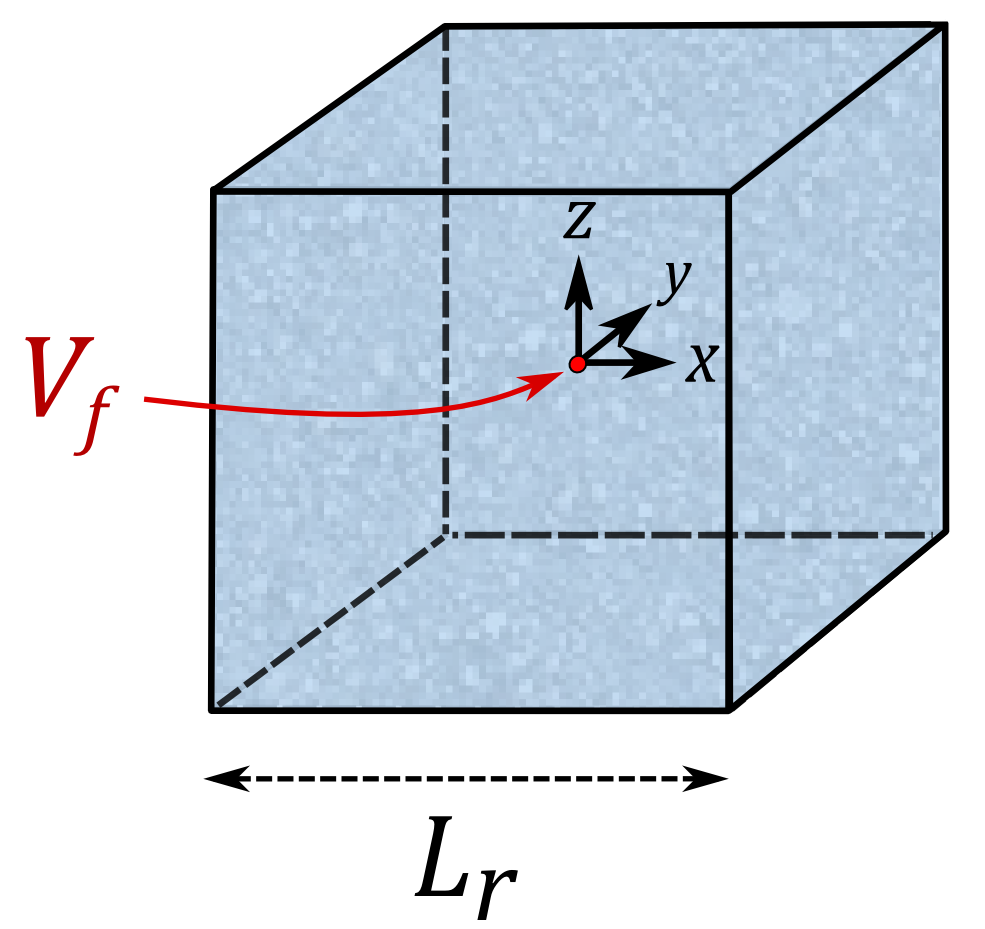
\includegraphics[width=0.45\textwidth]{./figs/immdot.png}
\caption{Схематичный вид задачи о мгновенном точечном источнике.}\label{fig:immdot}
\end{figure}
% 
%
%%
\begin{table}[h!]
\centering
%
\renewcommand{\arraystretch}{1.5}
\renewcommand{\tabcolsep}{6 pt} 
\begin{tabular}{|c|c|c|c|c|c|c|}
\hline
$L_r$ & $V_f$ & $t_{\text{start}}$ & $t_{\text{end}}$ & $\Delta t$\\
\hline
 $400.0$ м & $1.0 \text{ м}^3$ & $150.0$ с & $200.0$ с & $1.0$ с\\
\hline
\end{tabular}
%
\caption{Параметры для численного расчета задачи о мгновенном точечном источнике.}\label{tab:immdot}
\end{table}
%%
%
 

В расчетах использовалась тетраэдральная сетка, состоящая из 
$N_{nodes} = 68921$ узлов и $N_{elems} = 256000$ прямоугольных тетраэдров со сторонами $h_x = h_y = h_z = 1.0$ м.

В качестве величин для сравнения используются нормированные значения $\overline{p}$, $\overline{u}_r$:
%
\begin{equation*}
%
\overline{p} = \cfrac{p}{p_0}, \quad \overline{u}_r = \cfrac{u_r}{L_r},
%
\end{equation*}
%
где 
\begin{equation}
\label{eq:p0p0}
p_0 = \mu V_f / 2 k.
\end{equation}

Результаты расчетов и точное решение приведены на
рис.~\ref{fig::press_point_mom},
% и \ref{fig::disp_point_mom},
где показаны нормированные давления и перемещения в последовательные моменты времени
$t = 150, \; 165, \; 185, \; 200$ с. Как видно из рисунков, получено
хорошее совпадение с аналитическими результатами на все указанные моменты времени.

\begin{figure}[t!]
\centering
  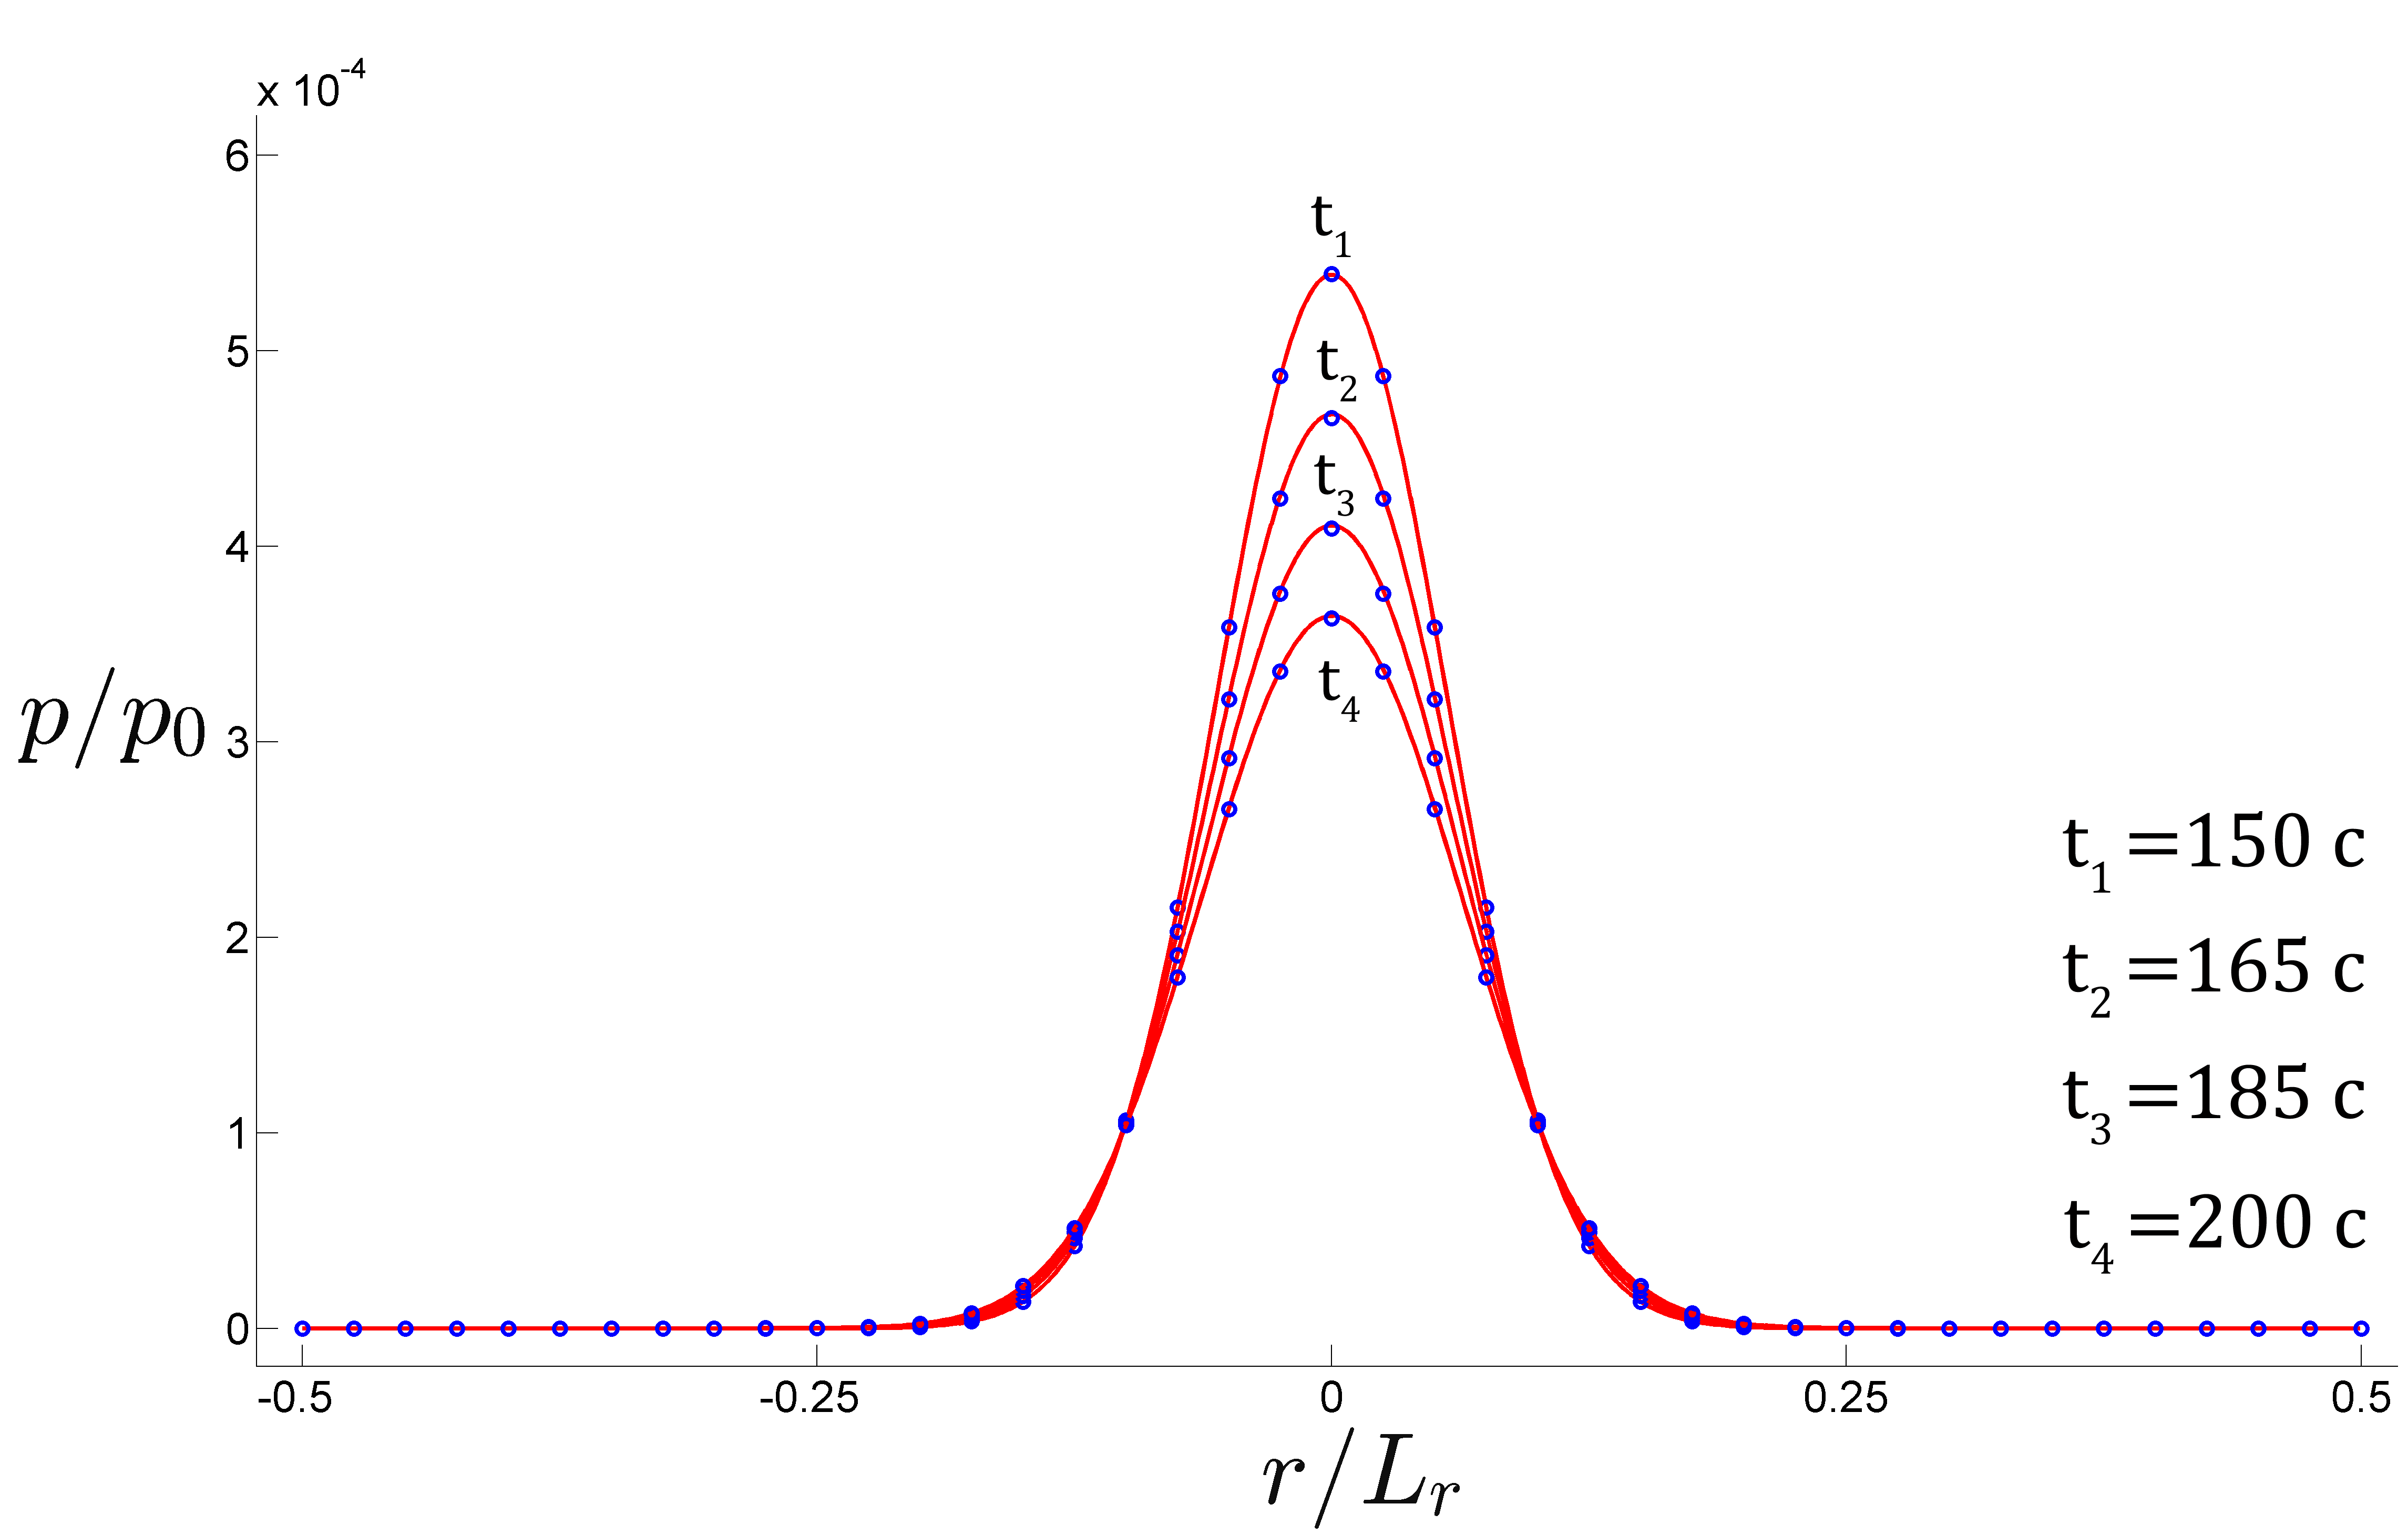
\includegraphics[width=0.8\textwidth]{figs/press_point_mom2.png}\\
  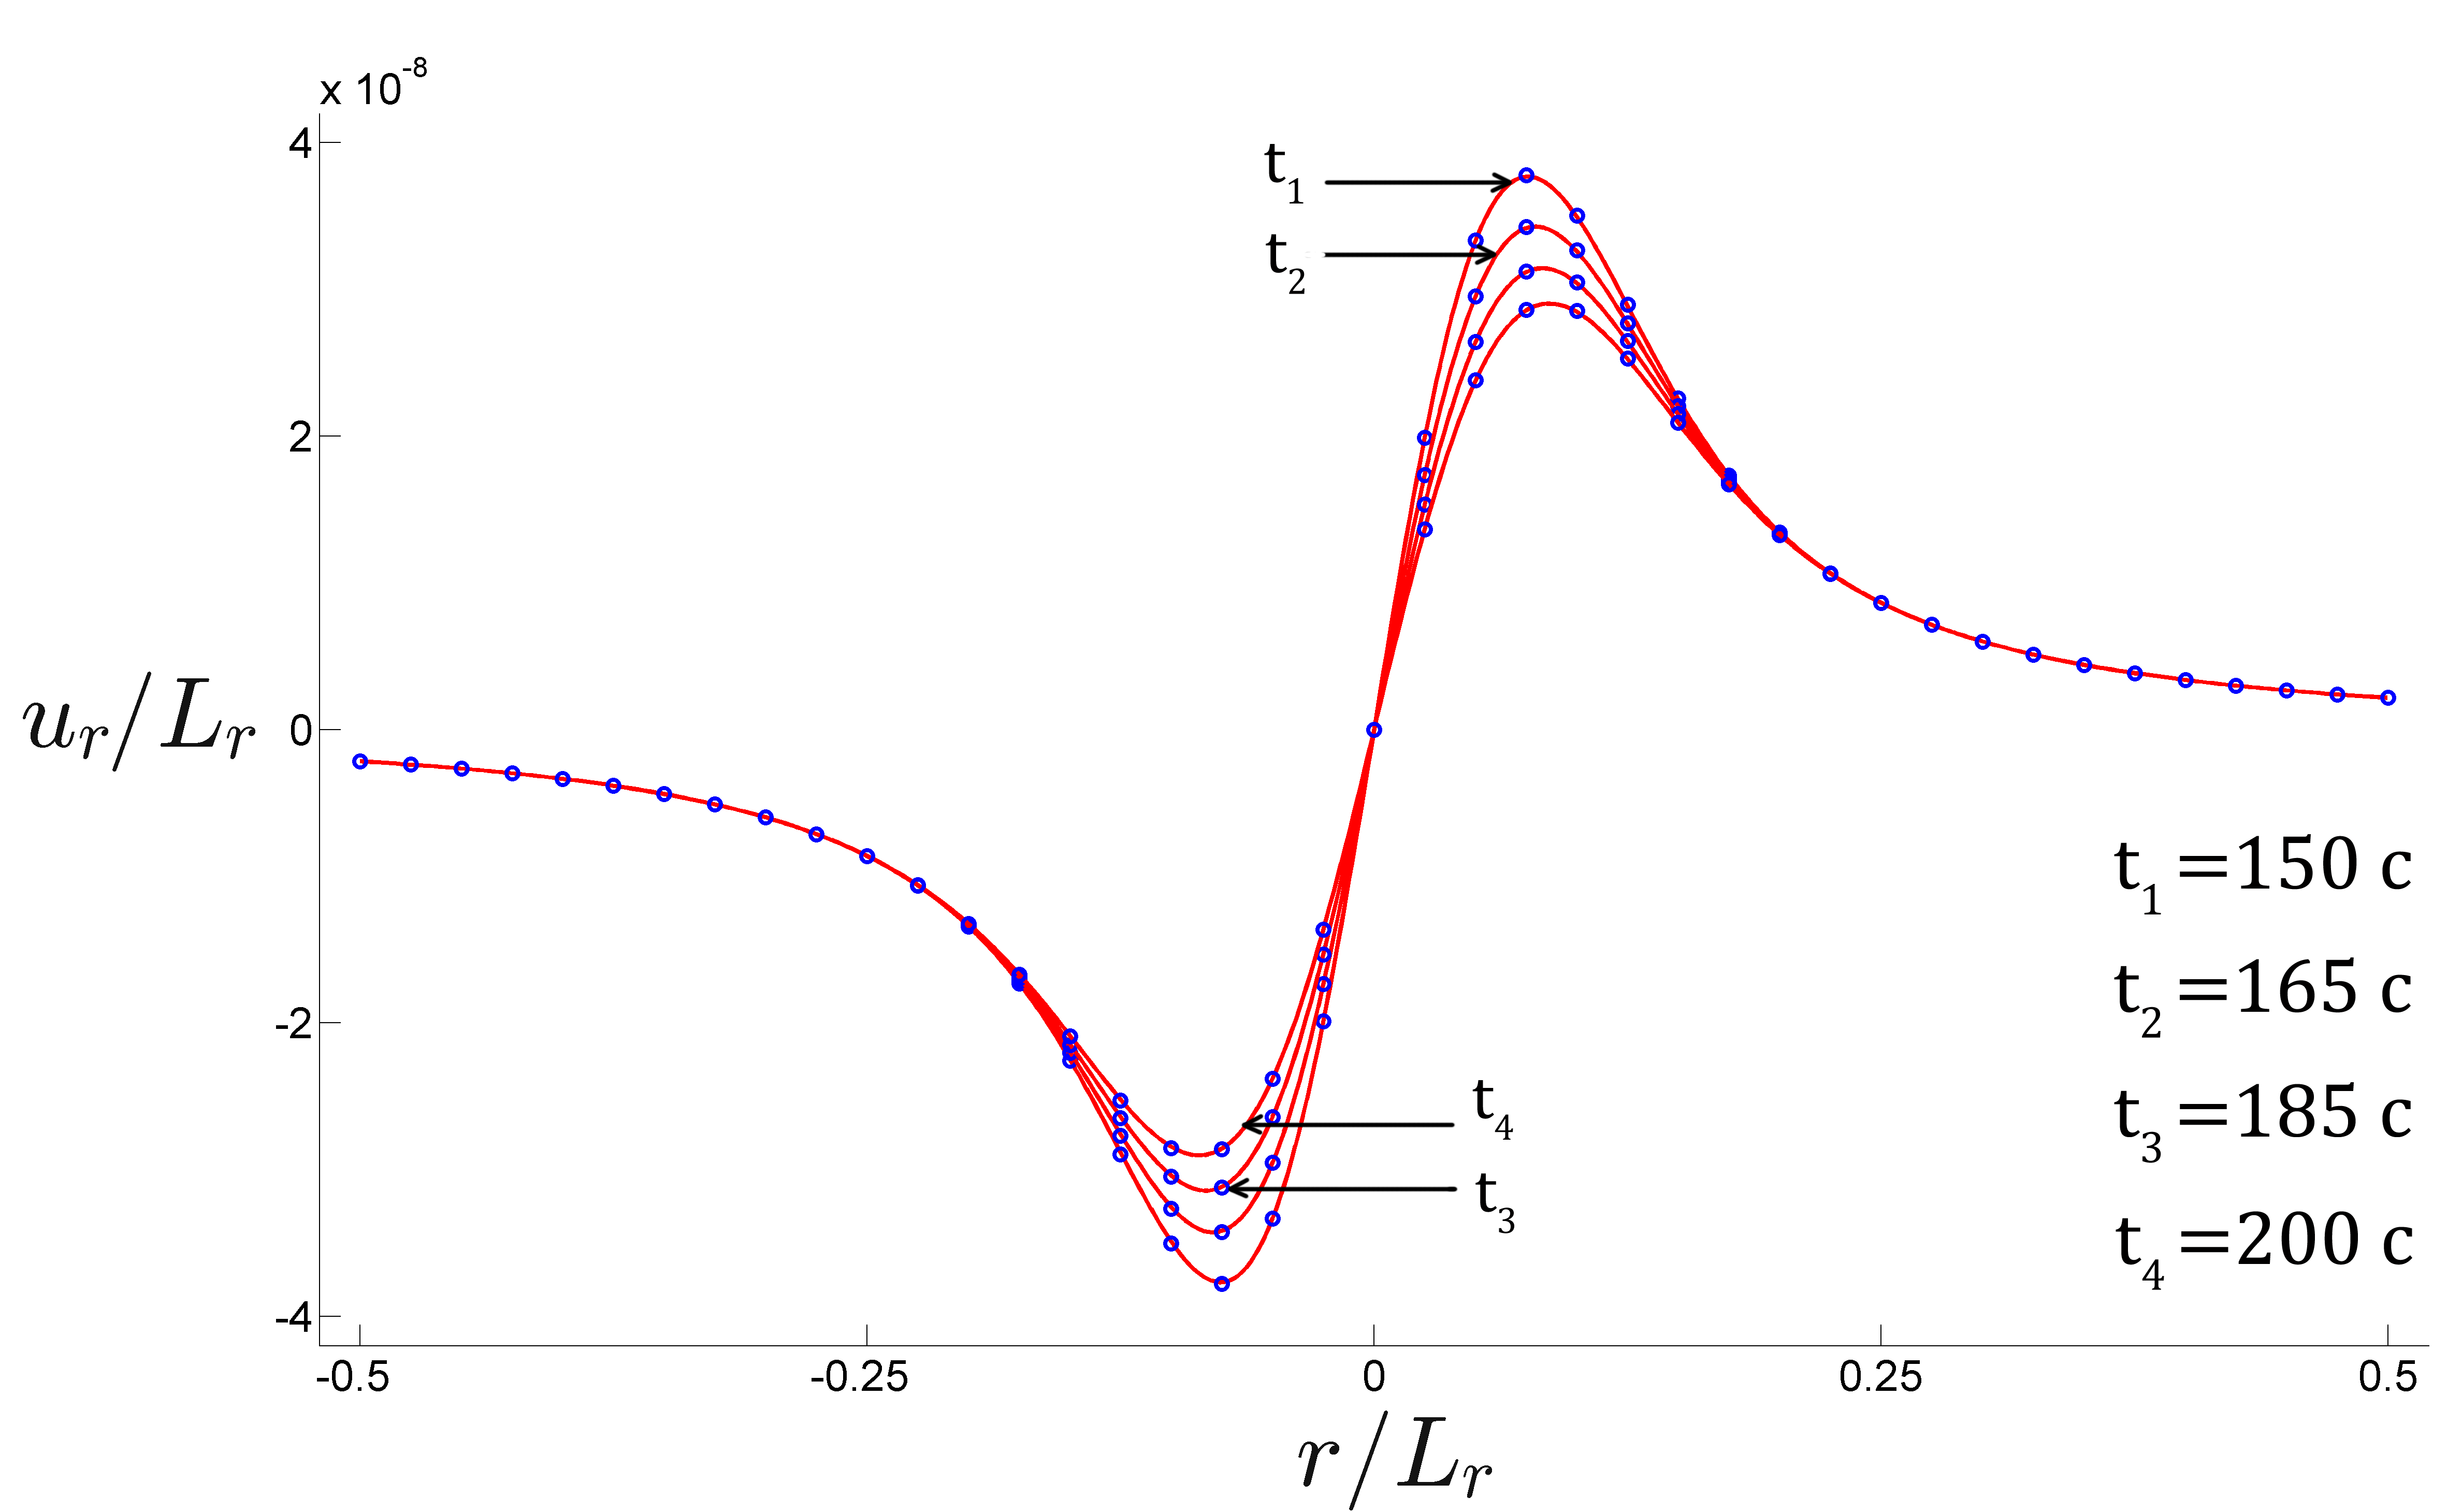
\includegraphics[width=0.8\textwidth]{figs/disp_point_mom2.png}
  \caption{ Задача о мгновенном точечном источнике. Нормированное давление (вверху) и перемещение (внизу) в различные моменты времени: красным
    цветом показано аналитическое решение, синим~--– результаты расчета.}
  \label{fig::press_point_mom}
\end{figure}
%
% \begin{figure}[t!]
% \centering
%   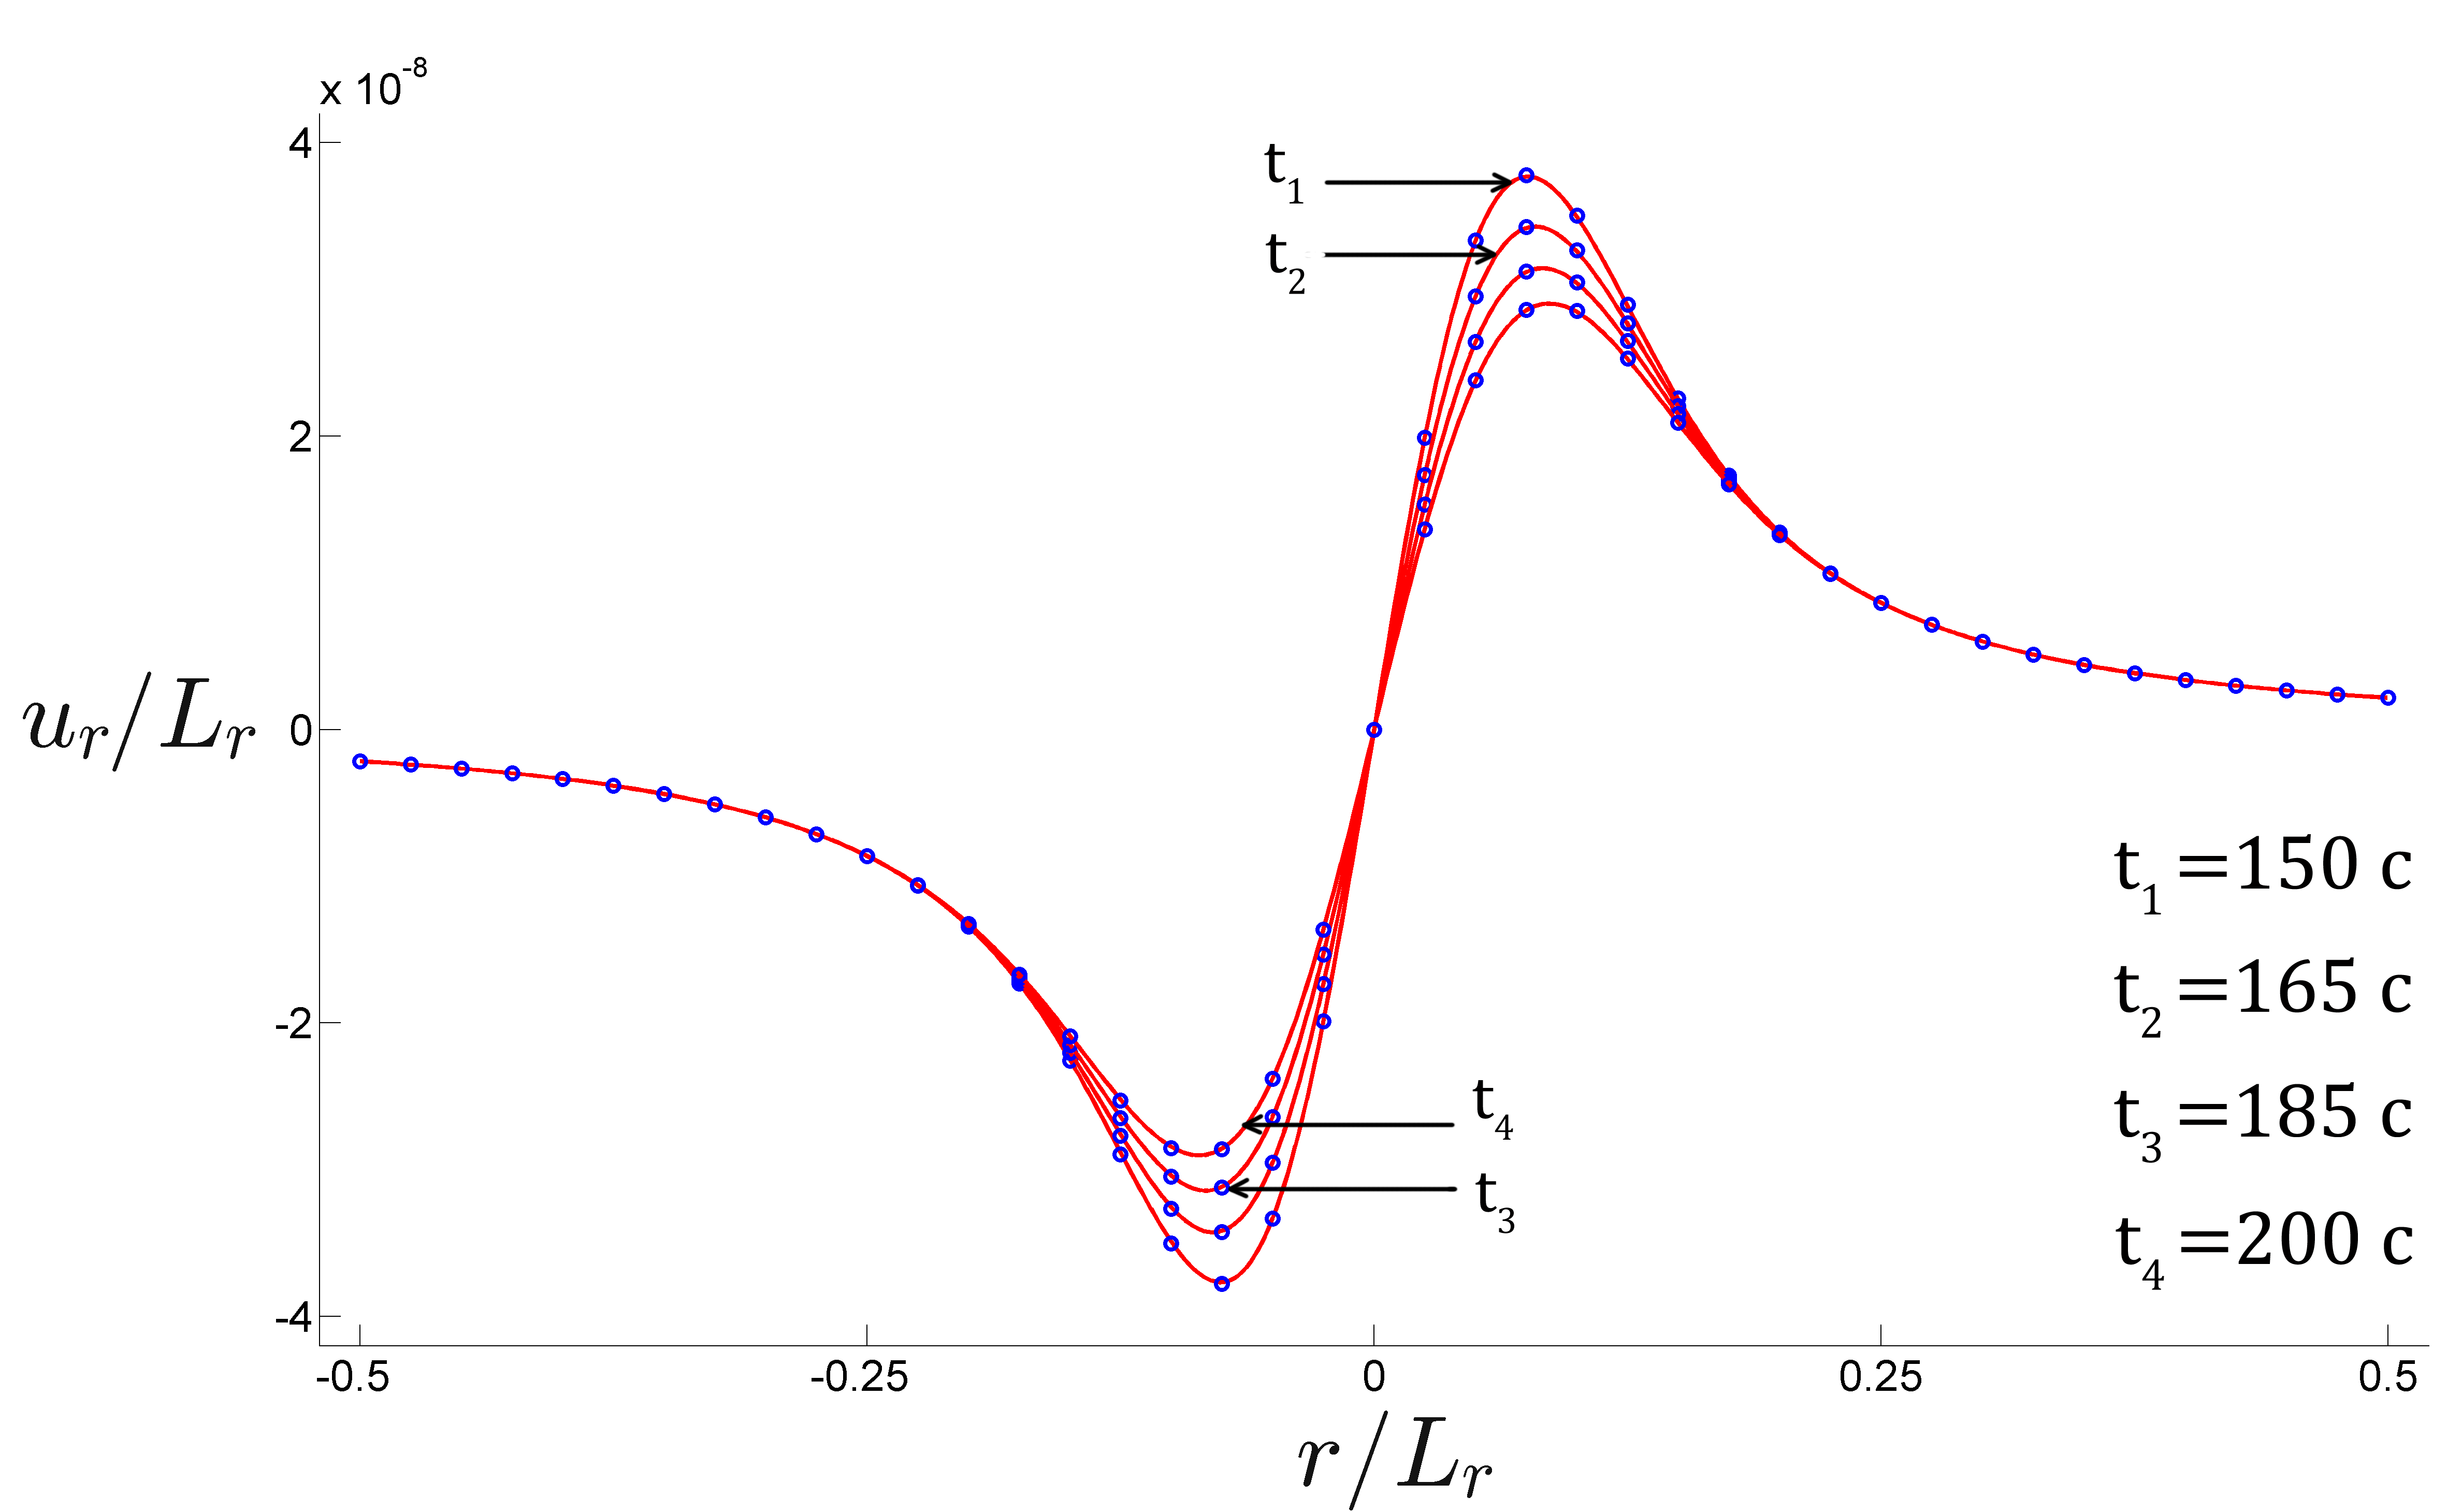
\includegraphics[width=0.8\textwidth]{figs/disp_point_mom2.png}
%   \caption{ Нормированное перемещение в различные моменты времени: красным
%   цветом показано аналитическое решение, синим – результаты расчета}
%   \label{fig::disp_point_mom}
% \end{figure}


%\newpage

\subsection{Задача о мгновенном линейном источнике}
Задача о линейном источнике является простейшей моделью, описывающей скважину в пороупругой среде.
Поэтому расчет этого теста является обязательной валидационной задачей для программных комплексов,
моделирующих течения в пороупругих средах.

Задача ставится следующим образом: в бесконечной невозмущенной
пороупругой среде в момент времени $t=0$ с на некоторой линии
происходит впрыскивание массы флюида с линейной плотностью $M_f$
объемом $V_f = M_f/\rho^0_f$, что мгновенно приводит к деформации
попроупругой среды.  В такой постановке решение задачи, очевидно,
обладает радиальной симметрией.
 
Аналитическое решение задачи записывается следующим образом~\cite{coussy_2004}:
\begin{equation}
\label{eq:immlinep}
%
p(r,t) = \frac{V_f}{4\pi (k/\mu) t} \exp{\left( -\frac{r^2}{4 c_f t}\right)}, \\
%
\end{equation}
%
\begin{equation}
\label{eq:immlinur}
u_r(r,t) = \frac{3bM}{3K_u+4\nu} \cdot \frac{V_f}{2 \pi r} \left[1 - \exp{\left( -\frac{r^2}{4 c_f t}\right)} \right],
\end{equation}
%
%\igma_{rr} = \frac{bM\mu}{K_u+\frac{4}{3}\mu} \frac{V_f}{2\pi r^2} \left[1 - \exp{\left( -\frac{r^2}{4 c_f t}\right)} \right] \\
%
%\sigma_{\theta\theta} = \frac{bM\mu}{K_u+\frac{4}{3}\mu} \frac{V_f}{2\pi r^2} \left[1 - \left(1+\frac{r^2}{2c_f t}\right) \exp{\left( -\frac{r^2}{4 c_f t}\right)} \right] \\
%
%\sigma_{zz} = \frac{bM\mu}{K_u+\frac{4}{3}\mu} \frac{V_f}{2\pi c_f t} \left[1 - \exp{\left( -\frac{r^2}{4 c_f t}\right)} \right]
%\end{eqnarray}
где $c_f$ определяется согласно формуле~\eqref{eq:cf}.

Для расчетов использовалась область с линейными размерами $L_x$, $L_y$, $L_z$,
в центре которой располагался линейный источник,
проходящий через точки с координатами $(0, 0, 0)$ и $(0, 0, L_z)$.
Схематично постановка задачи представлена на рис.~\ref{fig:immline}.
Конкретные значения используемых для расчетов параметров приведены в табл.~\ref{tab:immline}.

На границе расчетной области перемещение задавались согласно 
точному решению~\eqref{eq:immlinep}, для давления на всех границах использовалось условие
нулевого потока $\partial p/ \partial n = 0$. Начальное распределение задавалось
согласно аналитическому решению на момент времени $t_{\text{start}}$.
%
\begin{figure}[t!]
\centering
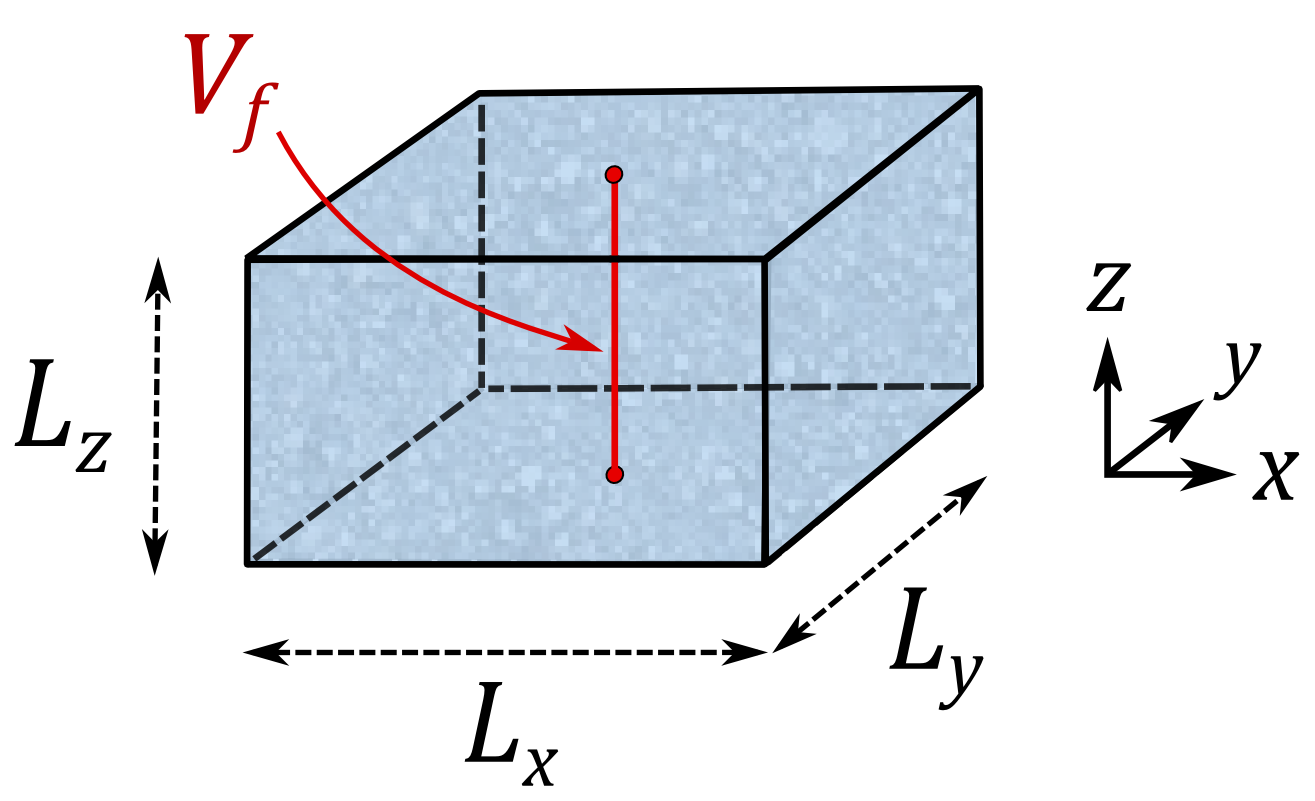
\includegraphics[width=0.65\textwidth]{./figs/immline.png}
\caption{Схематичный вид задачи о мгновенном линейном источнике.}\label{fig:immline}
\end{figure}
% 
%
%%
\begin{table}[h!]
\centering
%
\renewcommand{\arraystretch}{1.5}
\renewcommand{\tabcolsep}{6 pt} 
\begin{tabular}{|c|c|c|c|c|c|c|}
\hline
$L_x$ & $L_y$ & $L_z$ & $V_f$ & $t_{\text{start}}$ & $t_{\text{end}}$ & $\Delta t$\\
\hline
 $400.0$ м & $400.0$ м & $10.0$ м & $1.0 \text{ м}^3$ & $150.0$ с & $200.0$ с & $1.0$ с\\
\hline
\end{tabular}
%
\caption{Параметры для численного расчета задачи о мгновенном линейном источнике.}\label{tab:immline}
\end{table}
%%
%

В расчетах использовалась тетраэдральная сетка, состоящая из 
$N_{nodes} = 5043$ узлов и $N_{elems} = 12800$ прямоугольных тетраэдров со сторонами $h_x = h_y = h_z = 1.0$ м.

В качестве величин для сравнения используются нормированные значения $\overline{p}$, $\overline{u}_r$:
%
\begin{equation*}
%
\overline{p} = \cfrac{p}{p_0}, \quad \overline{u}_r = \cfrac{u_r}{L_r},
%
\end{equation*}
%
где $p_0$ определялось согласно формуле~\eqref{eq:p0p0}, $L_r = L_x = L_y$.
 

Результаты расчетов и точное решение приведены на
рис.~\ref{fig::press_line_mom}
% и \ref{fig::disp_line_mom},
где показаны нормированные давления и перемещения в последовательные моменты времени
$t = 150, \; 165, \; 185, \; 200$ с. Как видно из рисунков, получено
хорошее совпадение с аналитическими результатами на все указанные моменты времени.

\begin{figure}[t!]
\centering
  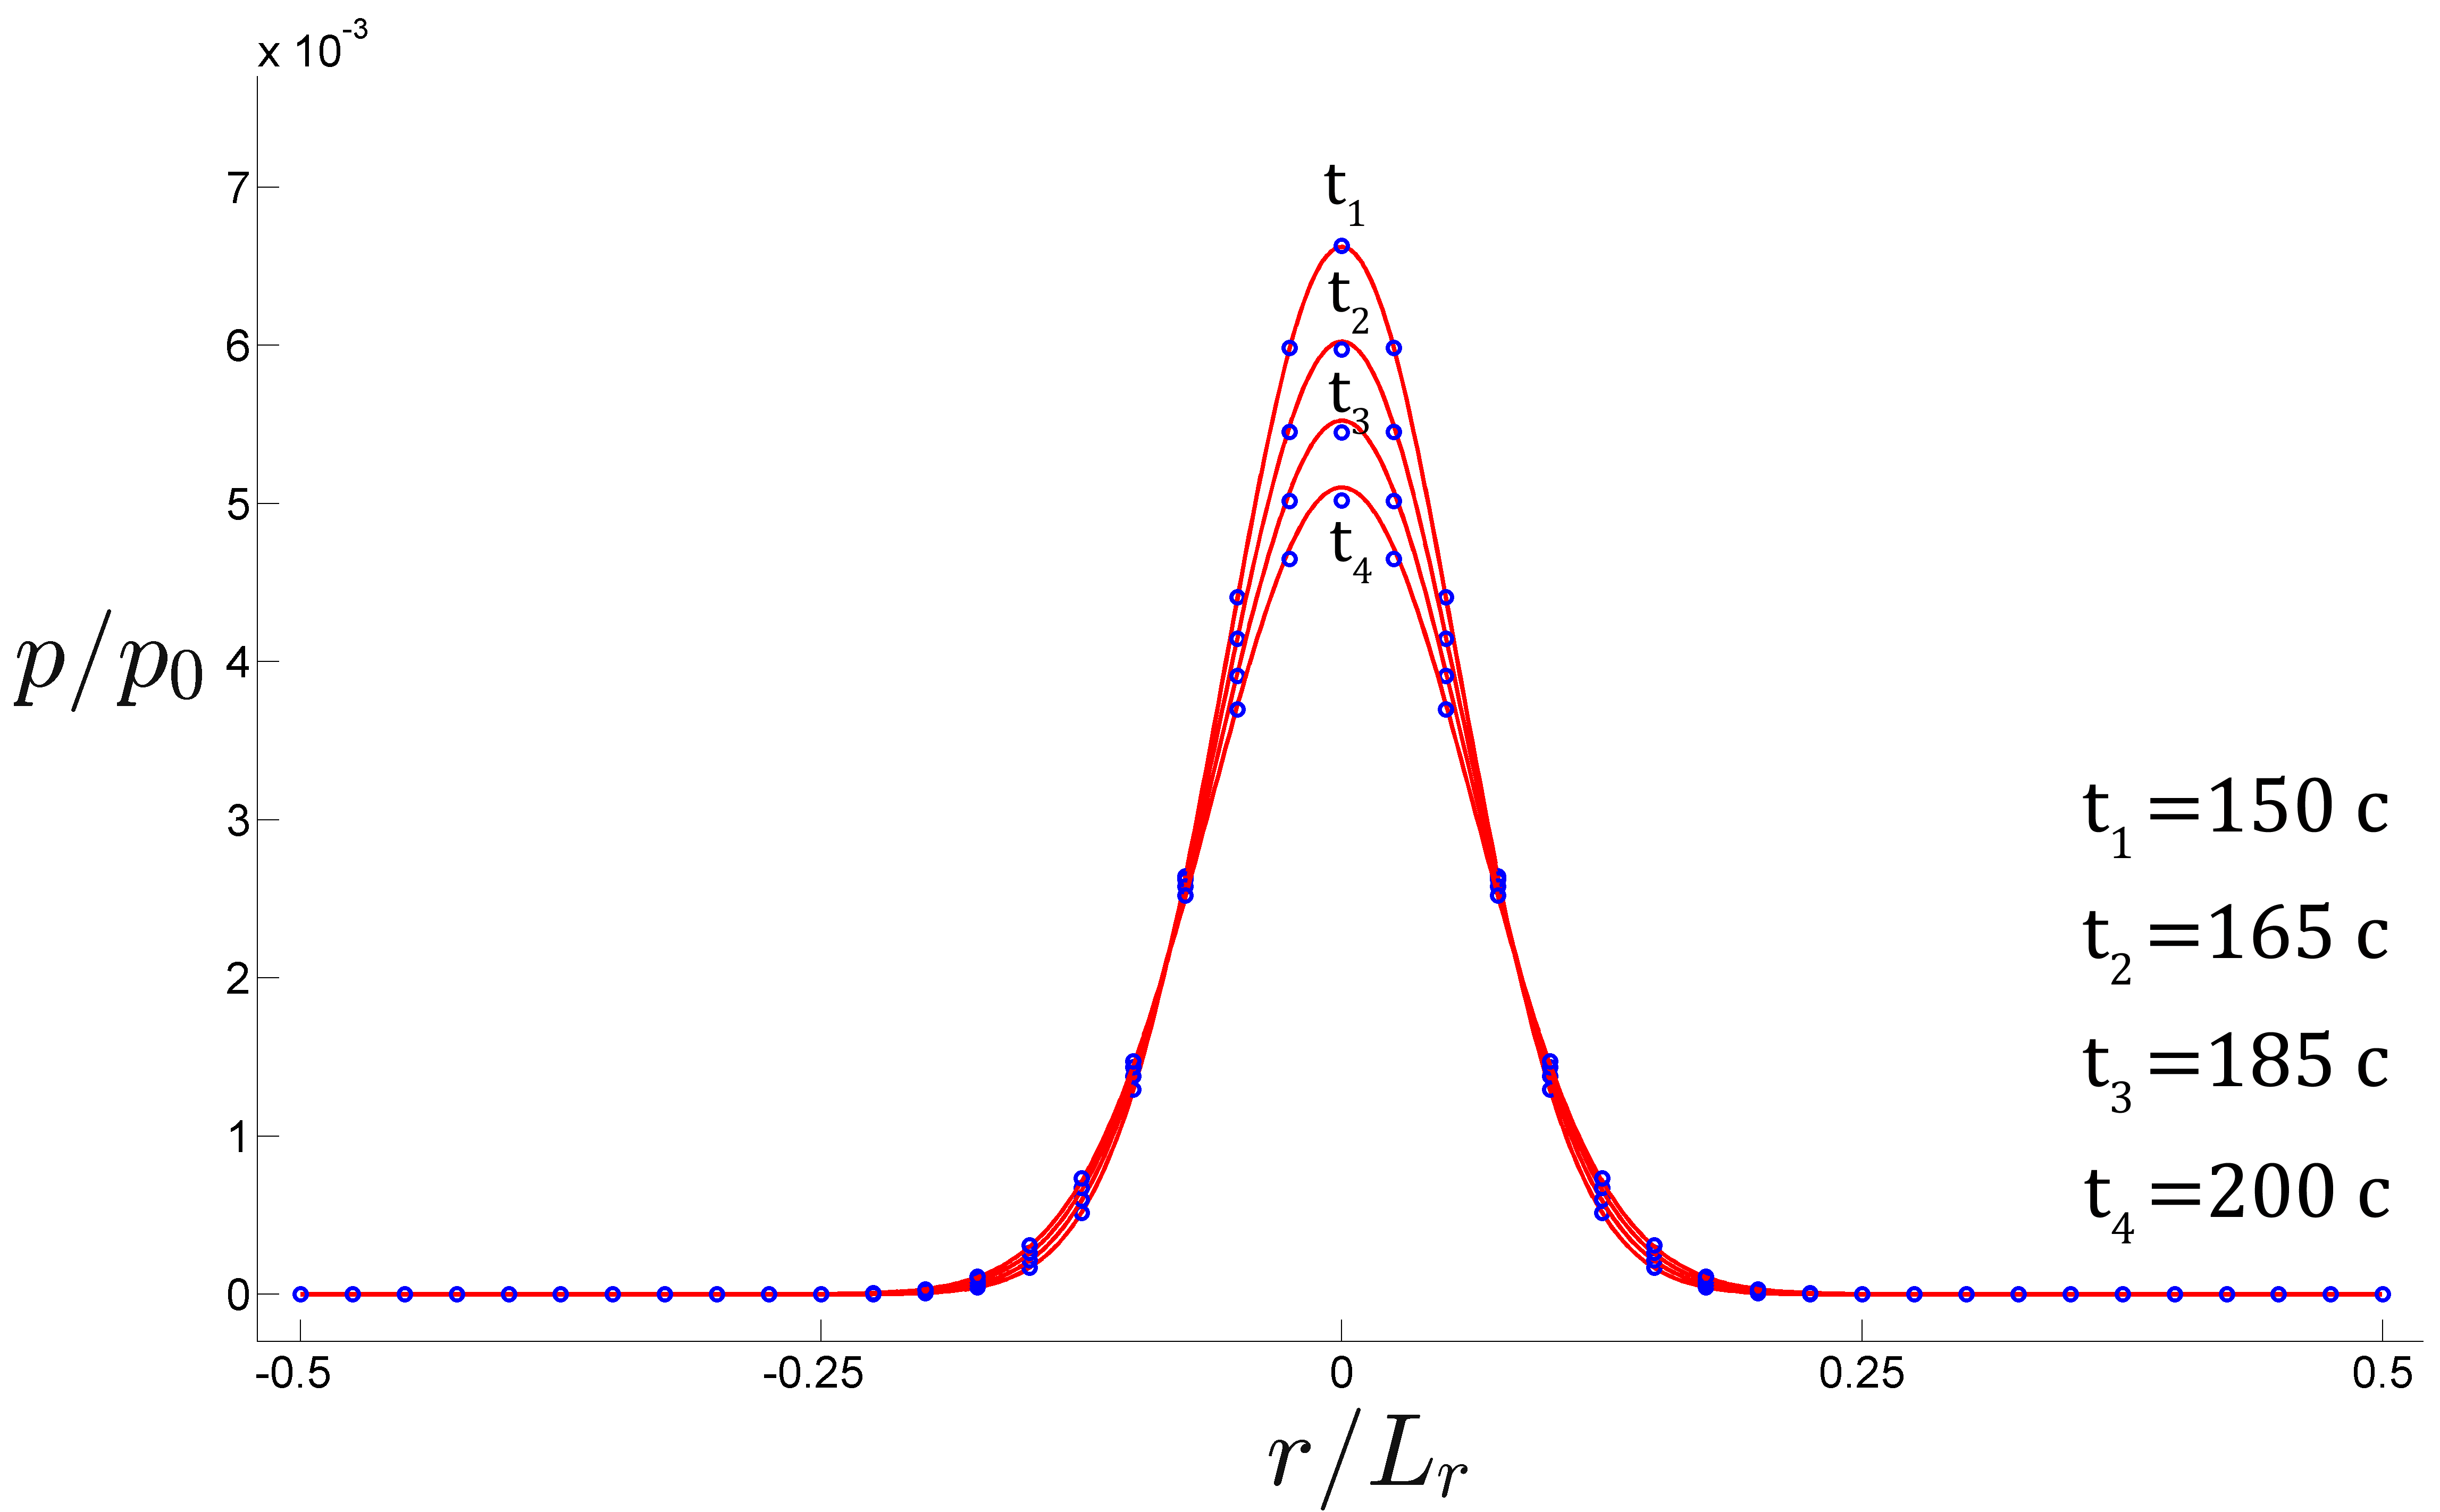
\includegraphics[width=0.8\textwidth]{figs/press_line_mom2.png}\\
  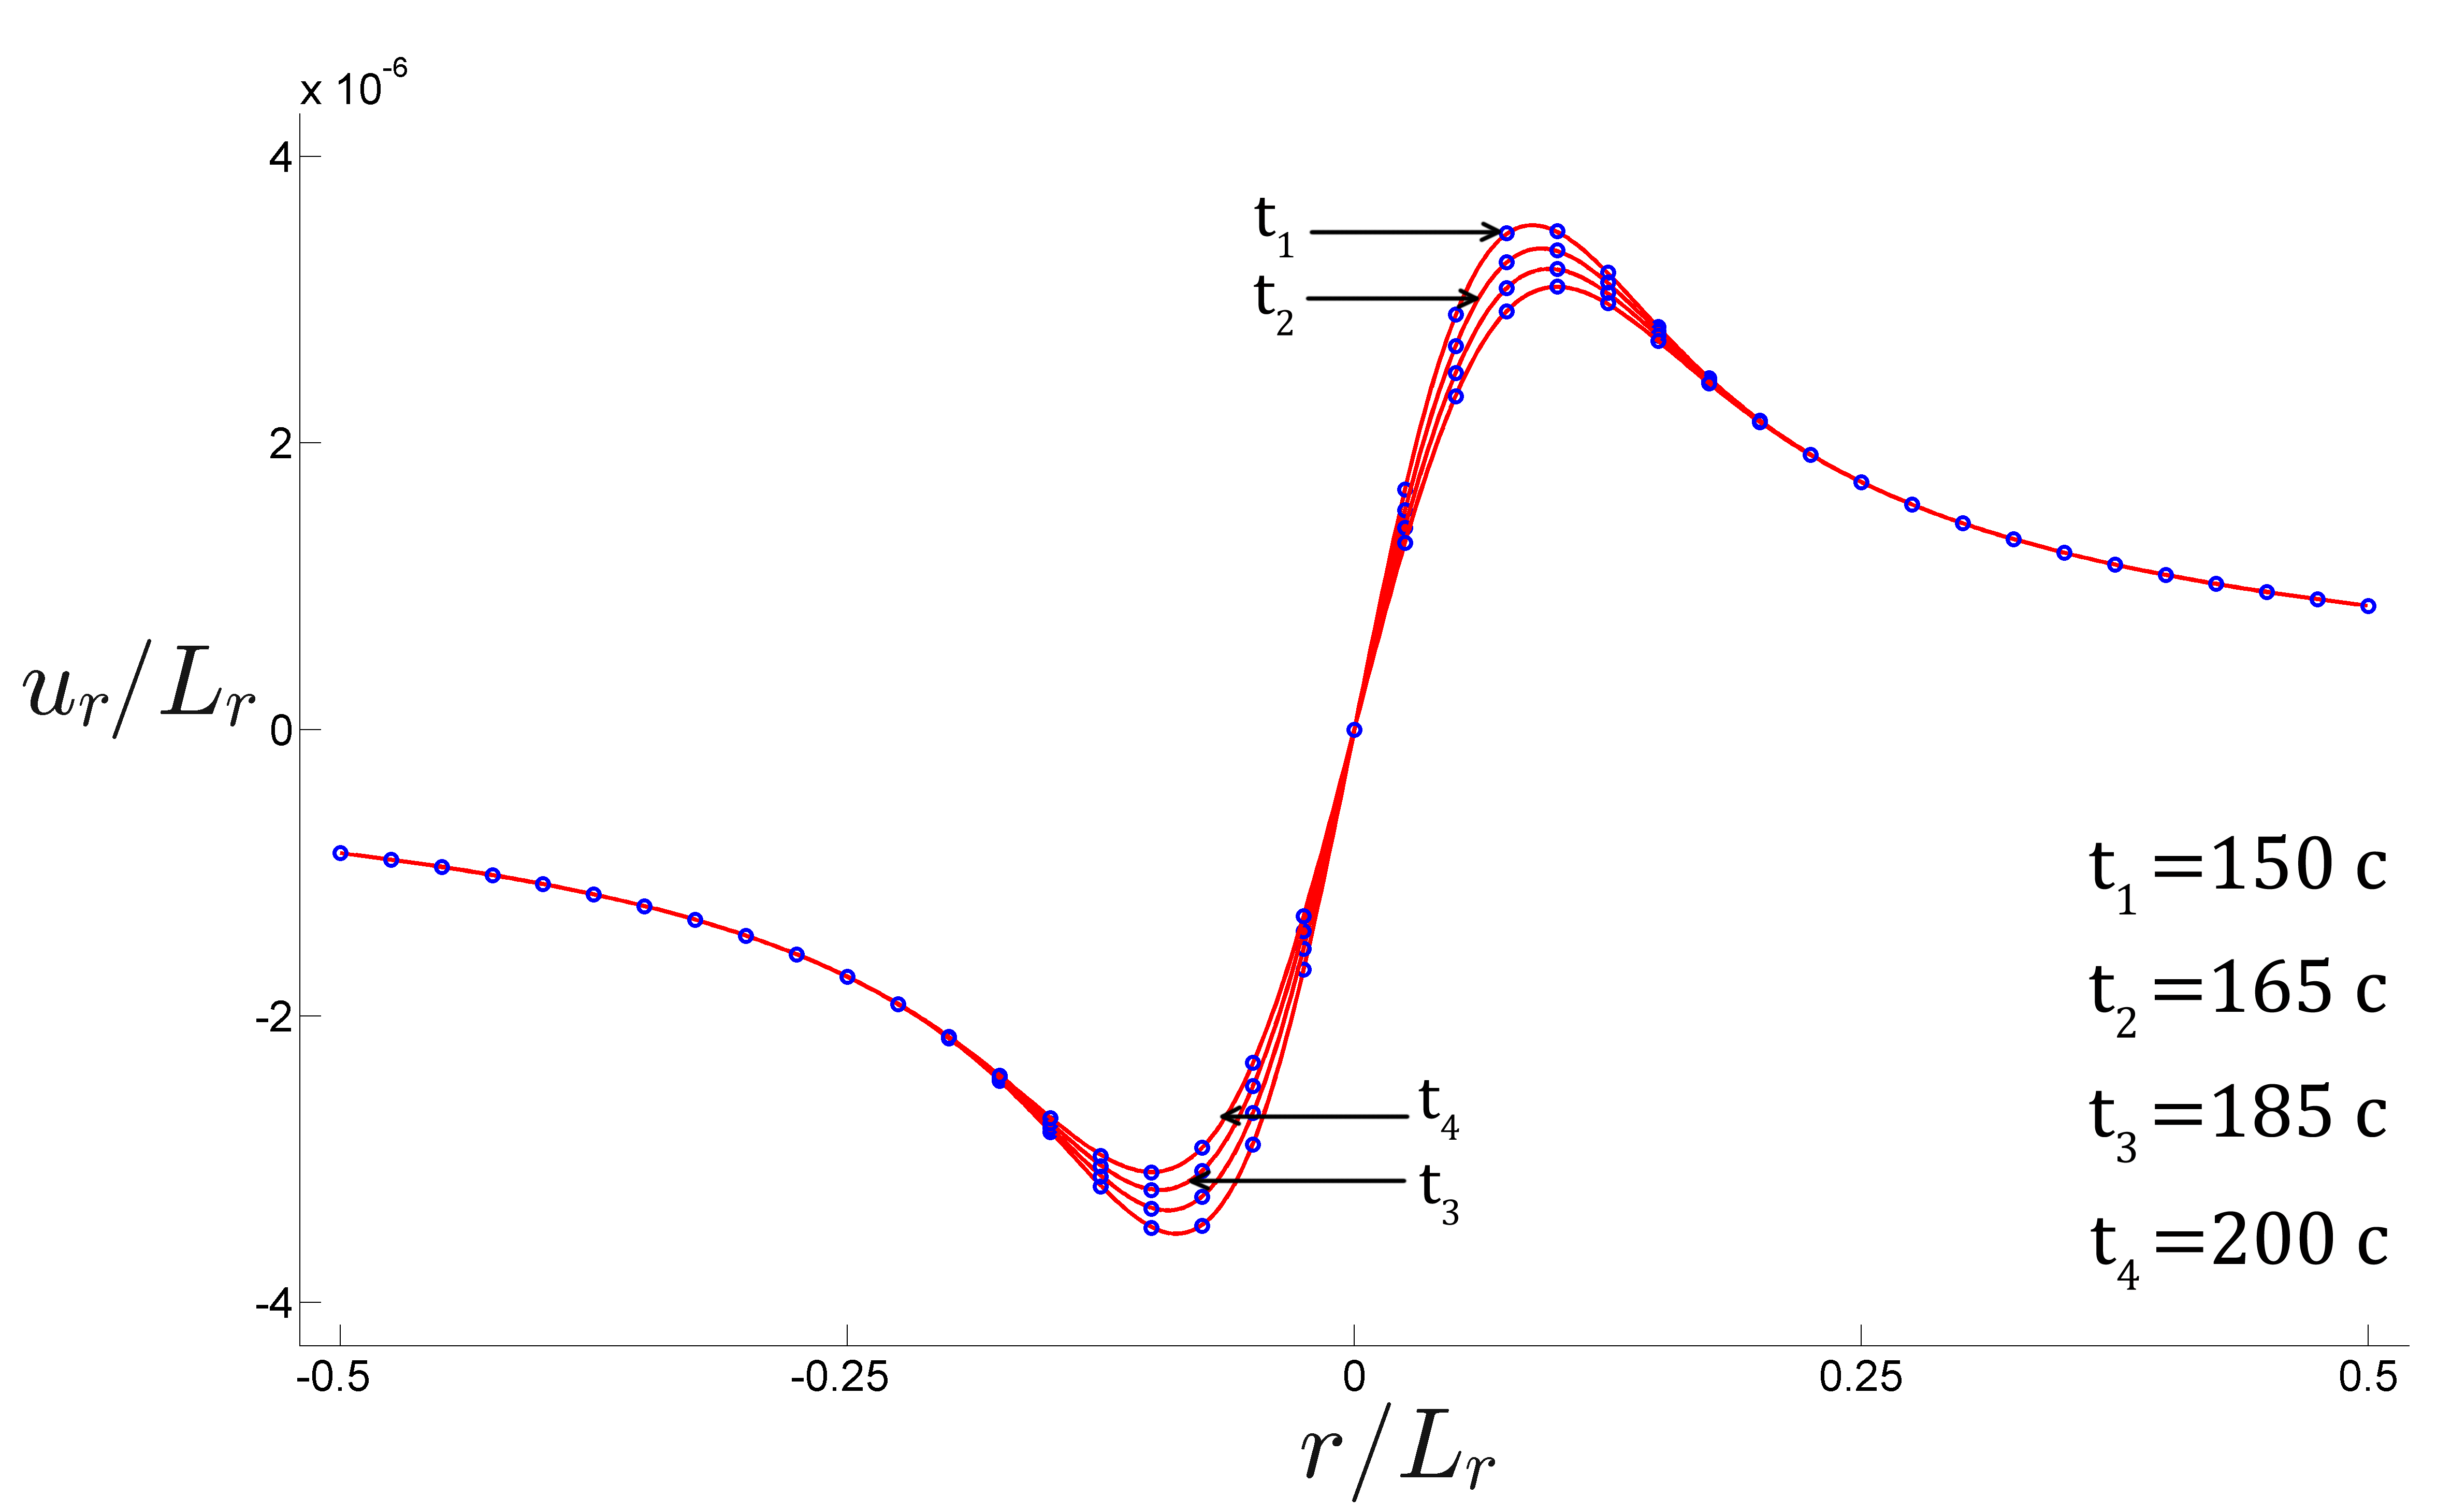
\includegraphics[width=0.8\textwidth]{figs/disp_line_mom2.png}
  \caption{ Задача о мгновенном линейном источнике. Нормированное давление (вверху) и перемещение (внизу) в различные моменты времени: красным
цветом показано аналитическое решение, синим~--– результаты расчета.}
  \label{fig::press_line_mom}
\end{figure}
% %
% \begin{figure}[b!]
% \centering
%   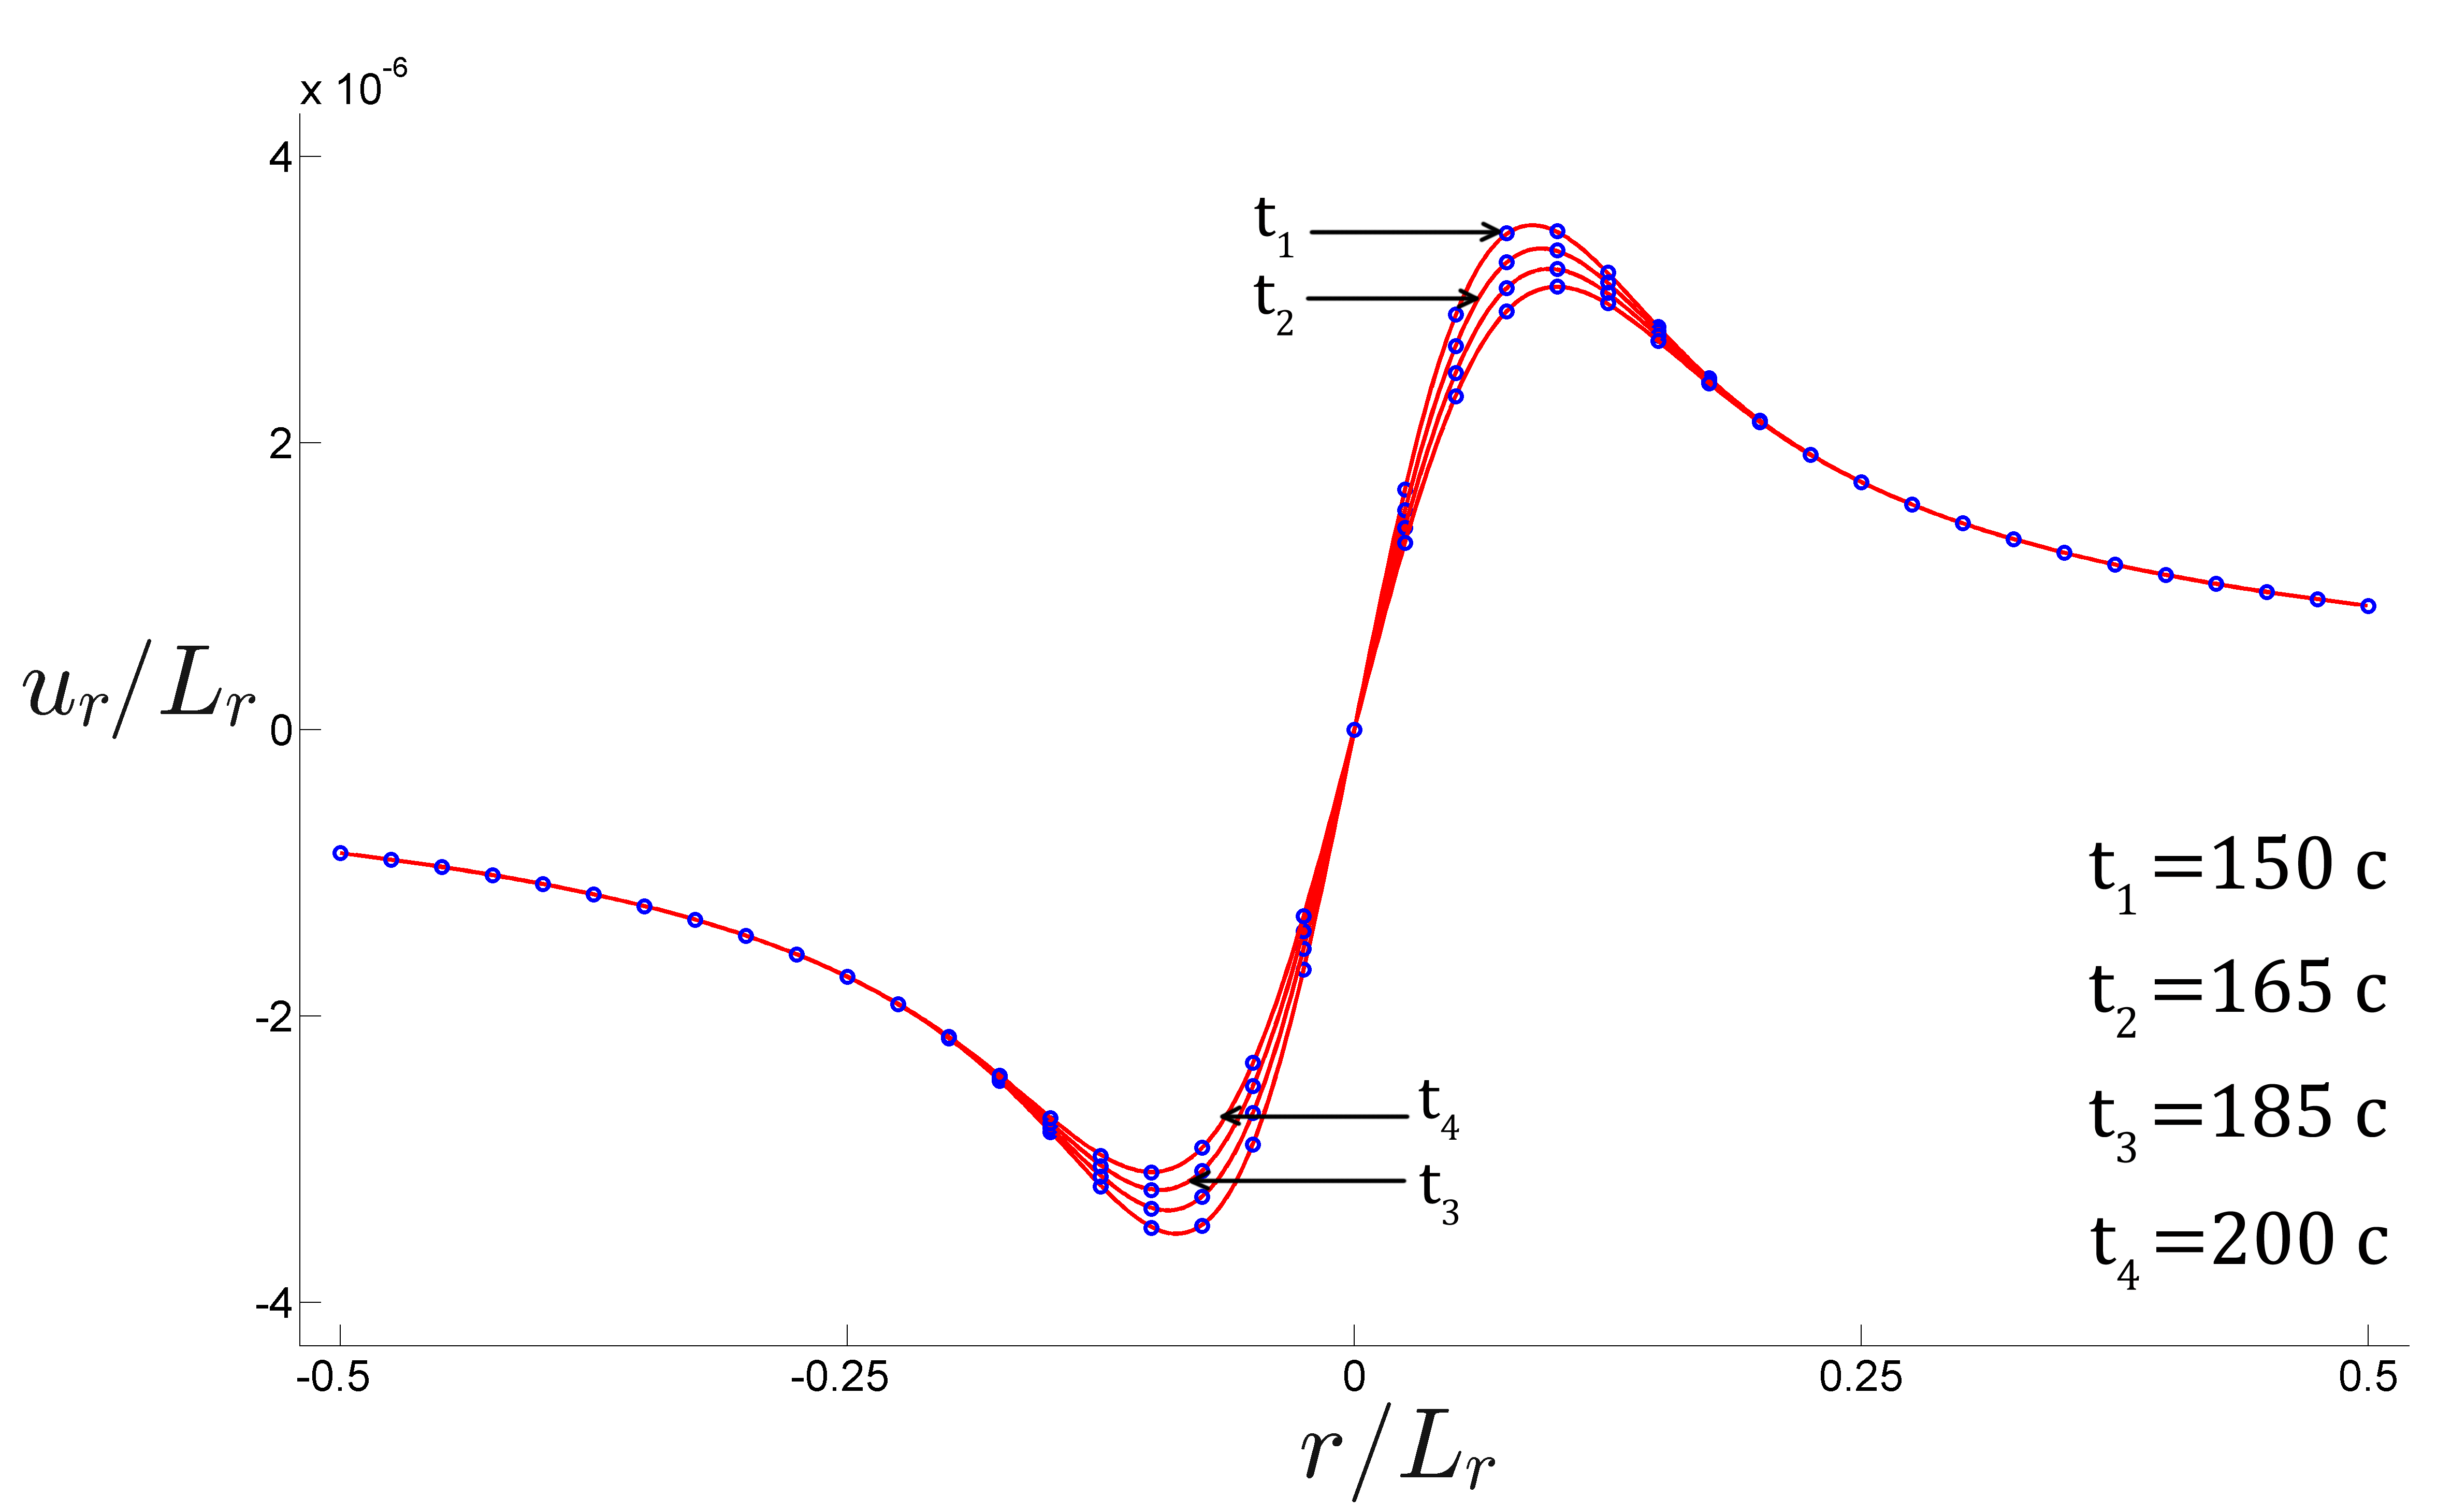
\includegraphics[width=0.88\textwidth]{figs/disp_line_mom2.png}
%   \caption{ Нормированное перемещение в различные моменты времени: красным
% цветом показано аналитическое решение, синим~--– результаты расчета }
%   \label{fig::disp_line_mom}
% \end{figure}

%\newpage

\subsection{Задача о постоянном линейном источнике}

На основе решения задачи о мгновенном линейном источнике в пороупругой среде
путем суперпозиции решений можно получить решение для линейного постоянного источника~\cite{wang_2000}:
%
\begin{equation}
\label{eq:constlinep}
p(r,t) = \frac{V_f}{4\pi (k/\mu)} E_1 \left(\frac{r^2}{4 c_f t}\right),
\end{equation}
%
\begin{multline}
\label{eq:constlinur}
u_r(r,t) = \frac{3b}{(3K+4\nu)(k/\mu)} \cdot \frac{V_f}{8 \pi} r \\ 
\cdot
\left\{ \frac{4 c_f t}{r^2}\left[1 - \exp{\left( -\frac{r^2}{4 c_f t}\right)} \right] + E_1 \left(\frac{r^2}{4 c_f t}\right) \right\},
\end{multline}
%
где
%
\begin{equation*}
E_1(u) = \int\limits_u^\infty \frac{\exp(-\xi)}{\xi} d\xi.
\end{equation*}

В данных выражениях $V_f$ имеет смысл объема жидкости, притекающего через источник в единицу времени.

Область, граничные условия и расчетная сетка брались аналогично таковым для задачи
о мгновенном линейном источнике. Объем притока в единицу времени задавался как $V_f = 1 \text{м}^3 / \text{с}$.
Расчет начинался с момента времени $t_{\text{start}}=1000$ c, проводился с шагом $\Delta t = 100$ c до времени $t_{\text{end}}=1800$ c.



Результаты расчетов приведены на
рис.~\ref{fig::press_const_line_source},
% и~\ref{fig::disp_const_line_source},
где показано распределение нормированного давления и перемещения в начальный и конечный моменты времени.
Как видно из рисунков, получено приемлемое совпадение с аналитическими результатами. Различия связаны с невозможностью
разрешить сингулярность от источника с помощью используемых в программном комплексе методов.

\begin{figure}[t!]
\centering
  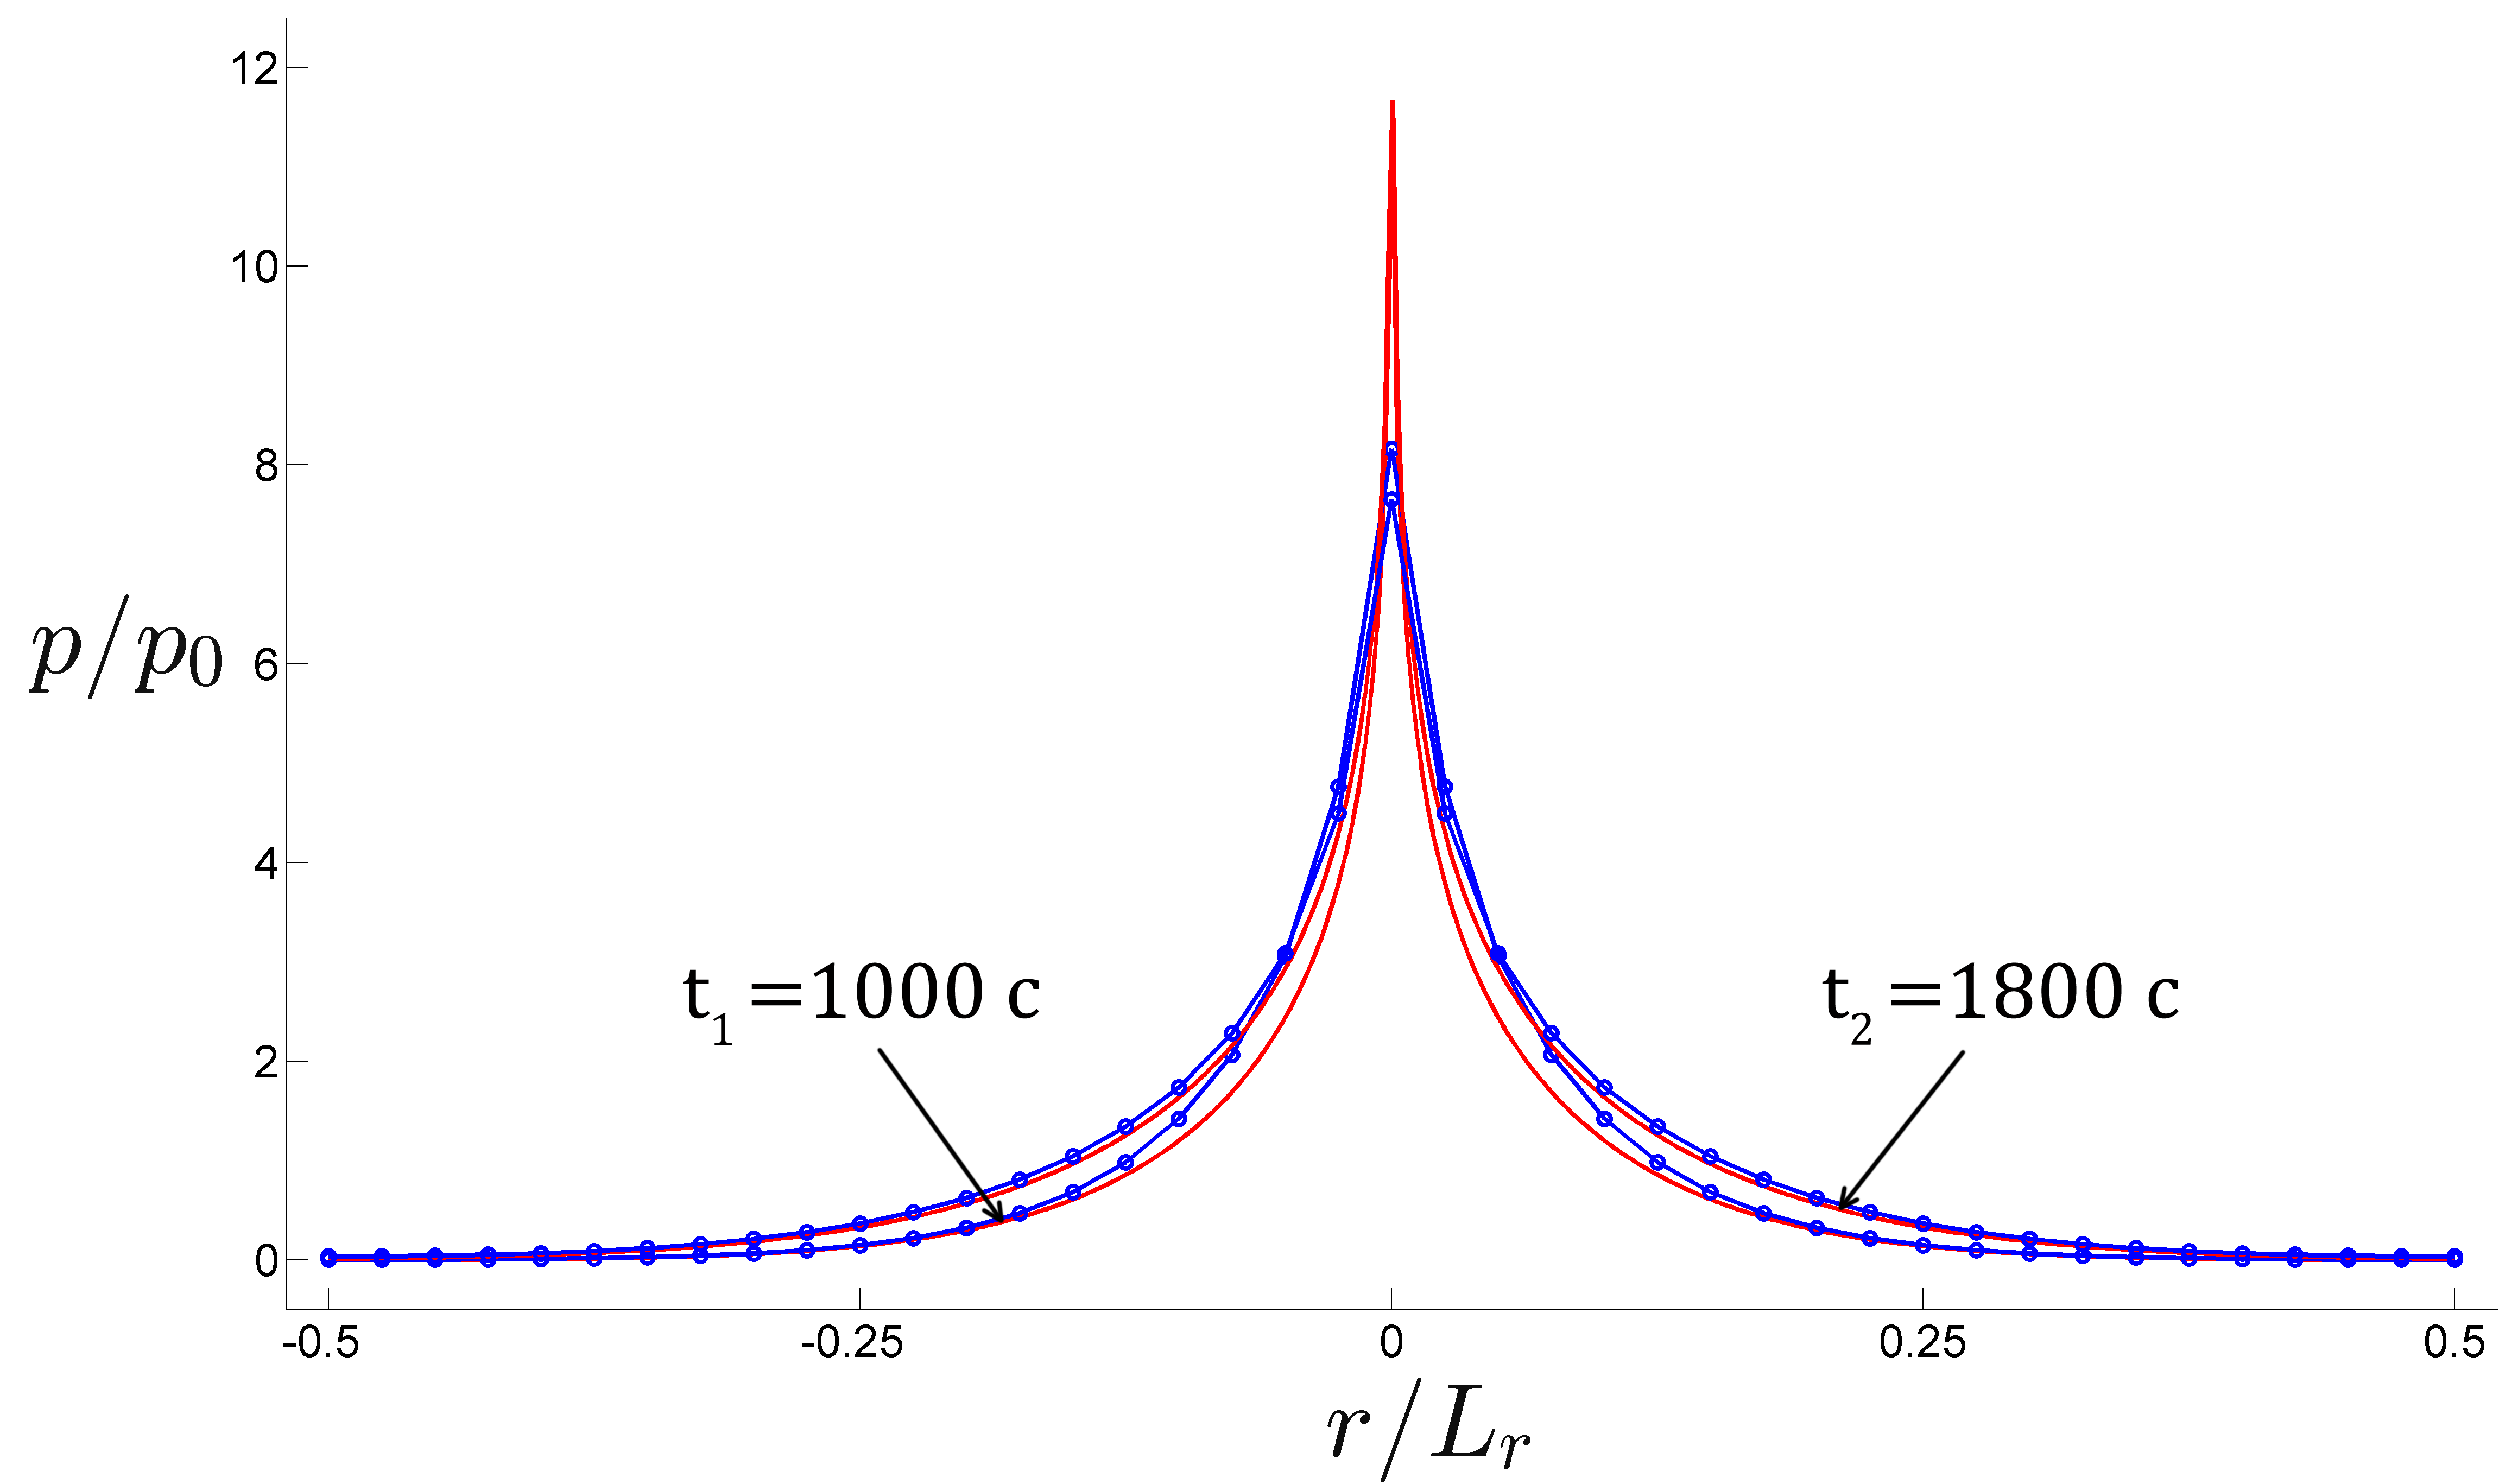
\includegraphics[width=0.8\textwidth]{figs/press_const_line_source2.png}\\
  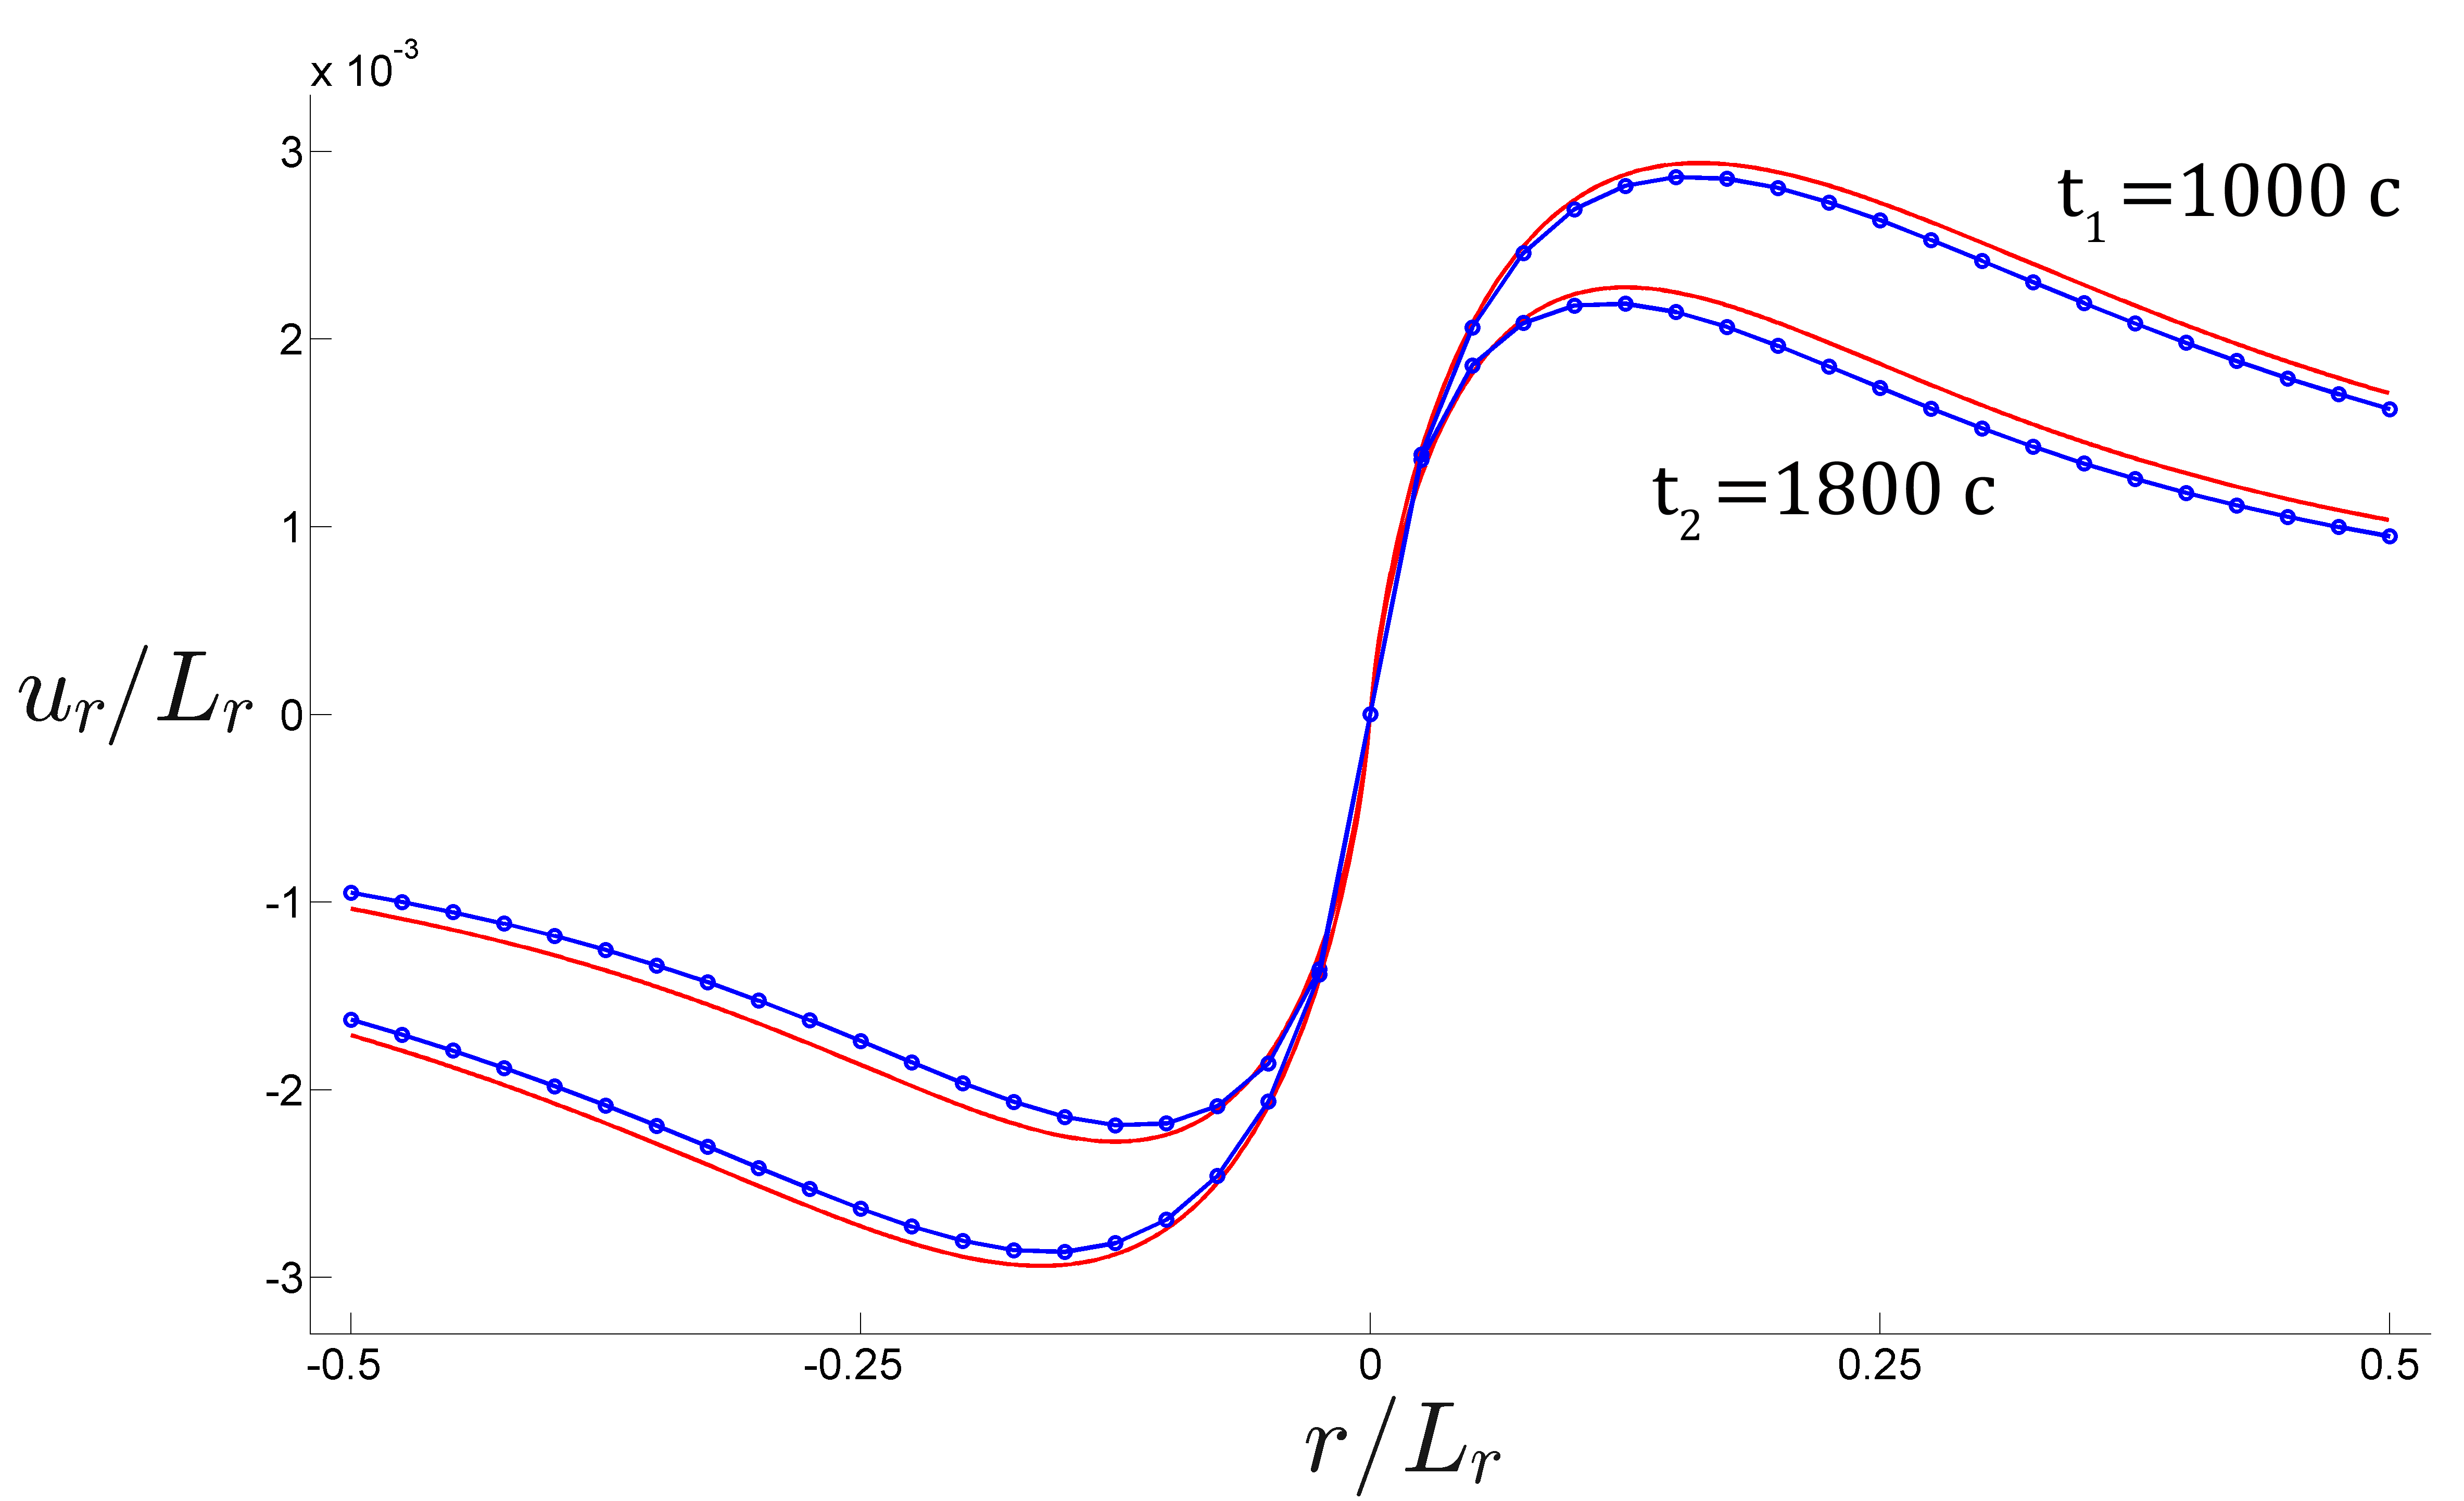
\includegraphics[width=0.8\textwidth]{figs/disp_const_line_source2.png}
  \caption{ Задача о постоянном линейном источнике. Нормированное давление (вверху) и перемещение (внизу) в различные моменты времени: красным
цветом показано аналитическое решение, синим~--– результаты расчета.}
  \label{fig::press_const_line_source}
\end{figure}

% \begin{figure}[h!]
% \centering
%   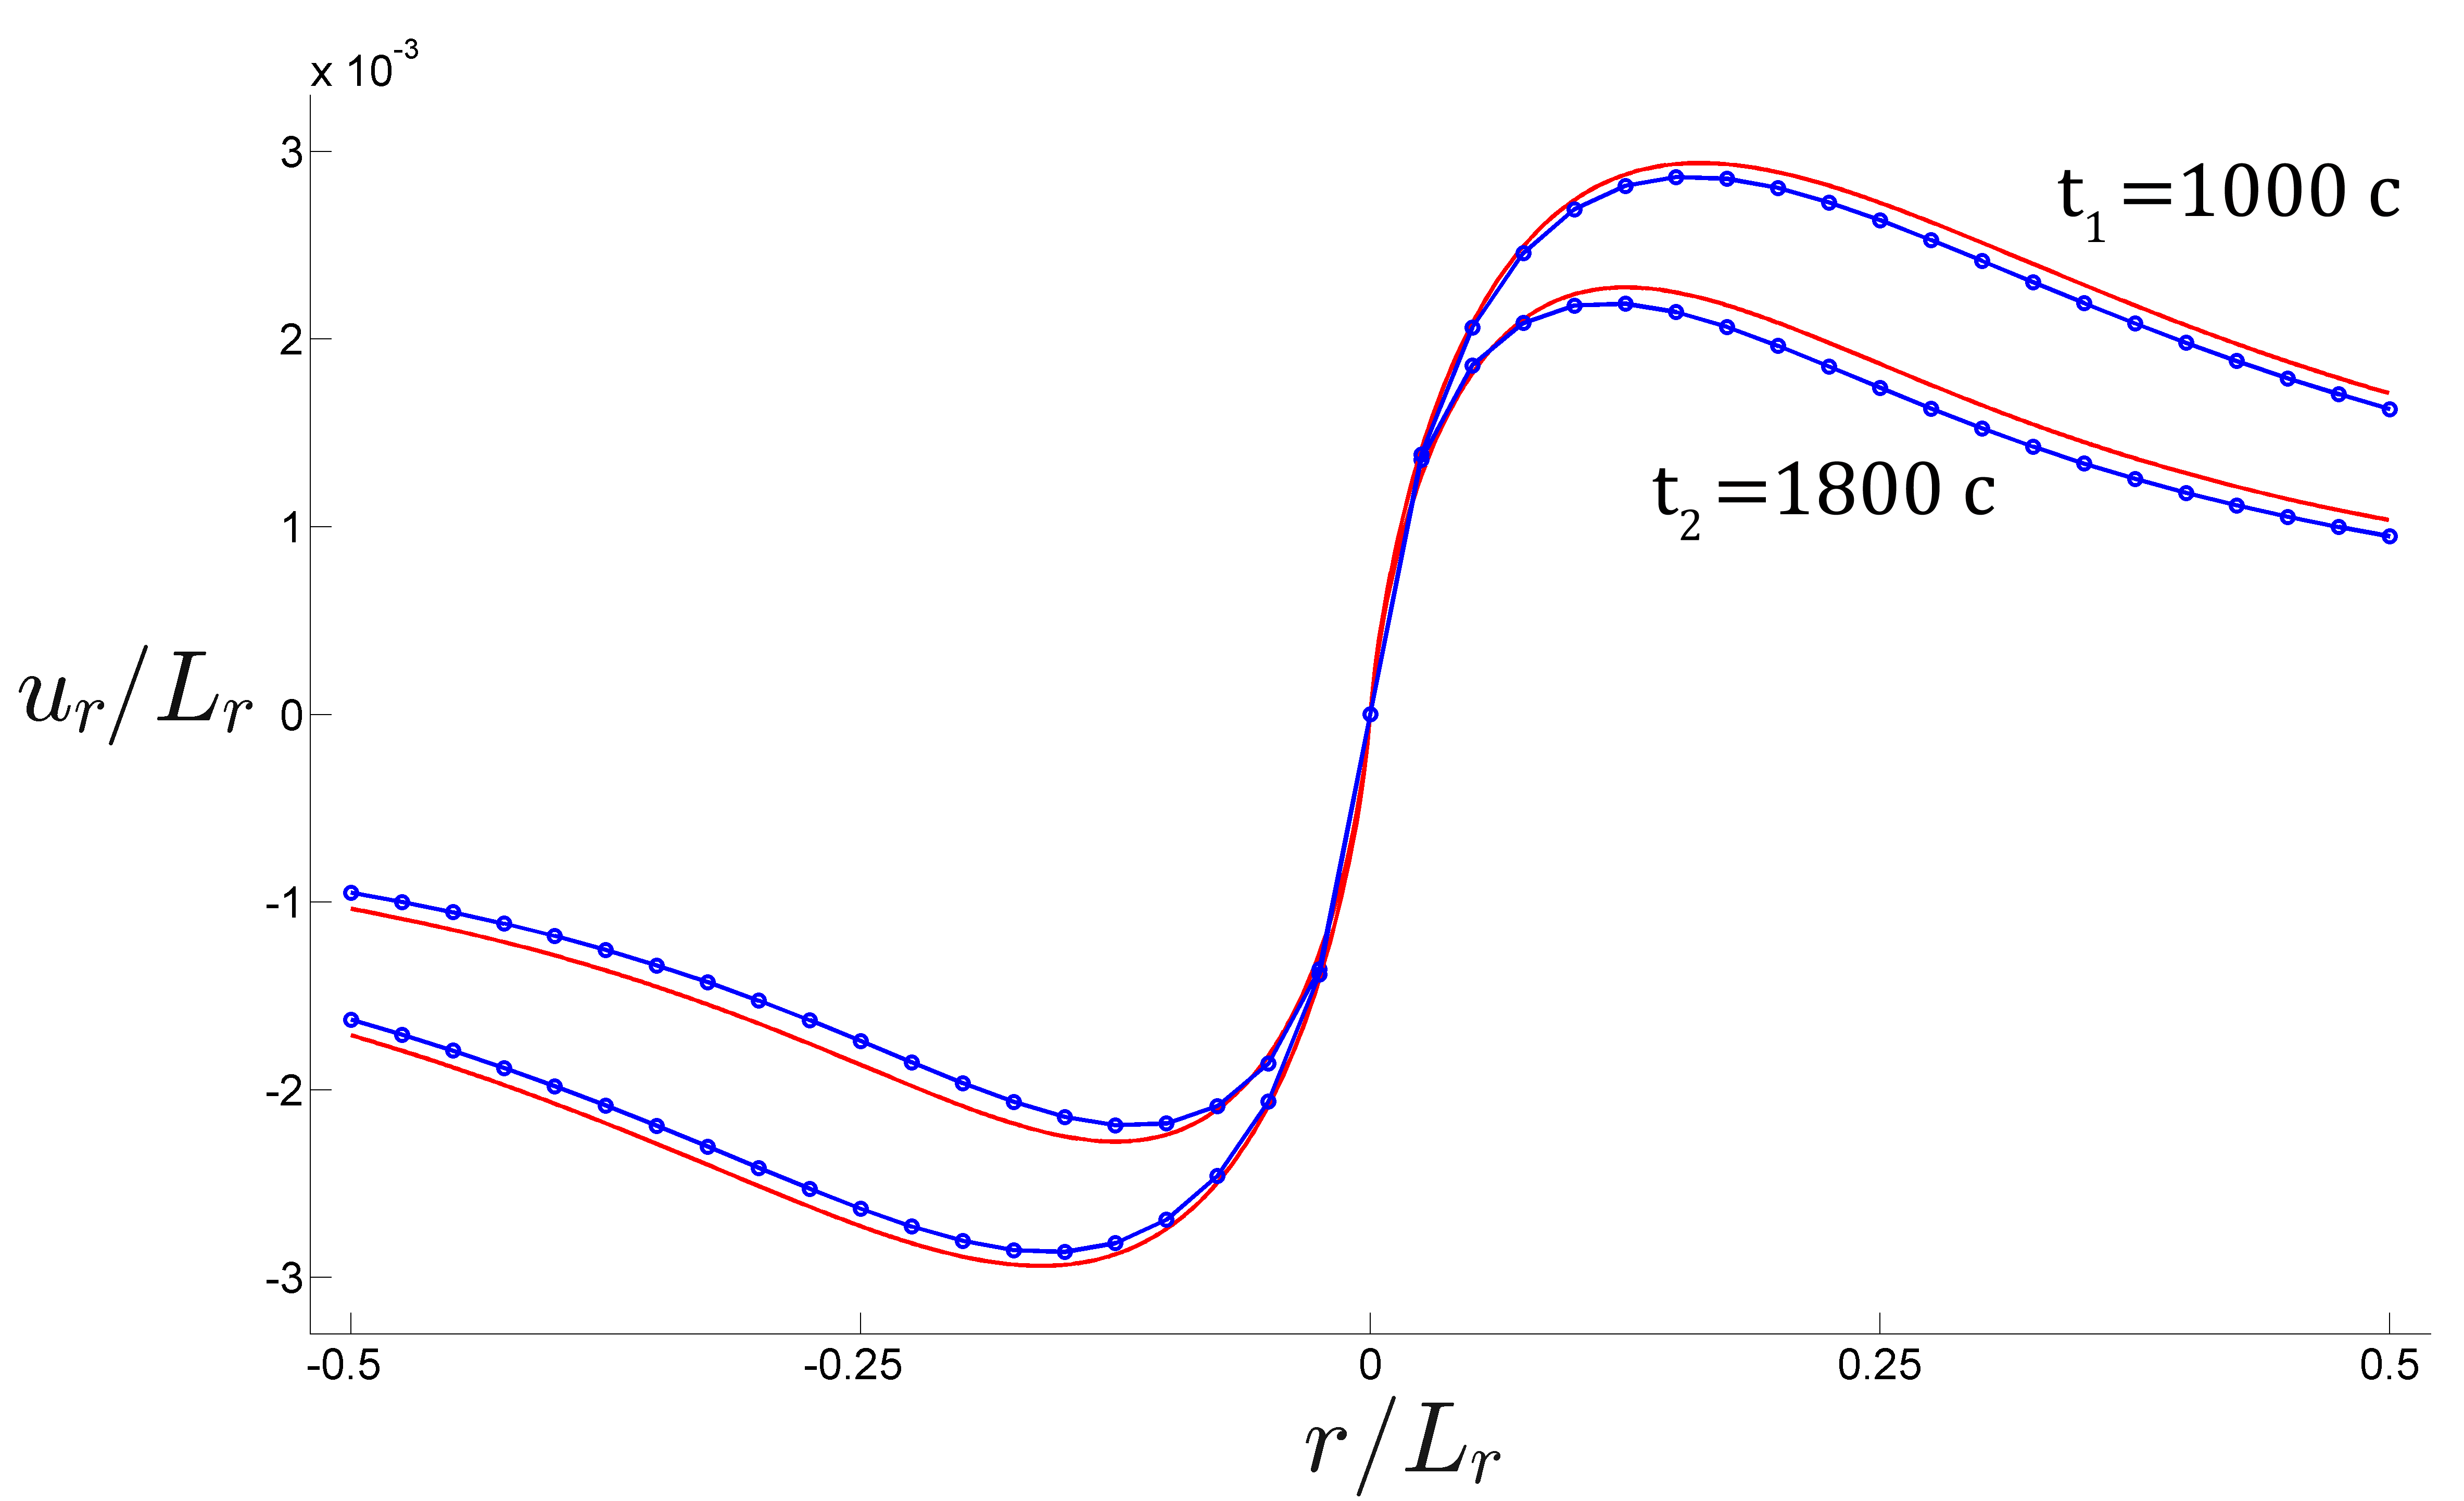
\includegraphics[width=0.98\textwidth]{figs/disp_const_line_source2.png}
%   \caption{ Нормированное перемещение в различные моменты времени: красным
% цветом показано аналитическое решение, синим – результаты расчета}
%   \label{fig::disp_const_line_source}
% \end{figure}

%\newpage
\subsection{Задача консолидации Терцаги}

Одной из классических задач пороупругости, для которых
известно аналитическое решение, является классическая одномерная задача консолидации Терцаги~\cite{terzaghi_1996}.

Рассмотрим насыщенную пороупругую область с линейными размерами $L_x$,
$L_y$, $L_z$. Верхняя граница резервуара имеет координату $z=0$,
нижняя~-- $z = L_z$.  Нижняя и боковые границы являются
непротекаемыми, при этом нижняя стенка закреплена, а боковые стенки
могут деформироваться только в вертикальном направлении. Верхняя
граница является проницаемой, к ней прикладывается сжимающее
напряжение величиной $T_z = -\sigma_0$, что приводит к деформации
пороупругой среды. В такой постановке задача является одномерной,
решение решение не зависит от $x$ и $y$.  Схематично постановка задачи
представлена на рис.~\ref{fig:terzaghi}.

%
\begin{figure}[h!]
\centering
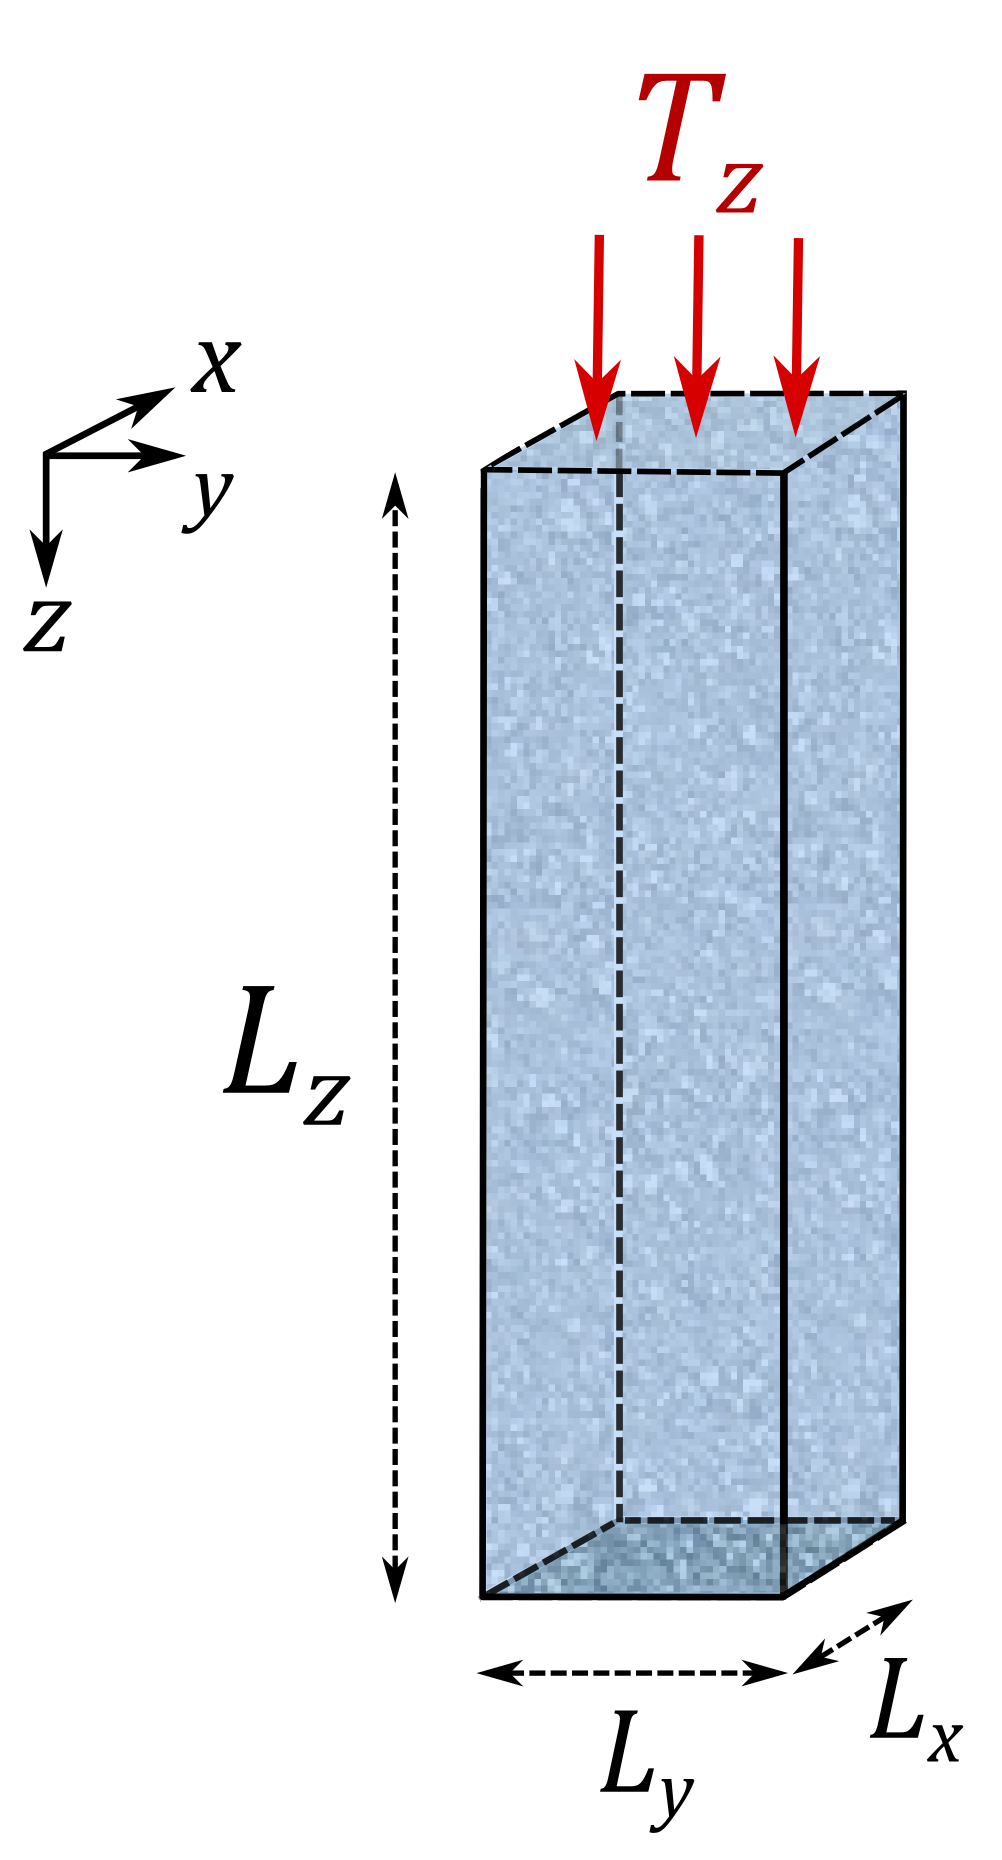
\includegraphics[width=0.35\textwidth]{./figs/terzaghi.png}
\caption{Схематичный вид задачи Терцаги.}\label{fig:terzaghi}
\end{figure}
% 

Граничные условия в одномерной постановке ставятся следующим образом:
%
\begin{equation}
\begin{aligned}
\label{eq:bcTer}
%
& z = 0:   & &\sigma_{zz}(0,t) = -\sigma_0, & &p(0,t) = 0, \\
%
& z = L_z: & &u_z(L_z,t) = 0, & &\cfrac{\partial p}{\partial z} = 0.
%
\end{aligned}
\end{equation}
%

Начальные условия после мгновенного нагружения задаются в виде
%
\begin{equation}
%\begin{split}
\label{eq:icTer}
%
u_z(z,0^+) \equiv u_0 = \sigma_0 (L_z - z) / K_v^{(u)},\quad
p(z,0^+) \equiv p_0 = \gamma \sigma_0.
%
%\end{split}
\end{equation}

Аналитическое решение задачи может быть записано как~\cite{wang_2000}:
%%
\begin{multline}
\label{eq:Pter}
%
p(z,t) = p_0 - p_0 \sum \limits_{m=0}^{\infty} \left(-1\right)^m
%
\left[   
\text{erfc} \cfrac{(2m+1)L_z - (z-L_z)}{\sqrt{4ct}} \right. \\ \left. + \; \text{erfc} \cfrac{(2m+1)L_z+(z-L_z)}{\sqrt{4ct}}
\right],
%
\end{multline}
%%

%%
\begin{multline}
\label{eq:Uter}
%
u_z(z,t)= u_0 + c_m\gamma\sigma_0 
%
\left[
(L_z-z) - \cfrac{8L_z}{\pi^2} \sum \limits_{m=0}^{\infty} \cfrac{1}{(2m+1)^2} \right. \\
\left. \cdot \exp \left( \cfrac{-(2m+1)^2\pi^2 c t}{4L_z^2}  \right) 
\cdot \cos \left( \cfrac{(2m+1)\pi z}{2 L_z}  \right)
\right].
%
\end{multline}
%%

Здесь
%
\begin{gather*}
%
\gamma = \cfrac{B(1+\nu_u)}{3(1-\nu_u)}, \quad
c_m\gamma = \cfrac{\nu_u-\nu}{2G(1-\nu)(1-\nu_u)}, \\[7pt]
%
c = \cfrac{2kG(1-\nu)(\nu_u-\nu)}{\mu b^2 (1-2\nu)^2(1-\nu_u)}, \quad K_v^{(u)} = \cfrac{2G(1-\nu_u)}{1-2\nu_u}.
%
\end{gather*}
%

В качестве данных для сравнения используются нормированные значения $\overline{p}$ и
$\overline{u}_z$:
%
\begin{equation*}
%
\overline{p} = \cfrac{p}{p_0}, \quad \overline{u} = \cfrac{u_z}{L_z}, \quad 
\overline{z} = \cfrac{z}{L_z}, \quad \overline{\tau} = \cfrac{ct}{L_z^2}.
%
\end{equation*}
%
%\vspace{5mm}

Конкретные значения используемых для расчетов параметров приведены в табл.~\ref{tab:terzaghi}.
%
%%
\begin{table}[h!]
\centering
%
\renewcommand{\arraystretch}{1.5}
\renewcommand{\tabcolsep}{6 pt} 
\begin{tabular}{|c|c|c|c|c|c|c|}
\hline
$L_z$ & $L_x$ & $L_y$ & $\sigma_0$ & $t_{\text{start}}$ & $t_{\text{end}}$ & $\Delta t$\\
\hline
 $15.0$ м & $1.0$ м & $1.0$ м & $1.0$ КПа & $0.0$ с & $1500.0$ с & $1.0$ с\\
\hline
\end{tabular}
%
\caption{Параметры для численного расчета задачи Терцаги.}\label{tab:terzaghi}
\end{table}
%%
%

Для численных расчетов использовалась тетраэдральная сетка, состоящая из 
$N_{nodes} = 1600$ узлов и $N_{elems} = 5346$ прямоугольных тетраэдров со сторонами
$h_x = h_y = 0.3333$ м, $h_z = 0.1515$ м. В отличие от представленной выше постановки задачи и аналитического решения
для нее при проведении расчетов в программном комплексе начало координат и ориентация оси $Oz$ были выбраны другими.
В силу этого при сравнении с аналитическим решением полученное численное решение при необходимости нормировалось соответствующим образом.

%
\begin{figure}[t!]
\centering
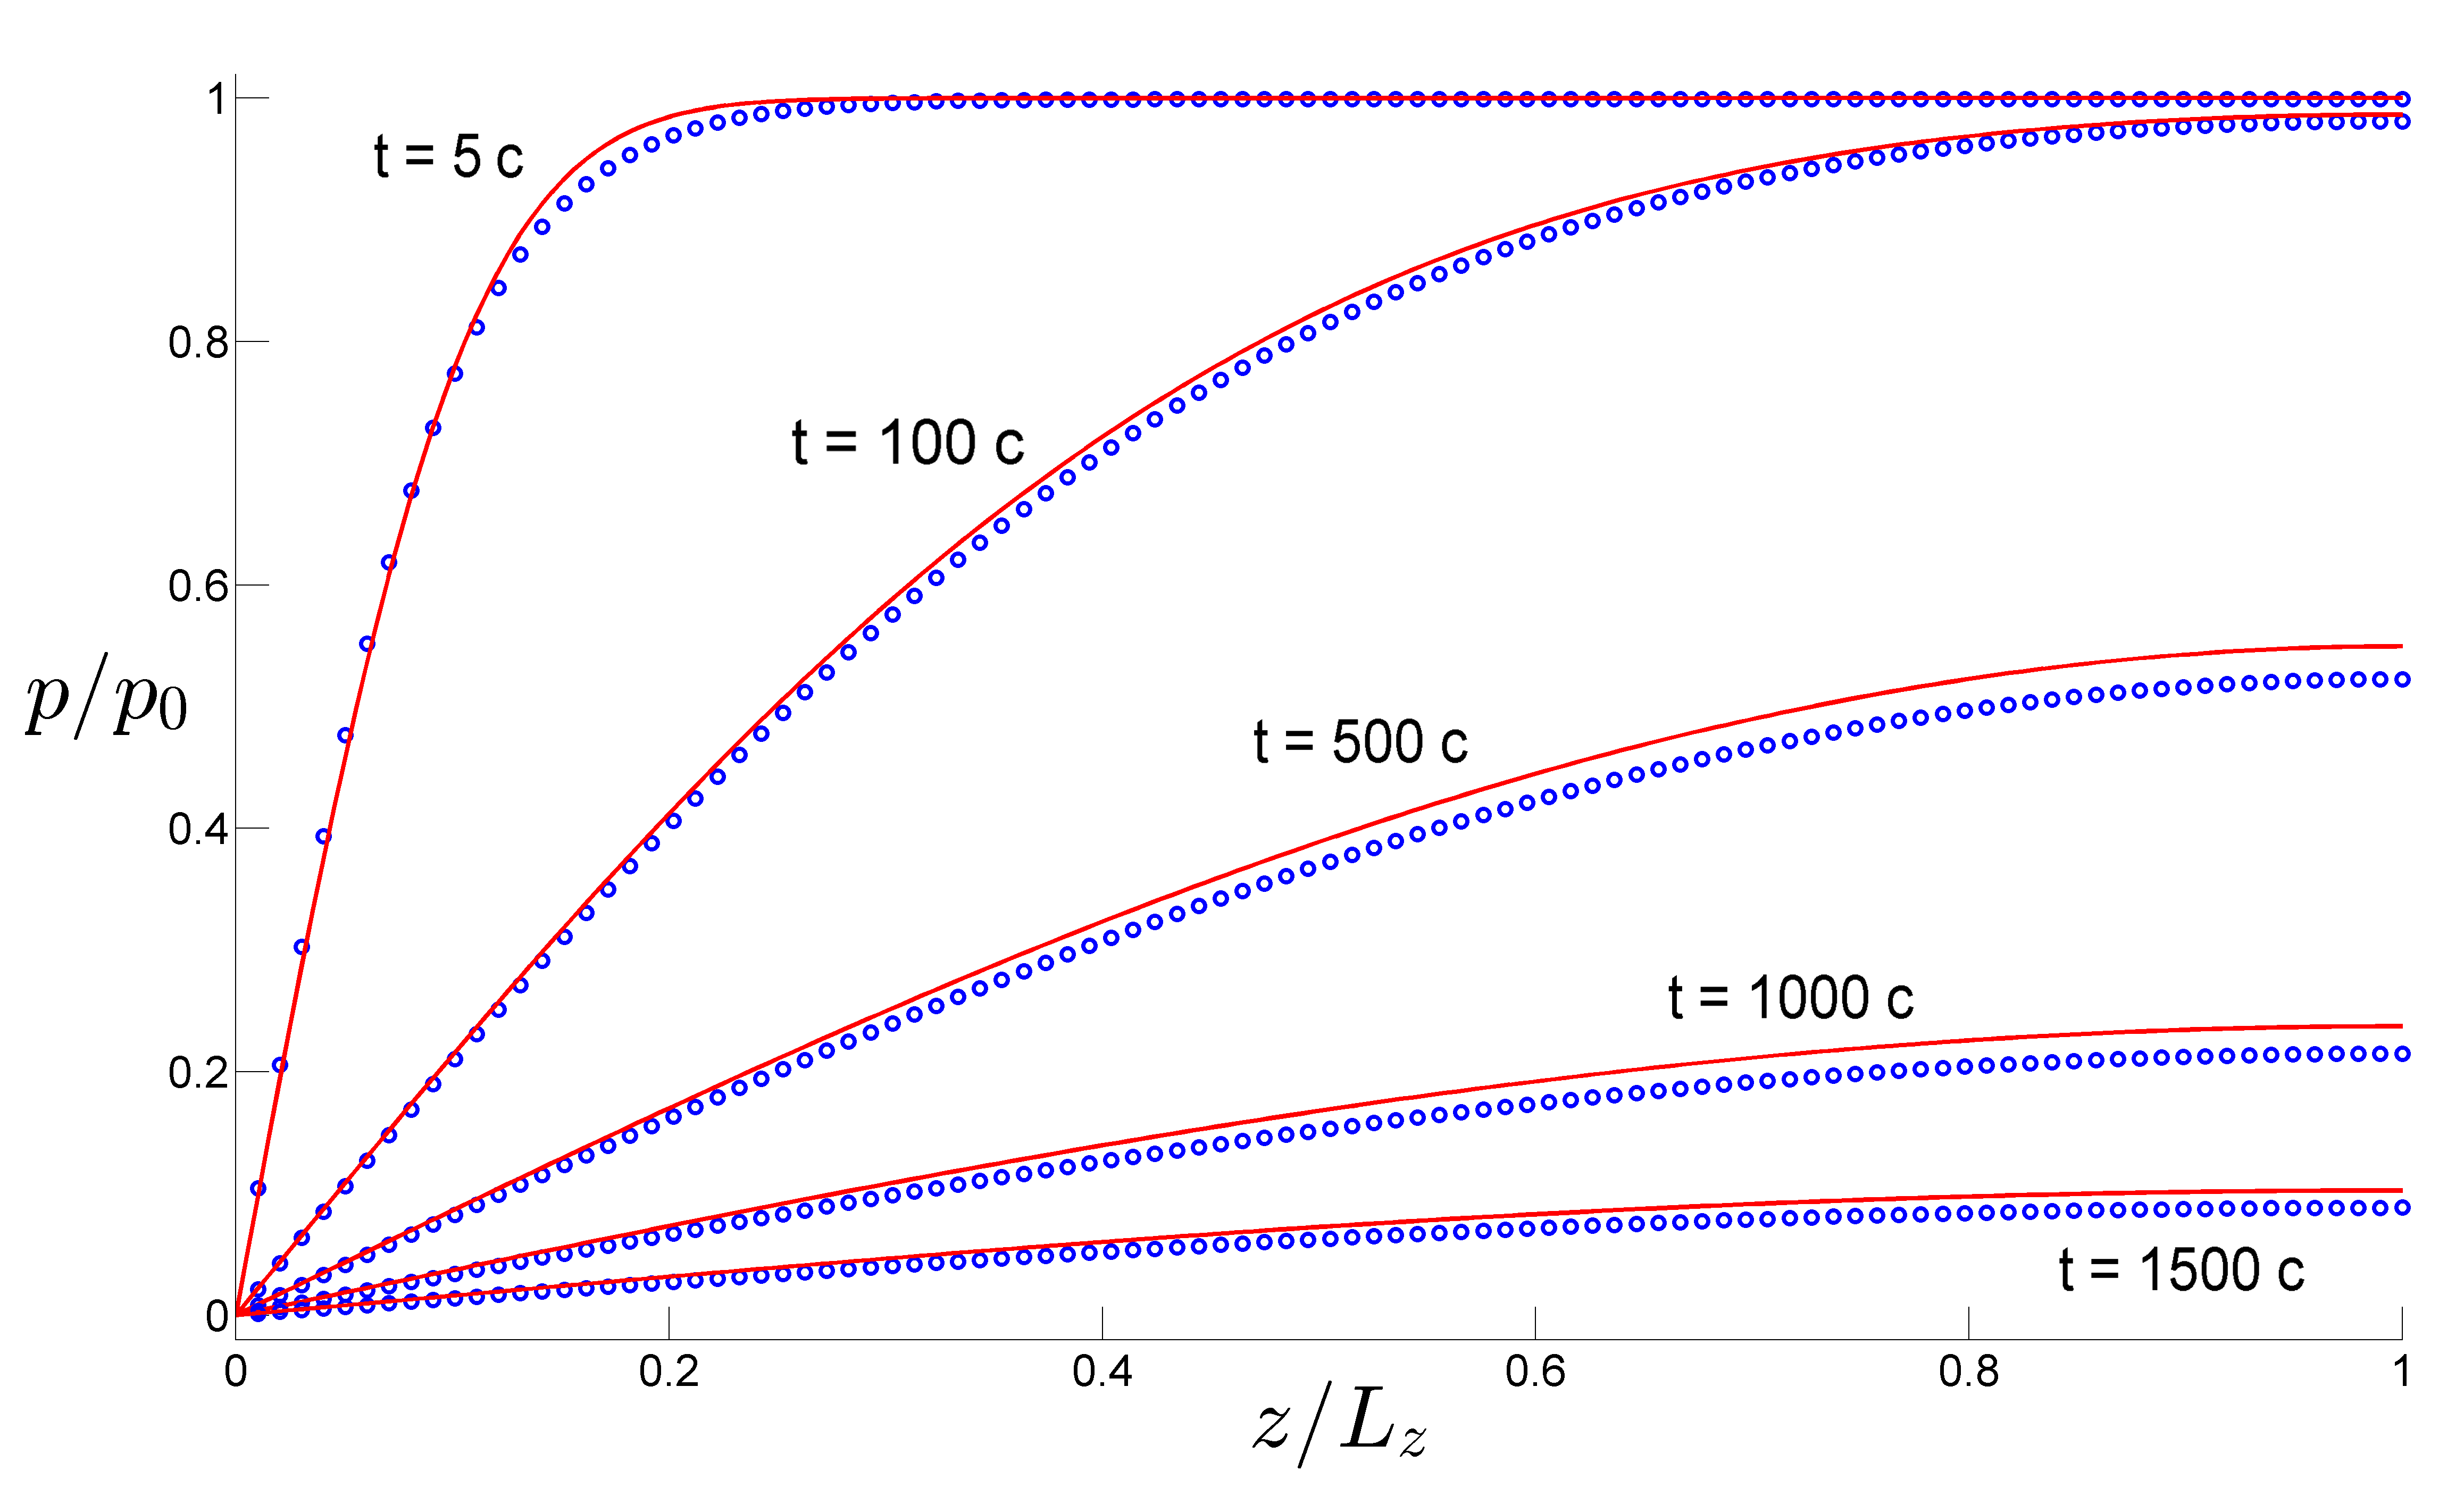
\includegraphics[width=0.9\textwidth]{./figs/pp0Ter.png}\\
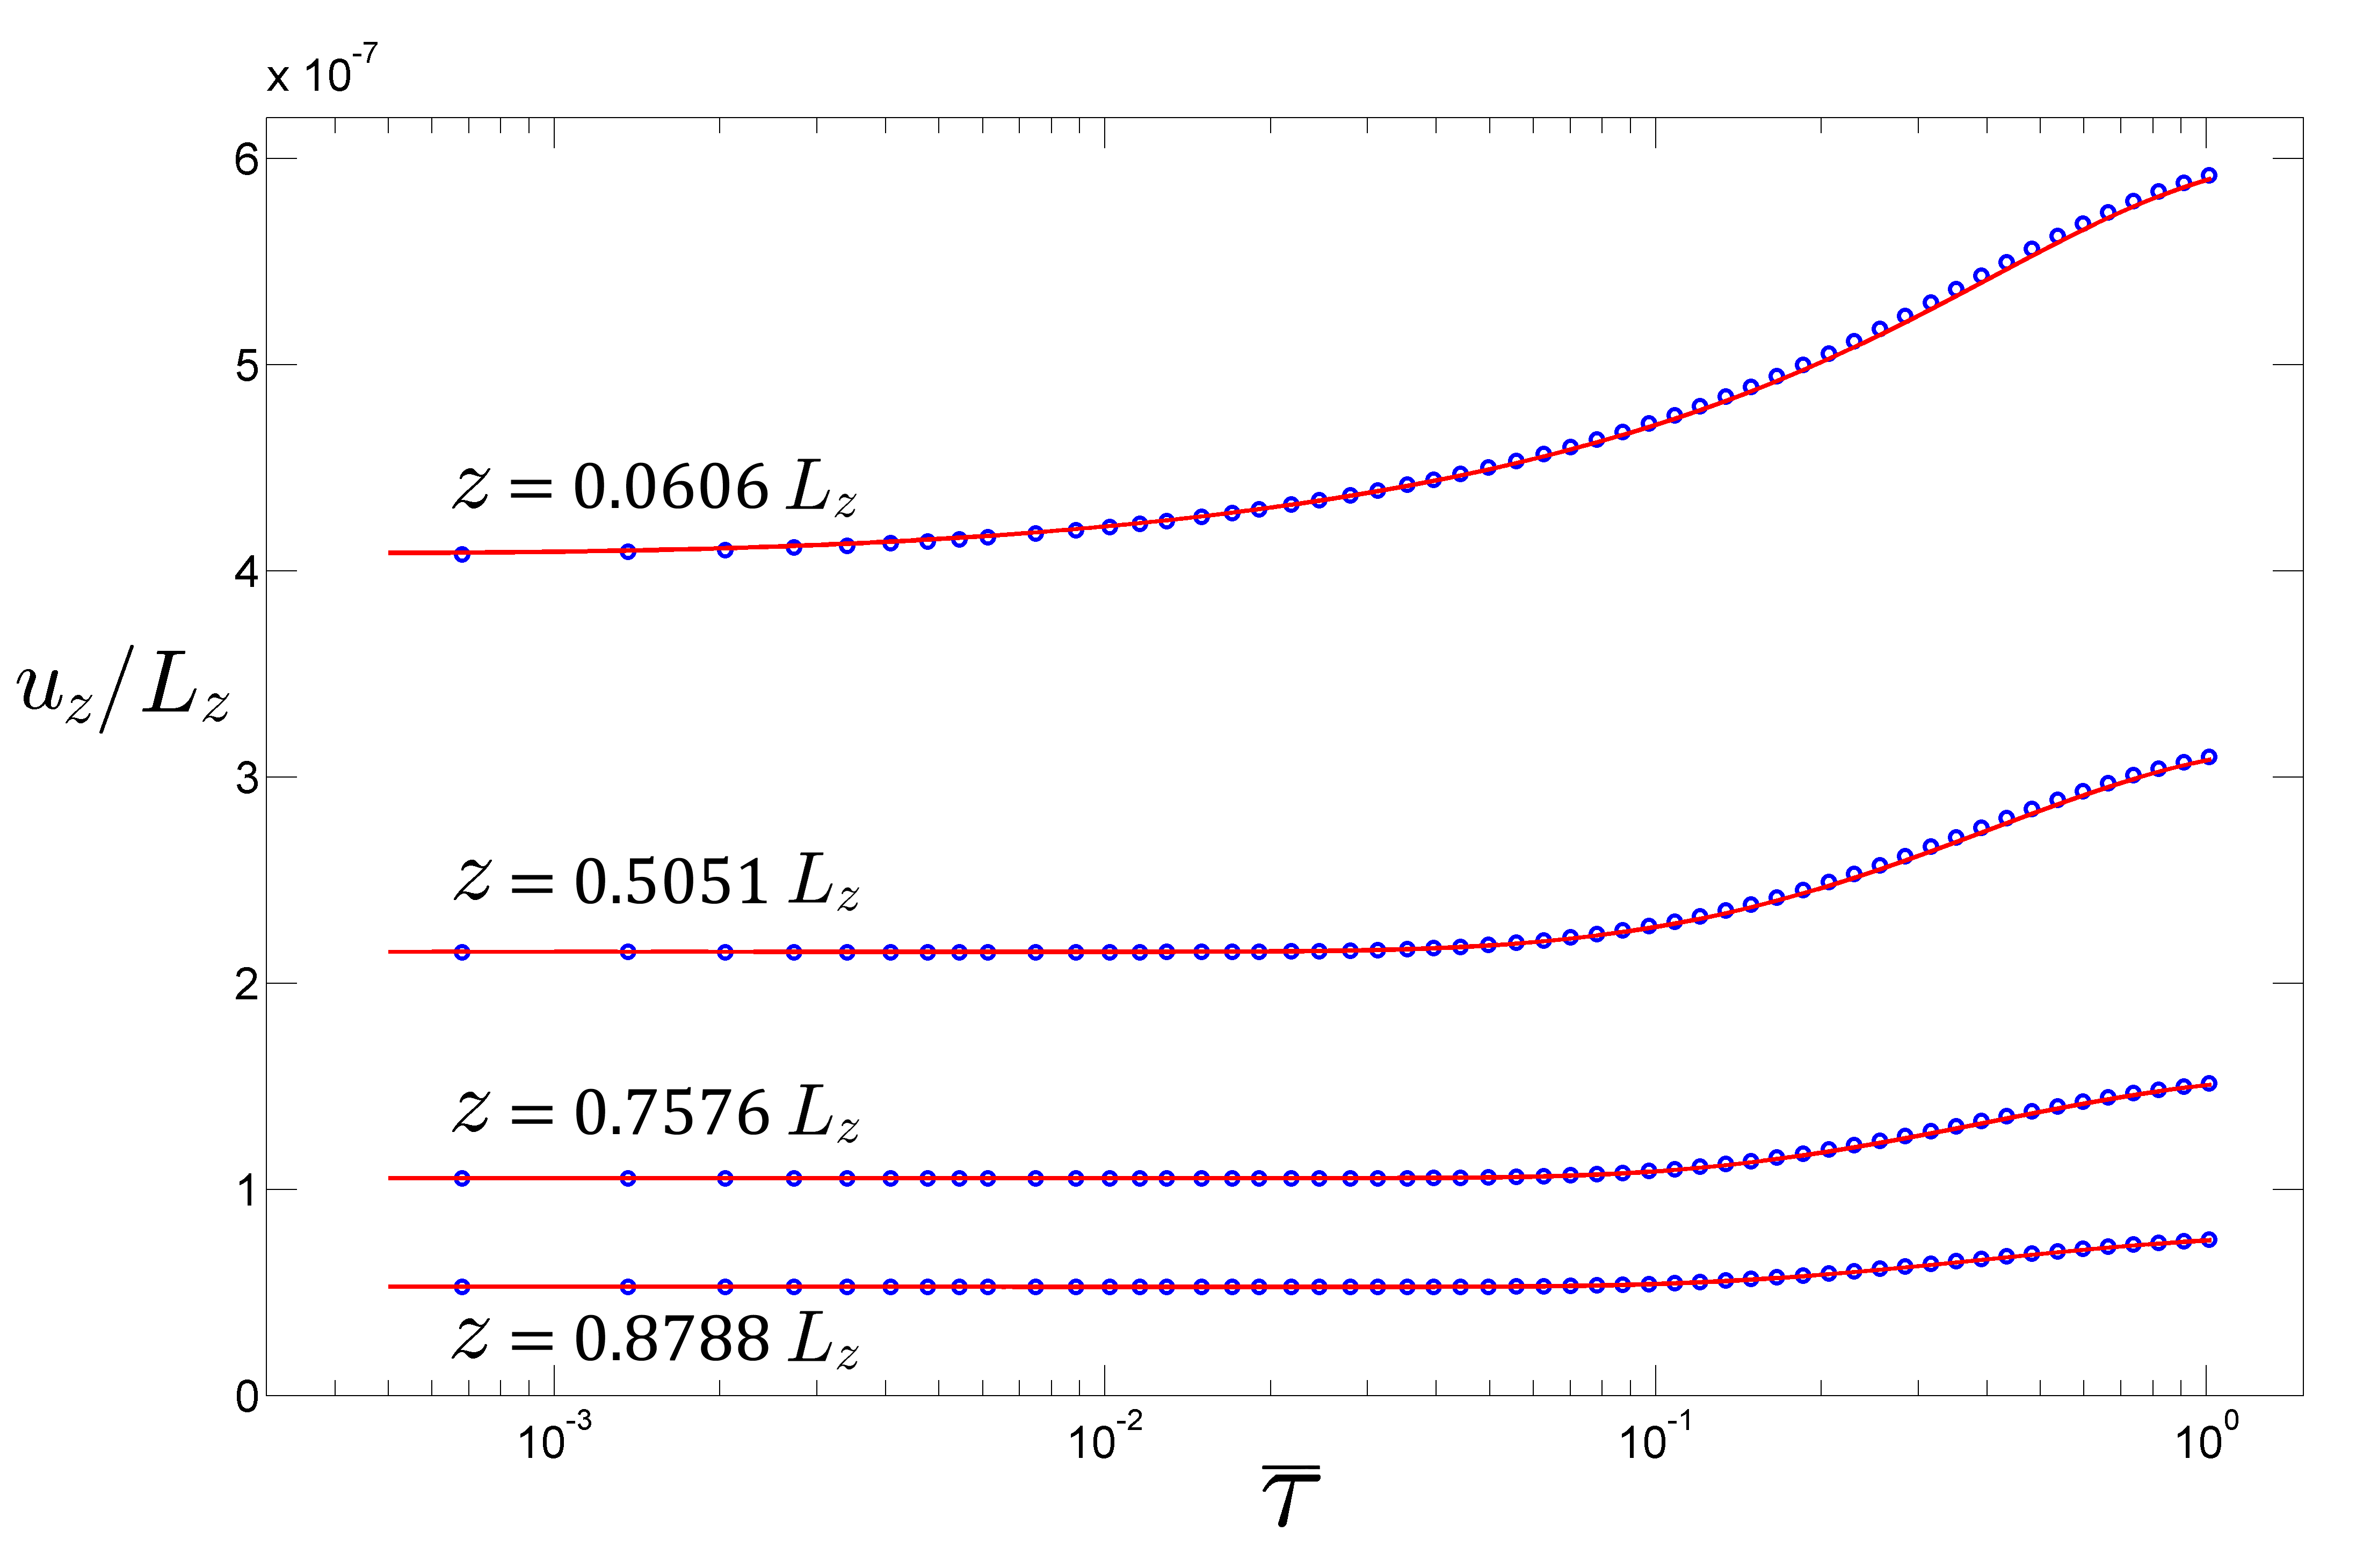
\includegraphics[width=0.9\textwidth]{./figs/uu0Ter.png}
\caption{ Задача консодидации Терцаги. Нормированное давление (вверху) и перемещение (внизу) в
  различные моменты времени: красным цветом показано
аналитическое решение, синим~--- результаты расчета.}\label{fig:terp}
\end{figure}
% 
% \begin{figure}[h!]
% \centering
% 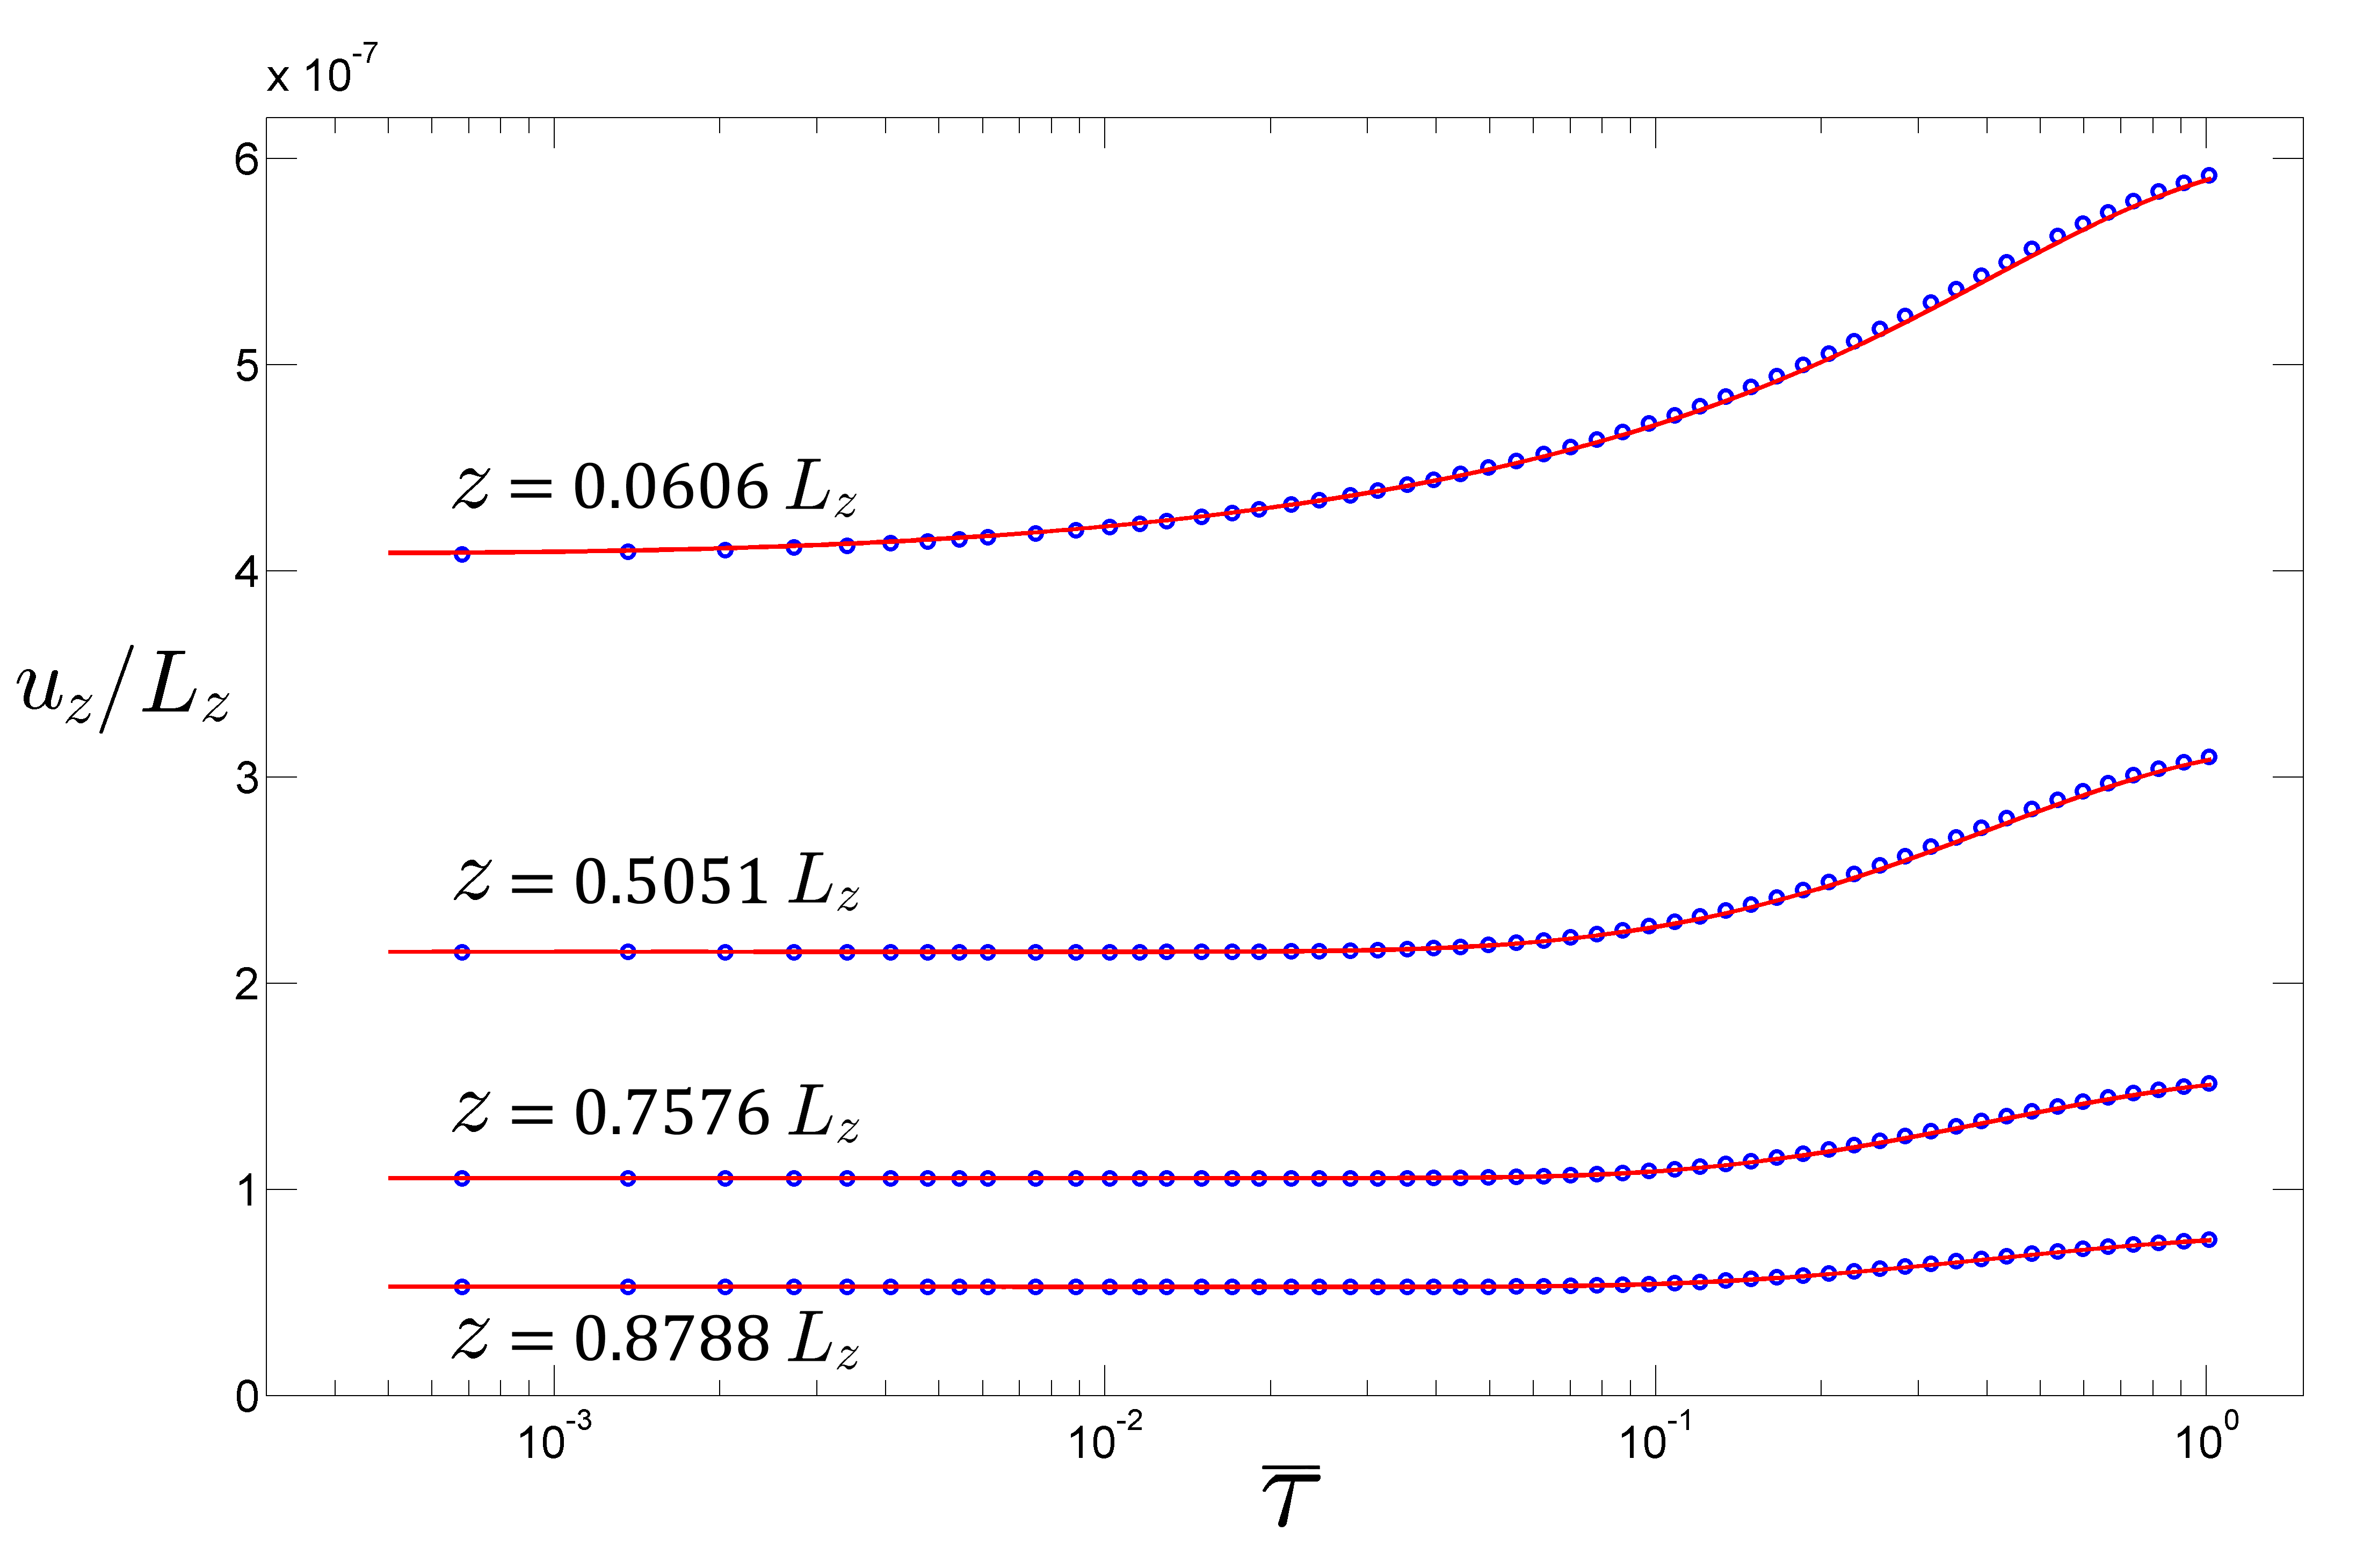
\includegraphics[width=0.9\textwidth]{./figs/uu0Ter.png}
% \caption{Нормированное перемещение в различные моменты времени: красным цветом показано
% аналитическое решение, синим~--- результаты расчета.}\label{fig:teru}
% \end{figure}
% 
 
На рис.~\ref{fig:terp} (вверху) показано распределение нормированного на начальную нагрузку $p_0$ давления $p$ в зависимости
от нормированной глубины $z/L_z$ в последовательные моменты времени $t = 5, \; 100, \; 500, \; 1000, \; 1500$ c.
Рис.~\ref{fig:terp} (внизу) демонстрирует нормированное на высоту колонны $L_z$
перемещение $u_z$ в зависимости от безразмерного времени $\overline{\tau}$ для нескольких выделенных глубин
$z/L_z = 0.0606, \; 0.5051, \; 0.7576, \; 0.8788$. На обоих рисунках красным цветом показано
соответствующие аналитическое решение, синим~-- результаты численного расчета, при этом данные для анализа брались в центральных точках области,
равноудаленных от боковых границ резервуара.
Как видно из представленных рисунков, расчеты продемонстрировали хорошее совпадение с аналитическими
данными. Также в качестве иллюстрации на рис.~\ref{fig:terpp}
%и~\ref{fig:teruu} 
приведены полученные в расчетах размерные распределения
полей давления $p$ и перемещения $u_z$ в последовательные моменты времени
$t = 100, \; 500, \; 1000, \; 1500$ c.

\begin{figure}[t!]
\centering
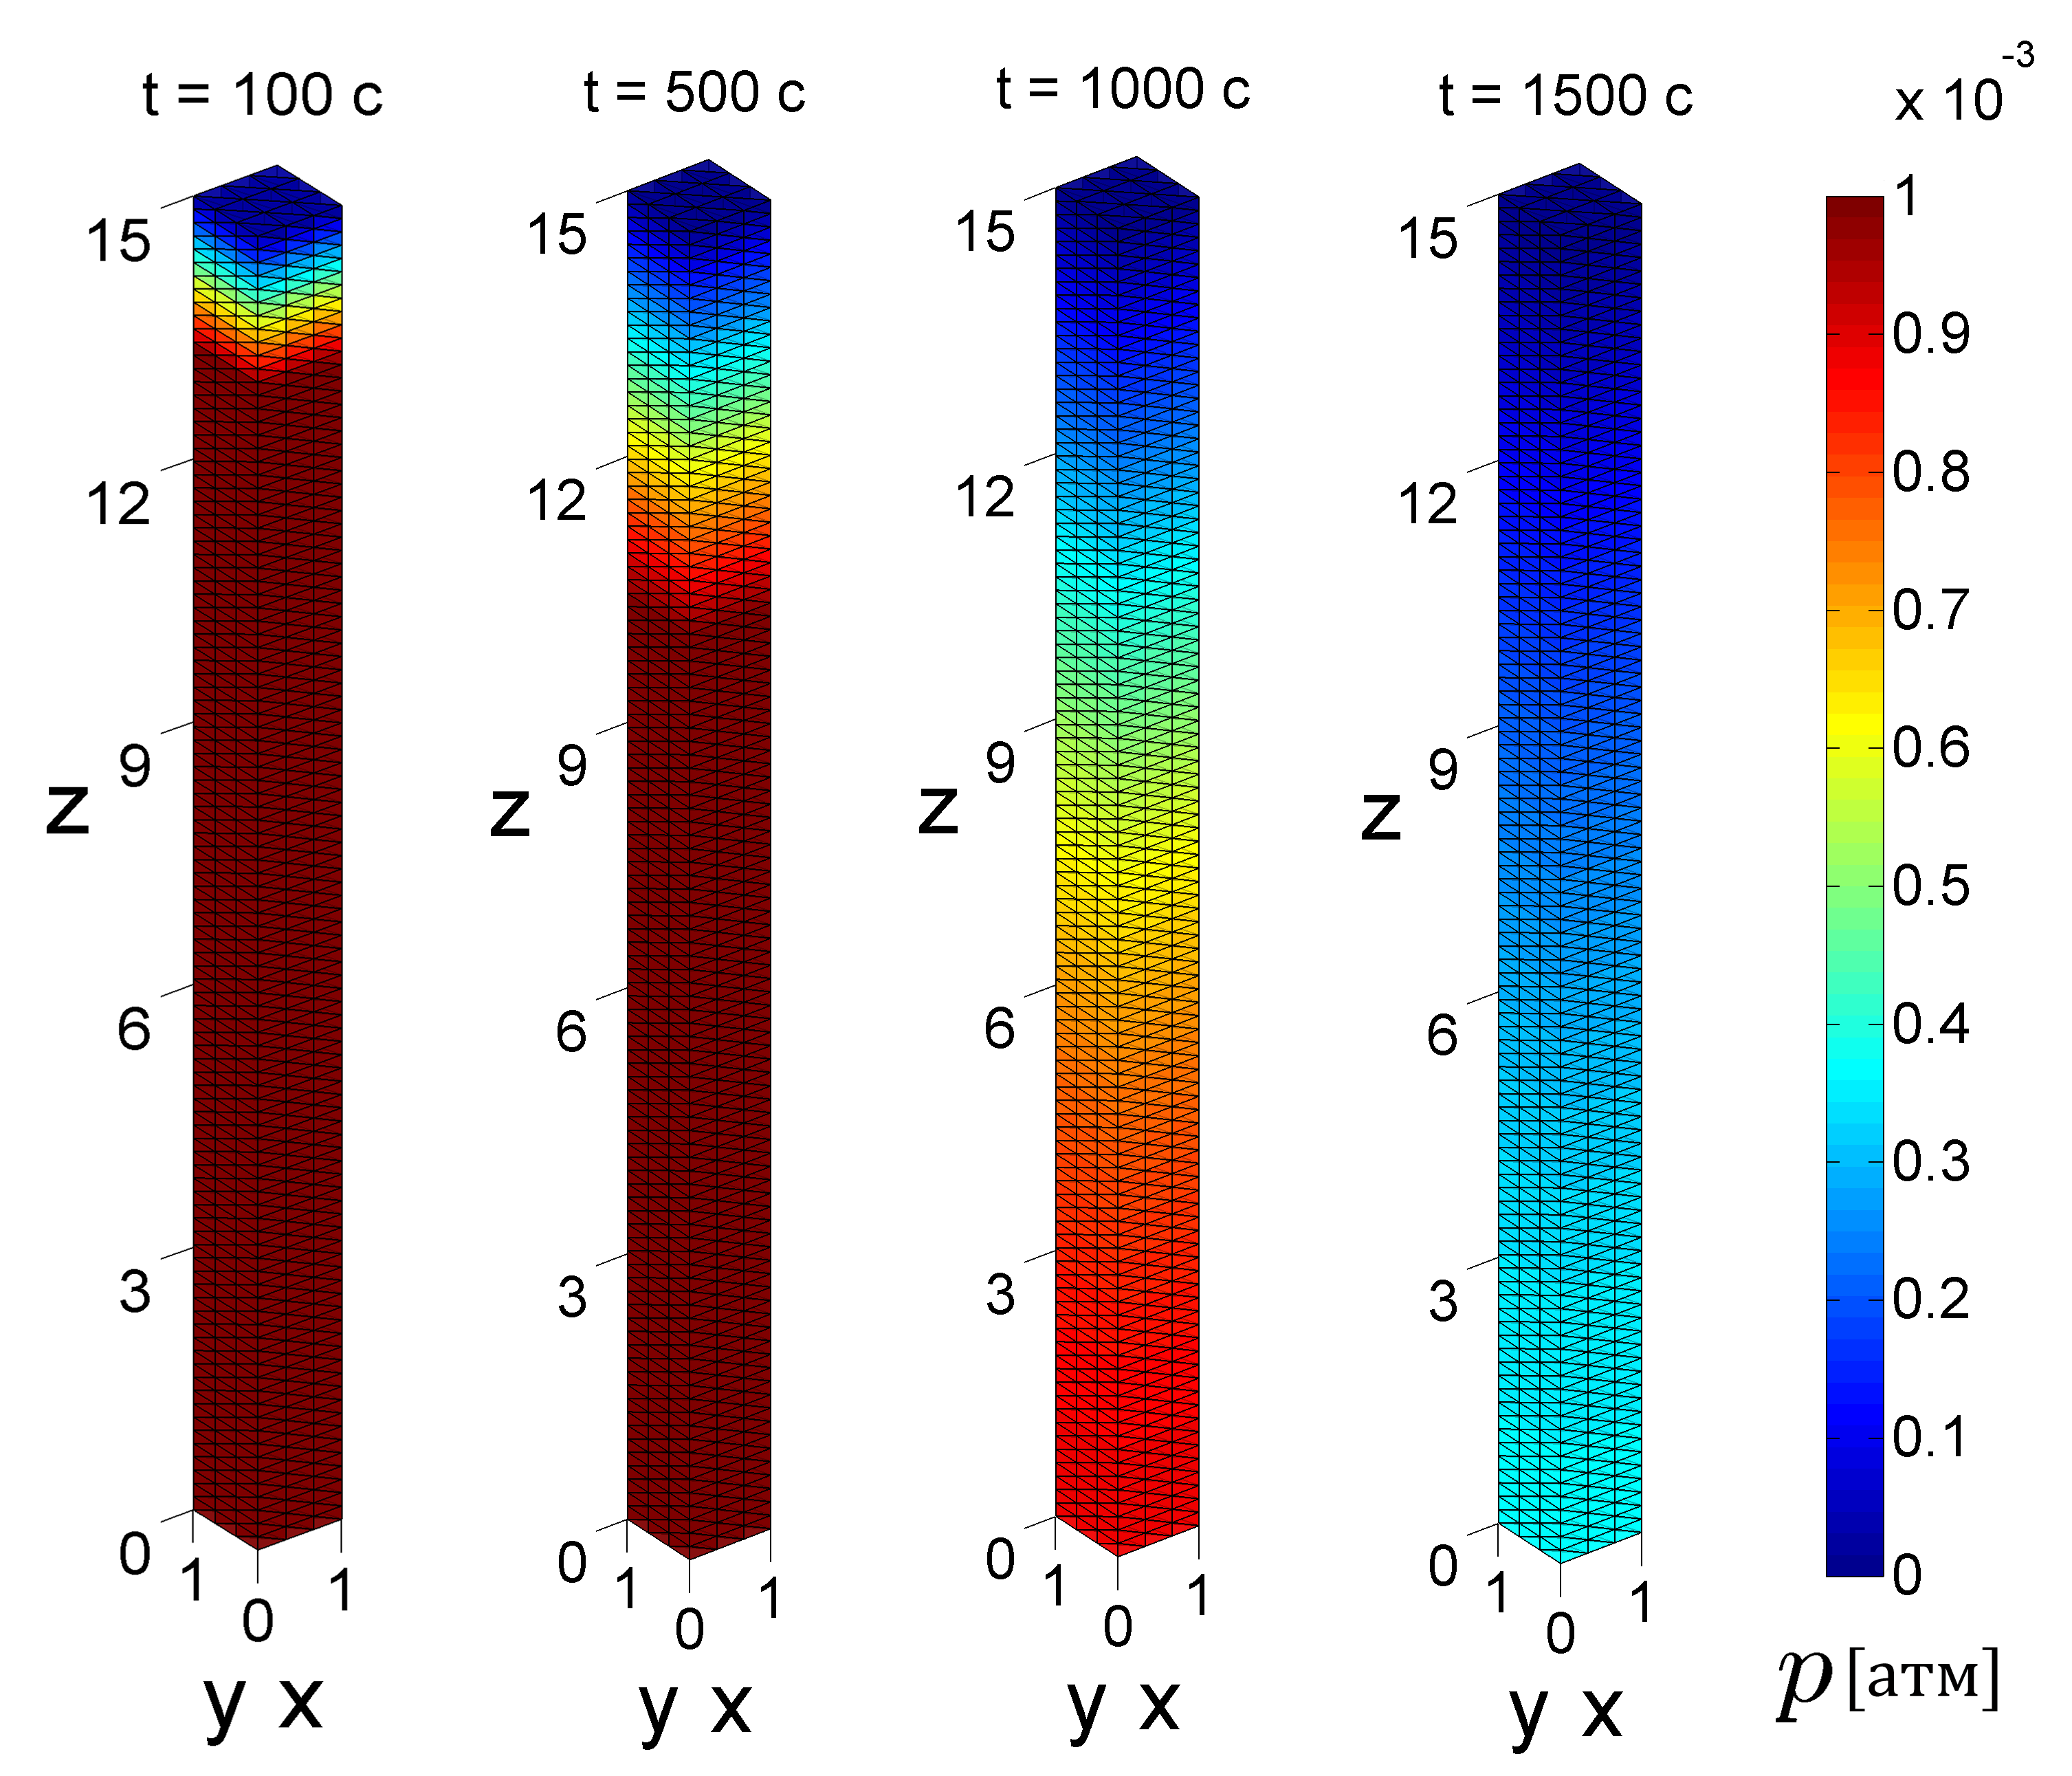
\includegraphics[width=0.75\textwidth]{./figs/pp1Ter.png}\\
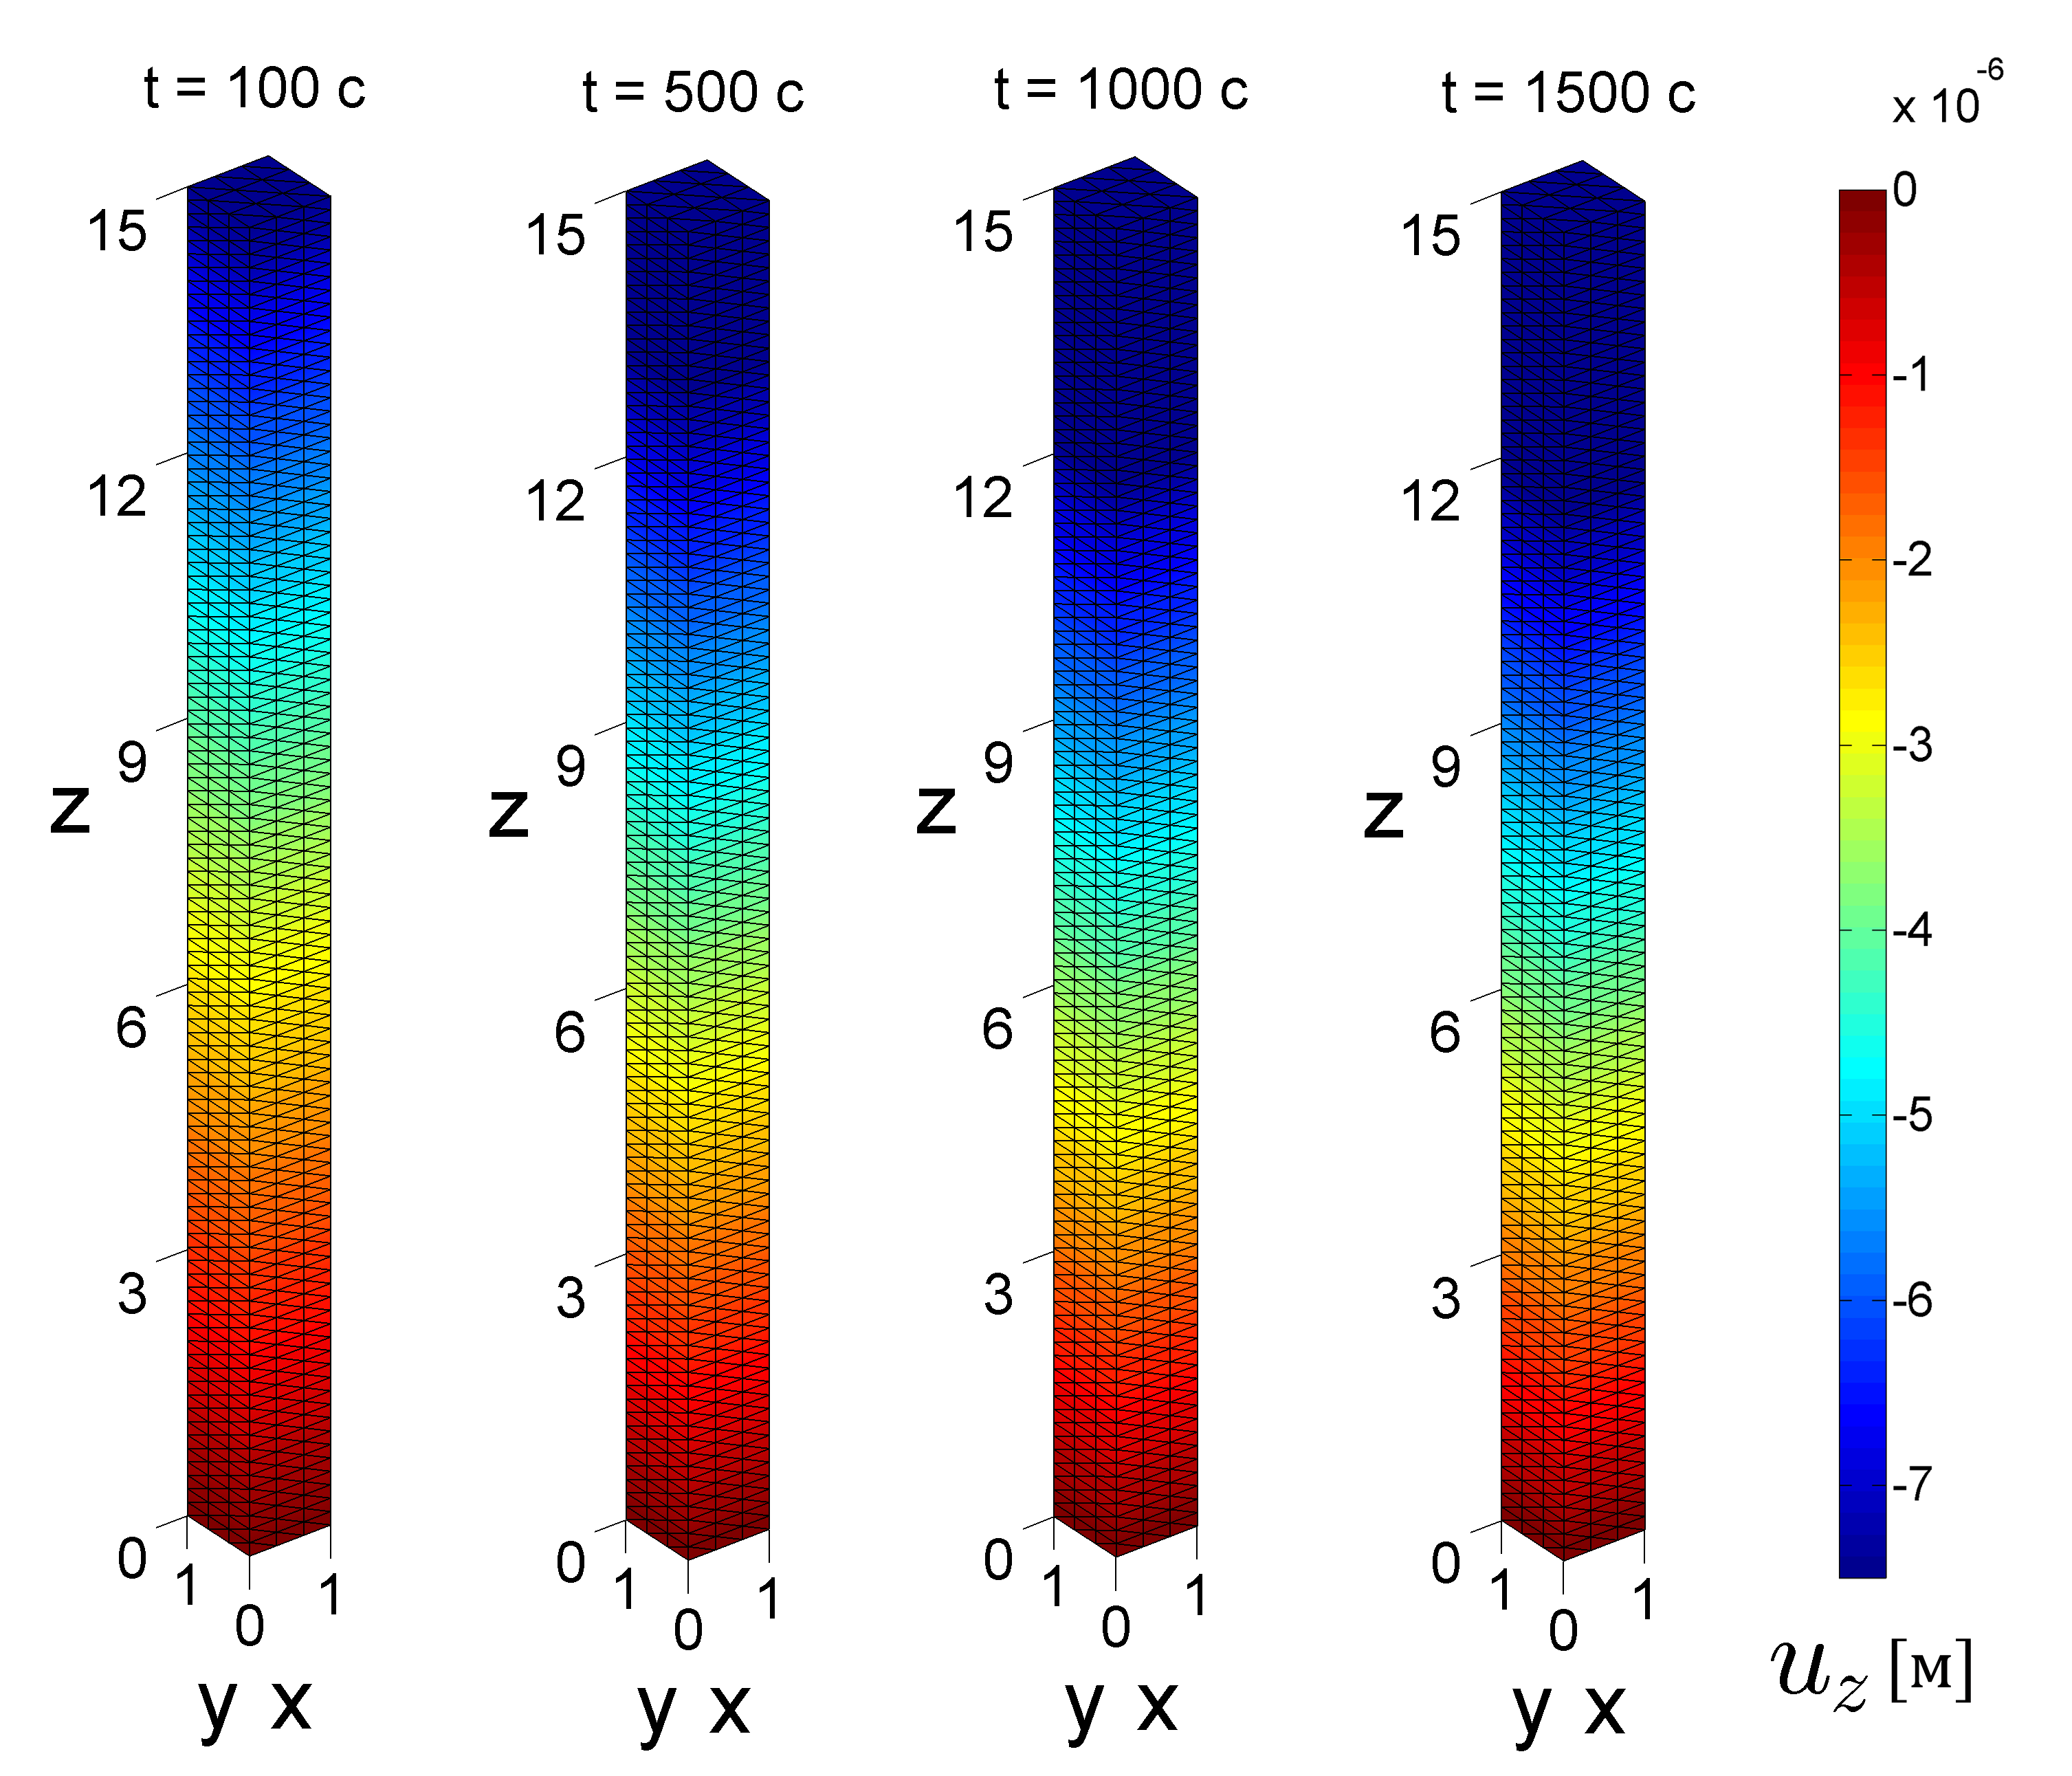
\includegraphics[width=0.75\textwidth]{./figs/uu1Ter.png}
\caption{ Задача консодидации Терцаги. Распределение давления (вверху) и перемещений $u_z$ (внизу) в 
последовательные моменты времени.}\label{fig:terpp}
\end{figure}
%
% \begin{figure}[b!]
% \centering
% 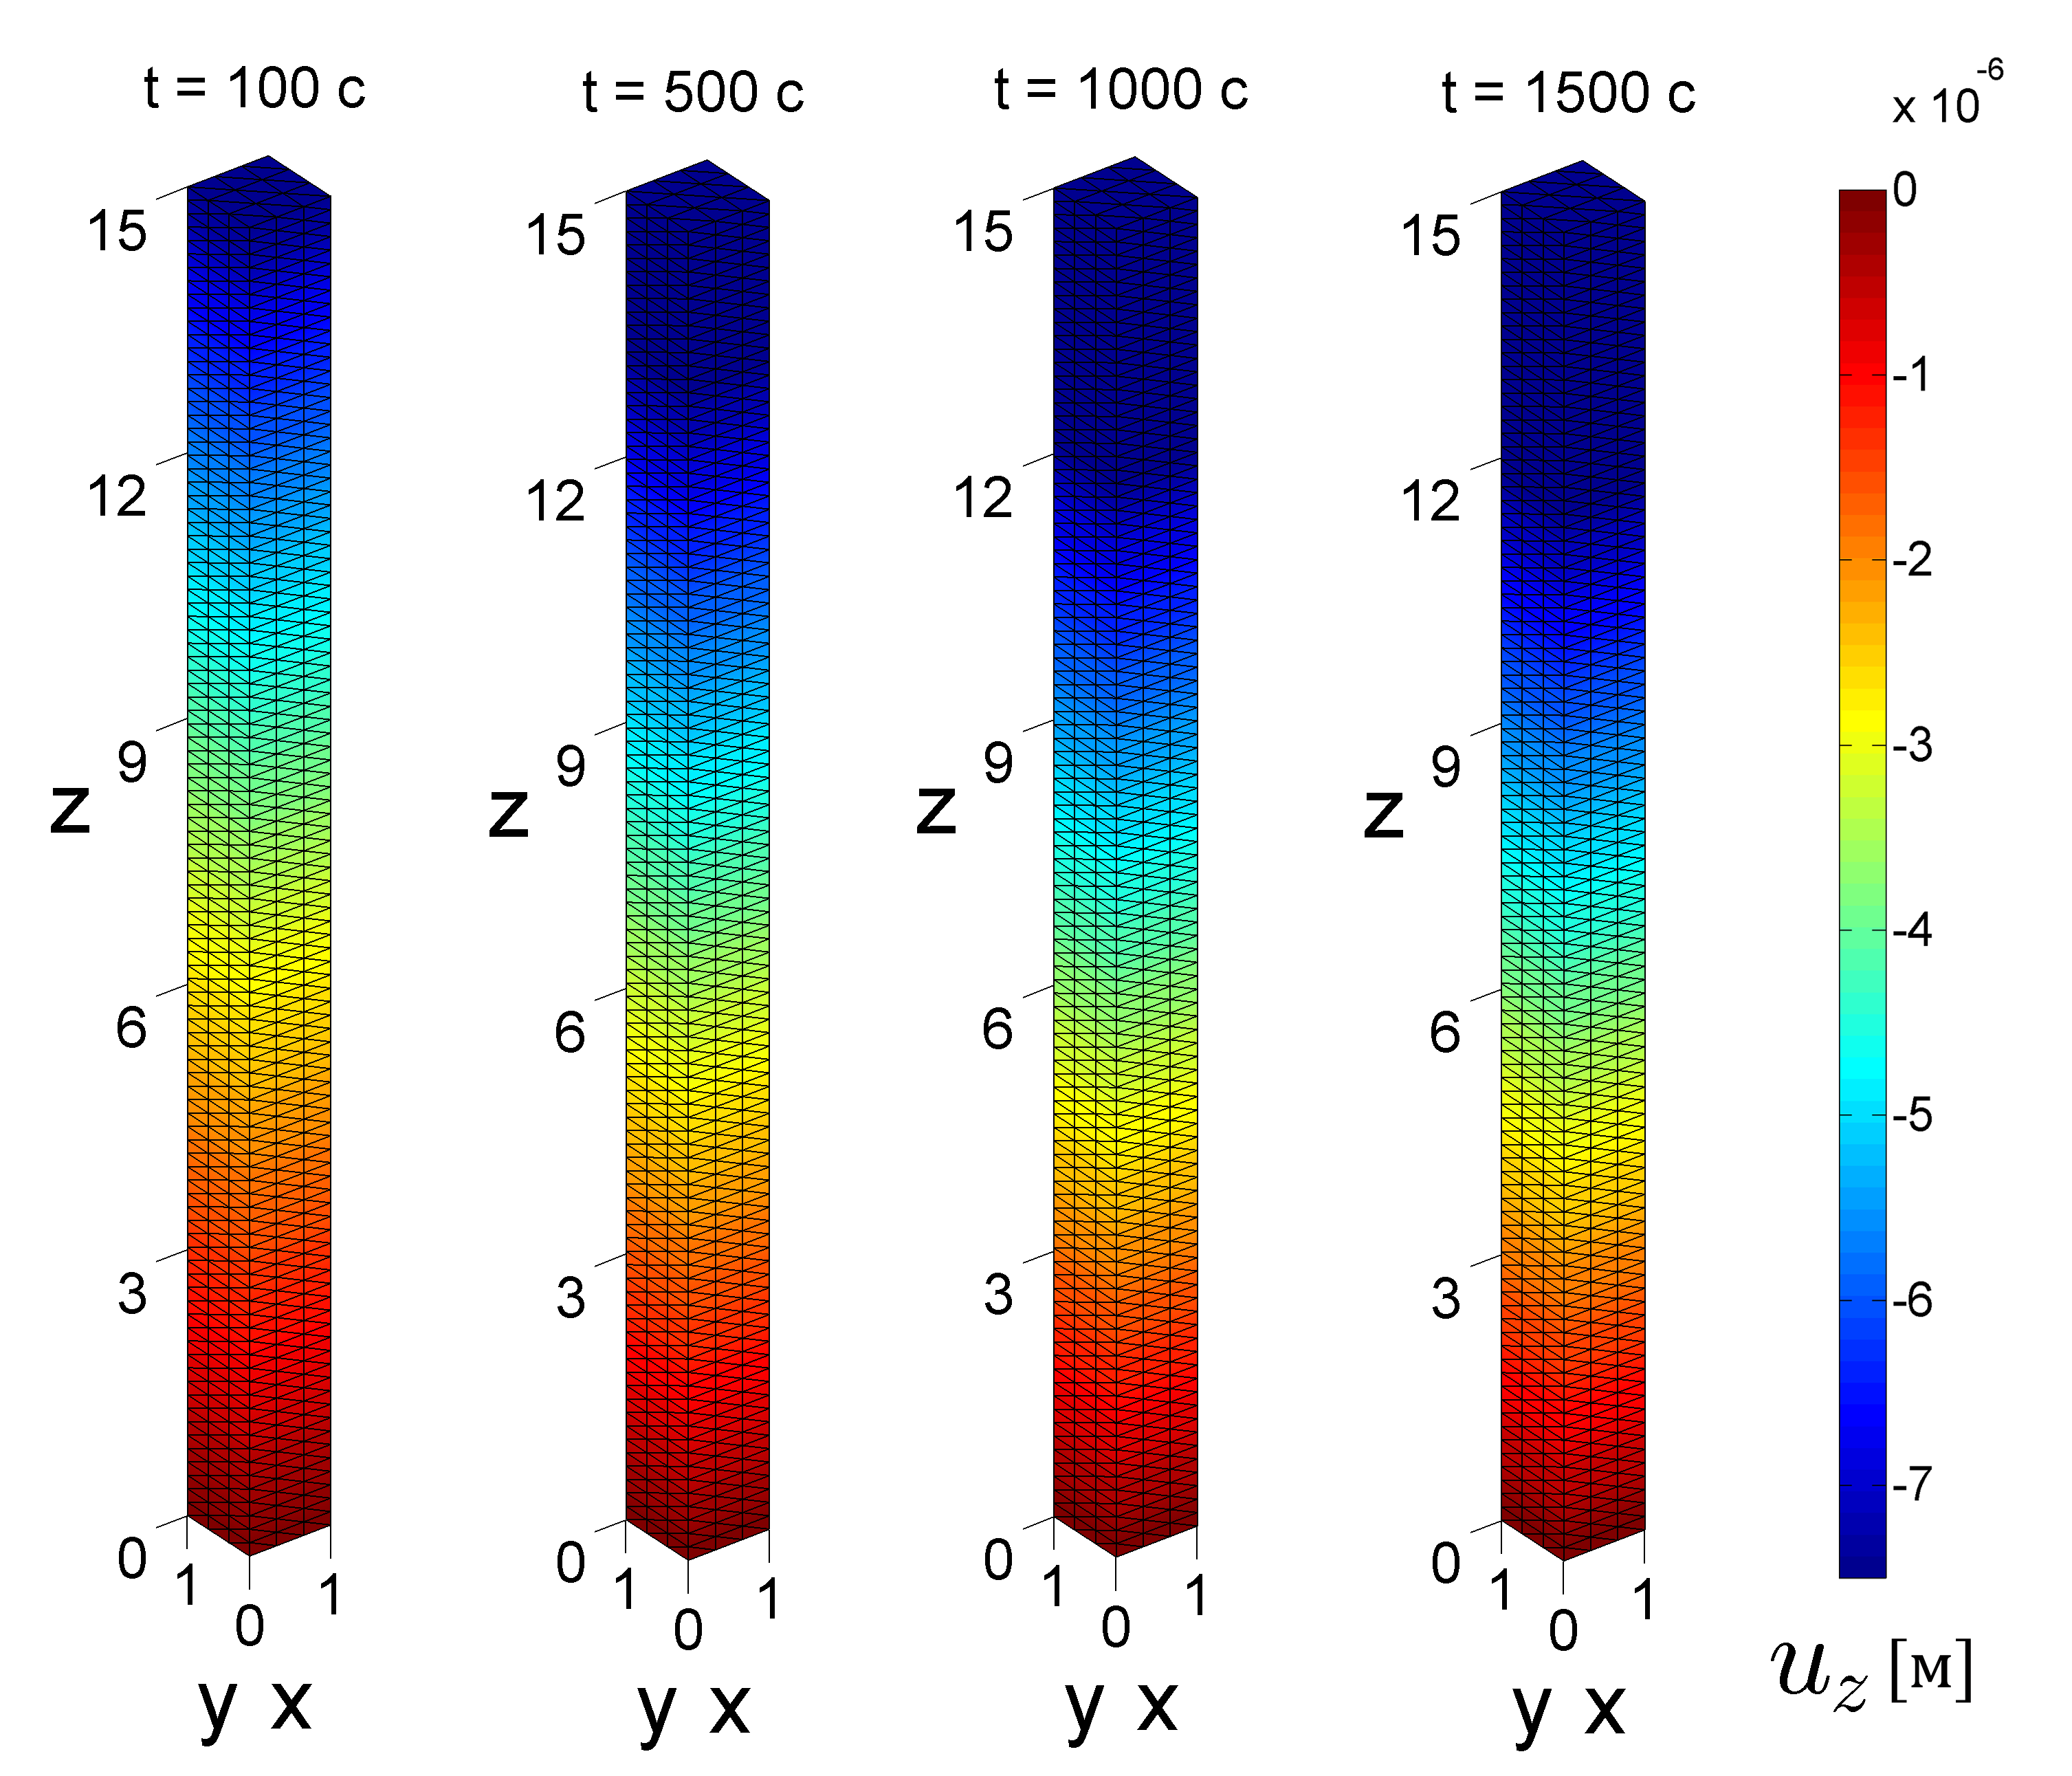
\includegraphics[width=0.95\textwidth]{./figs/uu1Ter.png}
% \caption{Распределение перемещений $u_z$ в последовательные моменты времени.}\label{fig:teruu}
% \end{figure}
% 

%\clearpage

\subsection{Задача Манделя}

Мандель в своей работе~\cite{mandel_1953} продемонстрировал классический
пример немонотонного поведения распределения порового давления по времени при недренированном нагружении
в условиях плоских деформаций.
В оригинальной постановке задача ставилась следующим образом. Рассматривалась насыщенная пороупругая среда
с линейными размерами $2a \times 2b$, зажатая между двумя жесткими непроницаемыми пластинами.
В начальный момент времени на пластины мгновенно начинала действовать сжимающая сила $F = -2\sigma_0a$,
нормированная на единичную длину в $z$ направлении и далее не меняющаяся со временем. 
Боковые границы области полагались свободно деформируемыми и проницаемыми, в начальный момент времени
среда покоилась. 

В силу симметрии задачи в настоящей работе для численных расчетов используется одна восьмая часть резервуара,
с началом координатам в центре исходной области. Также в отличие от оригинальной постановки предполагается,
что нагружение осуществляется в плоскости $Oxz$. Схематично задача представлена на рис.~\ref{fig:mandel}.
Здесь $L_x = a$ м, $L_z = b$ м, $T_z = -\sigma_0$.
%
\begin{figure}[h!]
\centering
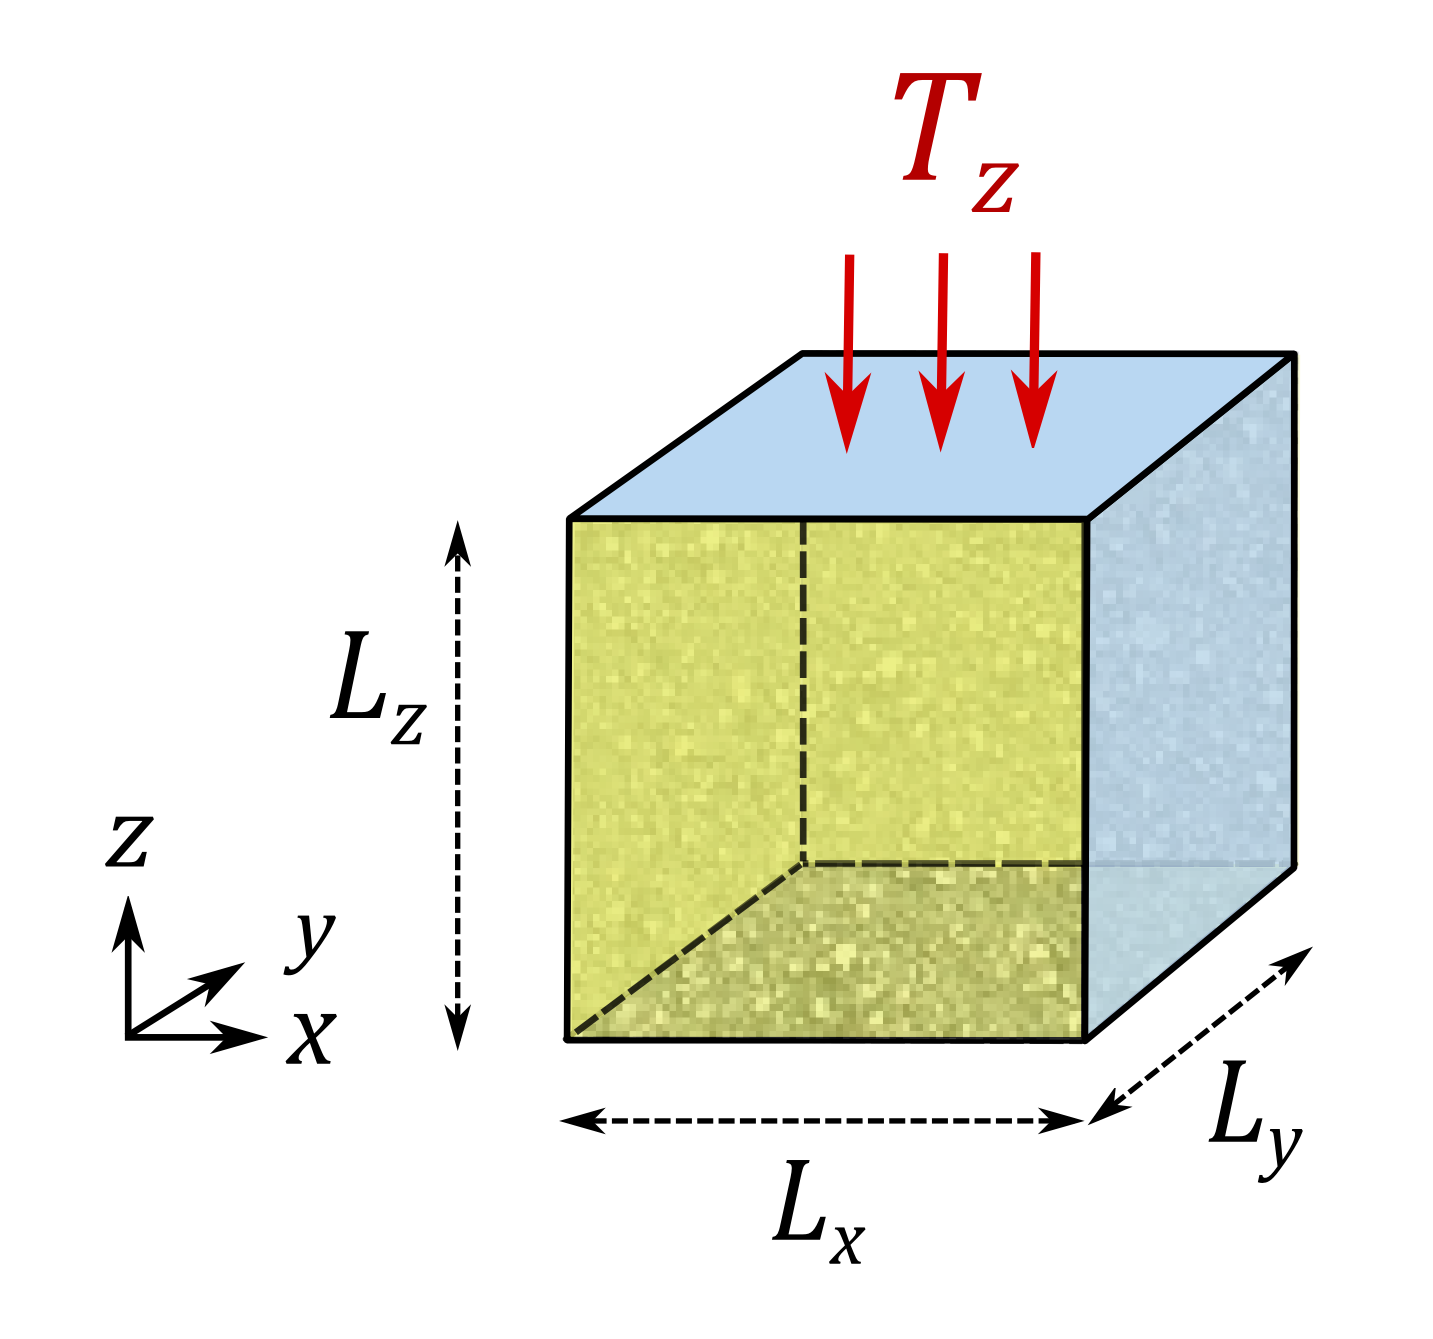
\includegraphics[width=0.65\textwidth]{./figs/mandel.png}
\caption{Схематичный вид задачи Манделя. Желтым цветом выделены плоскости
симметрии в соответствии с граничными условиями.}\label{fig:mandel}
\end{figure}
% 

Граничные условия в двумерной постановке ставятся следующим образом:
%
\begin{equation}
\begin{aligned}
\label{eq:bcMan}
%
& x = 0: & &u_x = 0, \;  \partial p / \partial x = 0, \\
& x = a: & &\sigma_{xx} = 0, \;p = 0,\\
%& y = 0:  u_y = 0, \; \partial p / \partial y = 0, \\
%& y = L_y: u_y = 0, \; \partial p / \partial y = 0, \\[7pt]
& z = 0: &  &u_z = 0, \; \partial p / \partial z = 0,\\
& z = b: &  &\int \limits_{0}^{a} \sigma_{zz}(x,b,t)\, dx = -\sigma_0 a, \; \partial p / \partial z = 0.
%
\end{aligned}
\end{equation}
%

Аналитическое решение представленной задачи в наиболее полном виде представлено в работе~\cite{cheng_1988}
и имеет вид:
%%
\begin{multline}
\label{eq:PMan}
%
p(x,t) = \frac23 \sigma_0 B (1+\nu_u) \sum \limits_{m=1}^{\infty} \cfrac{\sin \lambda_m}{\lambda_m - \sin\lambda_m \cos\lambda_m} \\
%
\cdot \left( \cos\cfrac{\lambda_m x}{a} -\cos \lambda_m \right)
\cdot \exp \left( -\cfrac{\lambda_m^2 ct}{a^2} \right),
%
\end{multline}
%%

%%
\begin{multline}
\label{eq:UrMan}
%
u_x(x,t) = 
\left[
\frac{\sigma_0 \nu}{2G} - \frac{\sigma_0 \nu_u}{G} \sum \limits_{m=1}^{\infty}
\cfrac{\sin \lambda_m \cos \lambda_m}{\lambda_m - \sin\lambda_m \cos\lambda_m}
\cdot \exp \left( -\cfrac{\lambda_m^2 ct}{a^2} \right) 
\right]\cdot x \\
%
+ \frac{\sigma_0 a}{G} 
\sum \limits_{m=1}^{\infty} \cfrac{\cos \lambda_m}{\lambda_m - \sin\lambda_m \cos\lambda_m}
\cdot \sin \frac{\lambda_m x}{a} \cdot \exp \left( -\cfrac{\lambda_m^2 ct}{a^2} \right),
%
\end{multline}
%%

%%
\begin{multline}
\label{eq:UzMan}
%
u_z(z,t) = 
\left[
- \frac{ \sigma_0 (1-\nu)}{2G} + \frac{\sigma_0 (1-\nu_u)}{G} \sum \limits_{m=1}^{\infty}
\cfrac{\sin \lambda_m \cos \lambda_m}{\lambda_m - \sin\lambda_m \cos\lambda_m} \right. \\
\left.
\cdot \exp \left( -\cfrac{\lambda_m^2 ct}{a^2} \right) 
\right]\cdot z,
%
\end{multline}
%%
где $\lambda_m$~-- решение соответствующего нелинейного уравнения
%%
\begin{equation}
\label{eq:ManNonLin}
%
\tg \lambda_m = \frac{1-\nu}{\nu_u - \nu} \,\lambda_m.
%
\end{equation}
%%

В качестве величин для сравнения используются 
нормированные значения $\overline{p}$, $\overline{u}_z$, $\overline{u}_x$:
%
\begin{equation*}
%
\overline{p} = \cfrac{p}{\sigma_0}, \quad \overline{u}_x = \cfrac{u_x}{a}, \quad \overline{u}_z = \cfrac{u_z}{b}, \quad
\overline{x} = \cfrac{x}{a}, \quad \overline{\tau} = \cfrac{ct}{a^2},
%
\end{equation*}
%
где 
$$
c = \cfrac{2kG(1-\nu)(\nu_u-\nu)}{\mu b^2 (1-2\nu)^2(1-\nu_u)}.
$$

Конкретные значения используемых для расчетов параметров приведены в табл.~\ref{tab:mandel}.
В качестве начальных данных брались значения, полученные из аналитического решения~\eqref{eq:PMan}--\eqref{eq:UzMan} на
момент времени $t_{\text{start}}$. Кроме того, вместо граничного условия~\eqref{eq:bcMan} для $\sigma_{zz}$ на плоскости $z = b$
использовались значения из аналитического решения~\eqref{eq:UzMan} для $u_z$.
%
%%
\begin{table}[h!]
\centering
%
\renewcommand{\arraystretch}{1.5}
\renewcommand{\tabcolsep}{6 pt} 
\begin{tabular}{|c|c|c|c|c|c|c|}
\hline
$L_x = a$ & $L_z = b$ & $L_y$ & $\sigma_0$ & $t_{\text{start}}$ & $t_{\text{end}}$ & $\Delta t$\\
\hline
 $1.0$ м & $1.0$ м & $1.0$ м & $1.0$ КПа & $3.125\times 10^{-3}$ с & $1.25$ с & $3.125\times 10^{-4}$ с\\
\hline
\end{tabular}
%
\caption{Параметры для численного расчета задачи Манделя.}\label{tab:mandel}
\end{table}
%%
%

Для численных расчетов использовалась тетраэдральная сетка, состоящая из 
$N_{nodes} = 2625$ узлов и $N_{elems} = 12096$ прямоугольных тетраэдров со сторонами
$h_x = 0.0417$, $h_y = 0.1667$, $h_z = 0.0714$ м. 

Для нахождения корней нелинейного уравнения~\eqref{eq:ManNonLin} использовался метод Ньютона.

На рис.~\ref{fig:manp} показано распределение нормированного на начальную нагрузку $\sigma_0$ давления $p$ в зависимости
от нормированной продольной координаты $x/a$ в последовательные моменты времени
$t = 6.25 \times 10^{-3}, 3.75 \times 10^{-2},\; 1.28\times 10^{-1}, \; 3.28\times 10^{-1},\; 6.25\times 10^{-1}$ c.
Отметим, что на малых временах давление растет выше значения, предсказанного эффектом Скемптона,
$p(0^+)/\sigma_0 = B(1+\nu_u)/3 = 0.2879$, что является отличительной особенностью данной задачи. 

Рис.~\ref{fig:manux} и~\ref{fig:manuz} демонстрируют нормированные
перемещения $u_x$ и $u_z$ соответственно. Распределение $u_x$ бралось в плоскости $y=0.5/b$,
$u_z$~-- в плоскости $x=0.5/a$.
На всех рисунках красным цветом показаны
соответствующие аналитические решения, синим~-- результаты численного расчета.

Как видно из представленных результатов, расчеты продемонстрировали отличное совпадение с аналитическими
данными для всех моментов времени, в точности воспроизведя характерные особенности задачи. 

Также в качестве иллюстрации на рис.~\ref{fig:manpp} приведено полученное в расчетах размерное распределение
поля давления $p$ в последовательные моменты времени
$t = 3.75 \times 10^{-2},\; 1.28\times 10^{-1}, \; 3.28\times 10^{-1},\; 6.25\times 10^{-1}$ c.

%
\begin{figure}[t!]
\centering
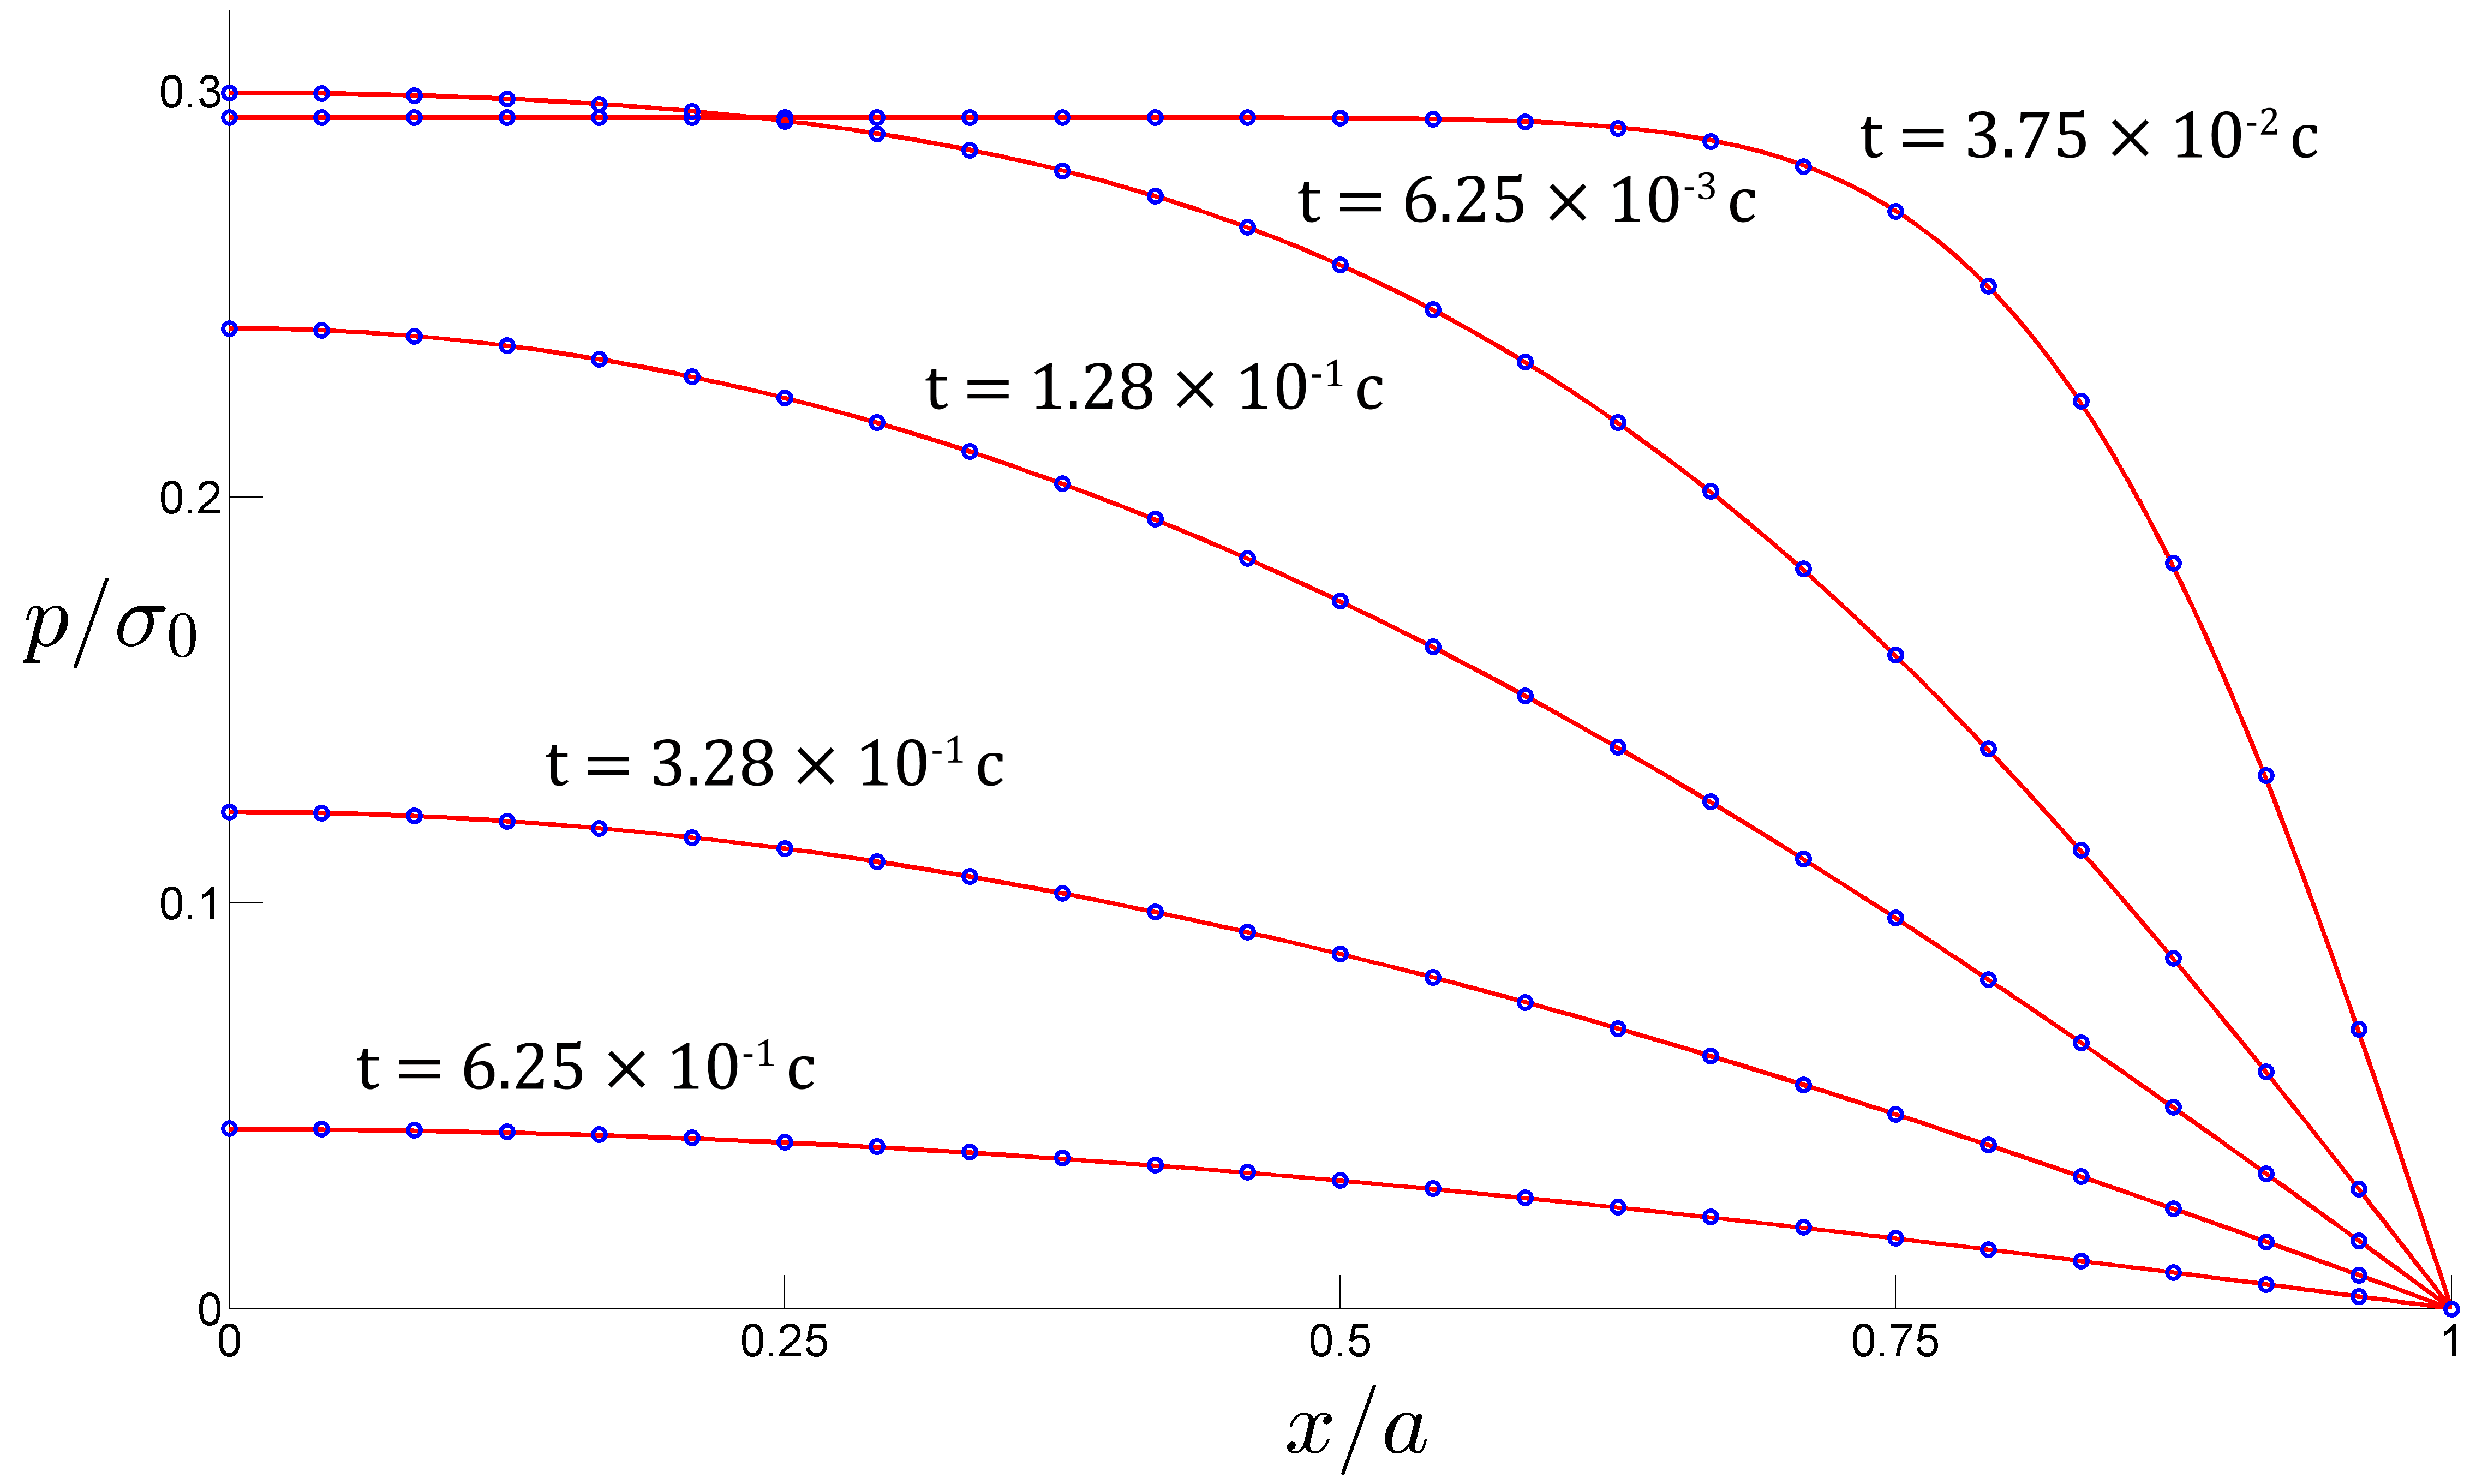
\includegraphics[width=0.95\textwidth]{./figs/pp0M.png}
\caption{Задача Манделя. Нормированное давление в различные моменты времени: красным цветом показано
аналитическое решение, синим~--- результаты расчета.}\label{fig:manp}
\end{figure}
% 
%
\begin{figure}[h!]
\centering
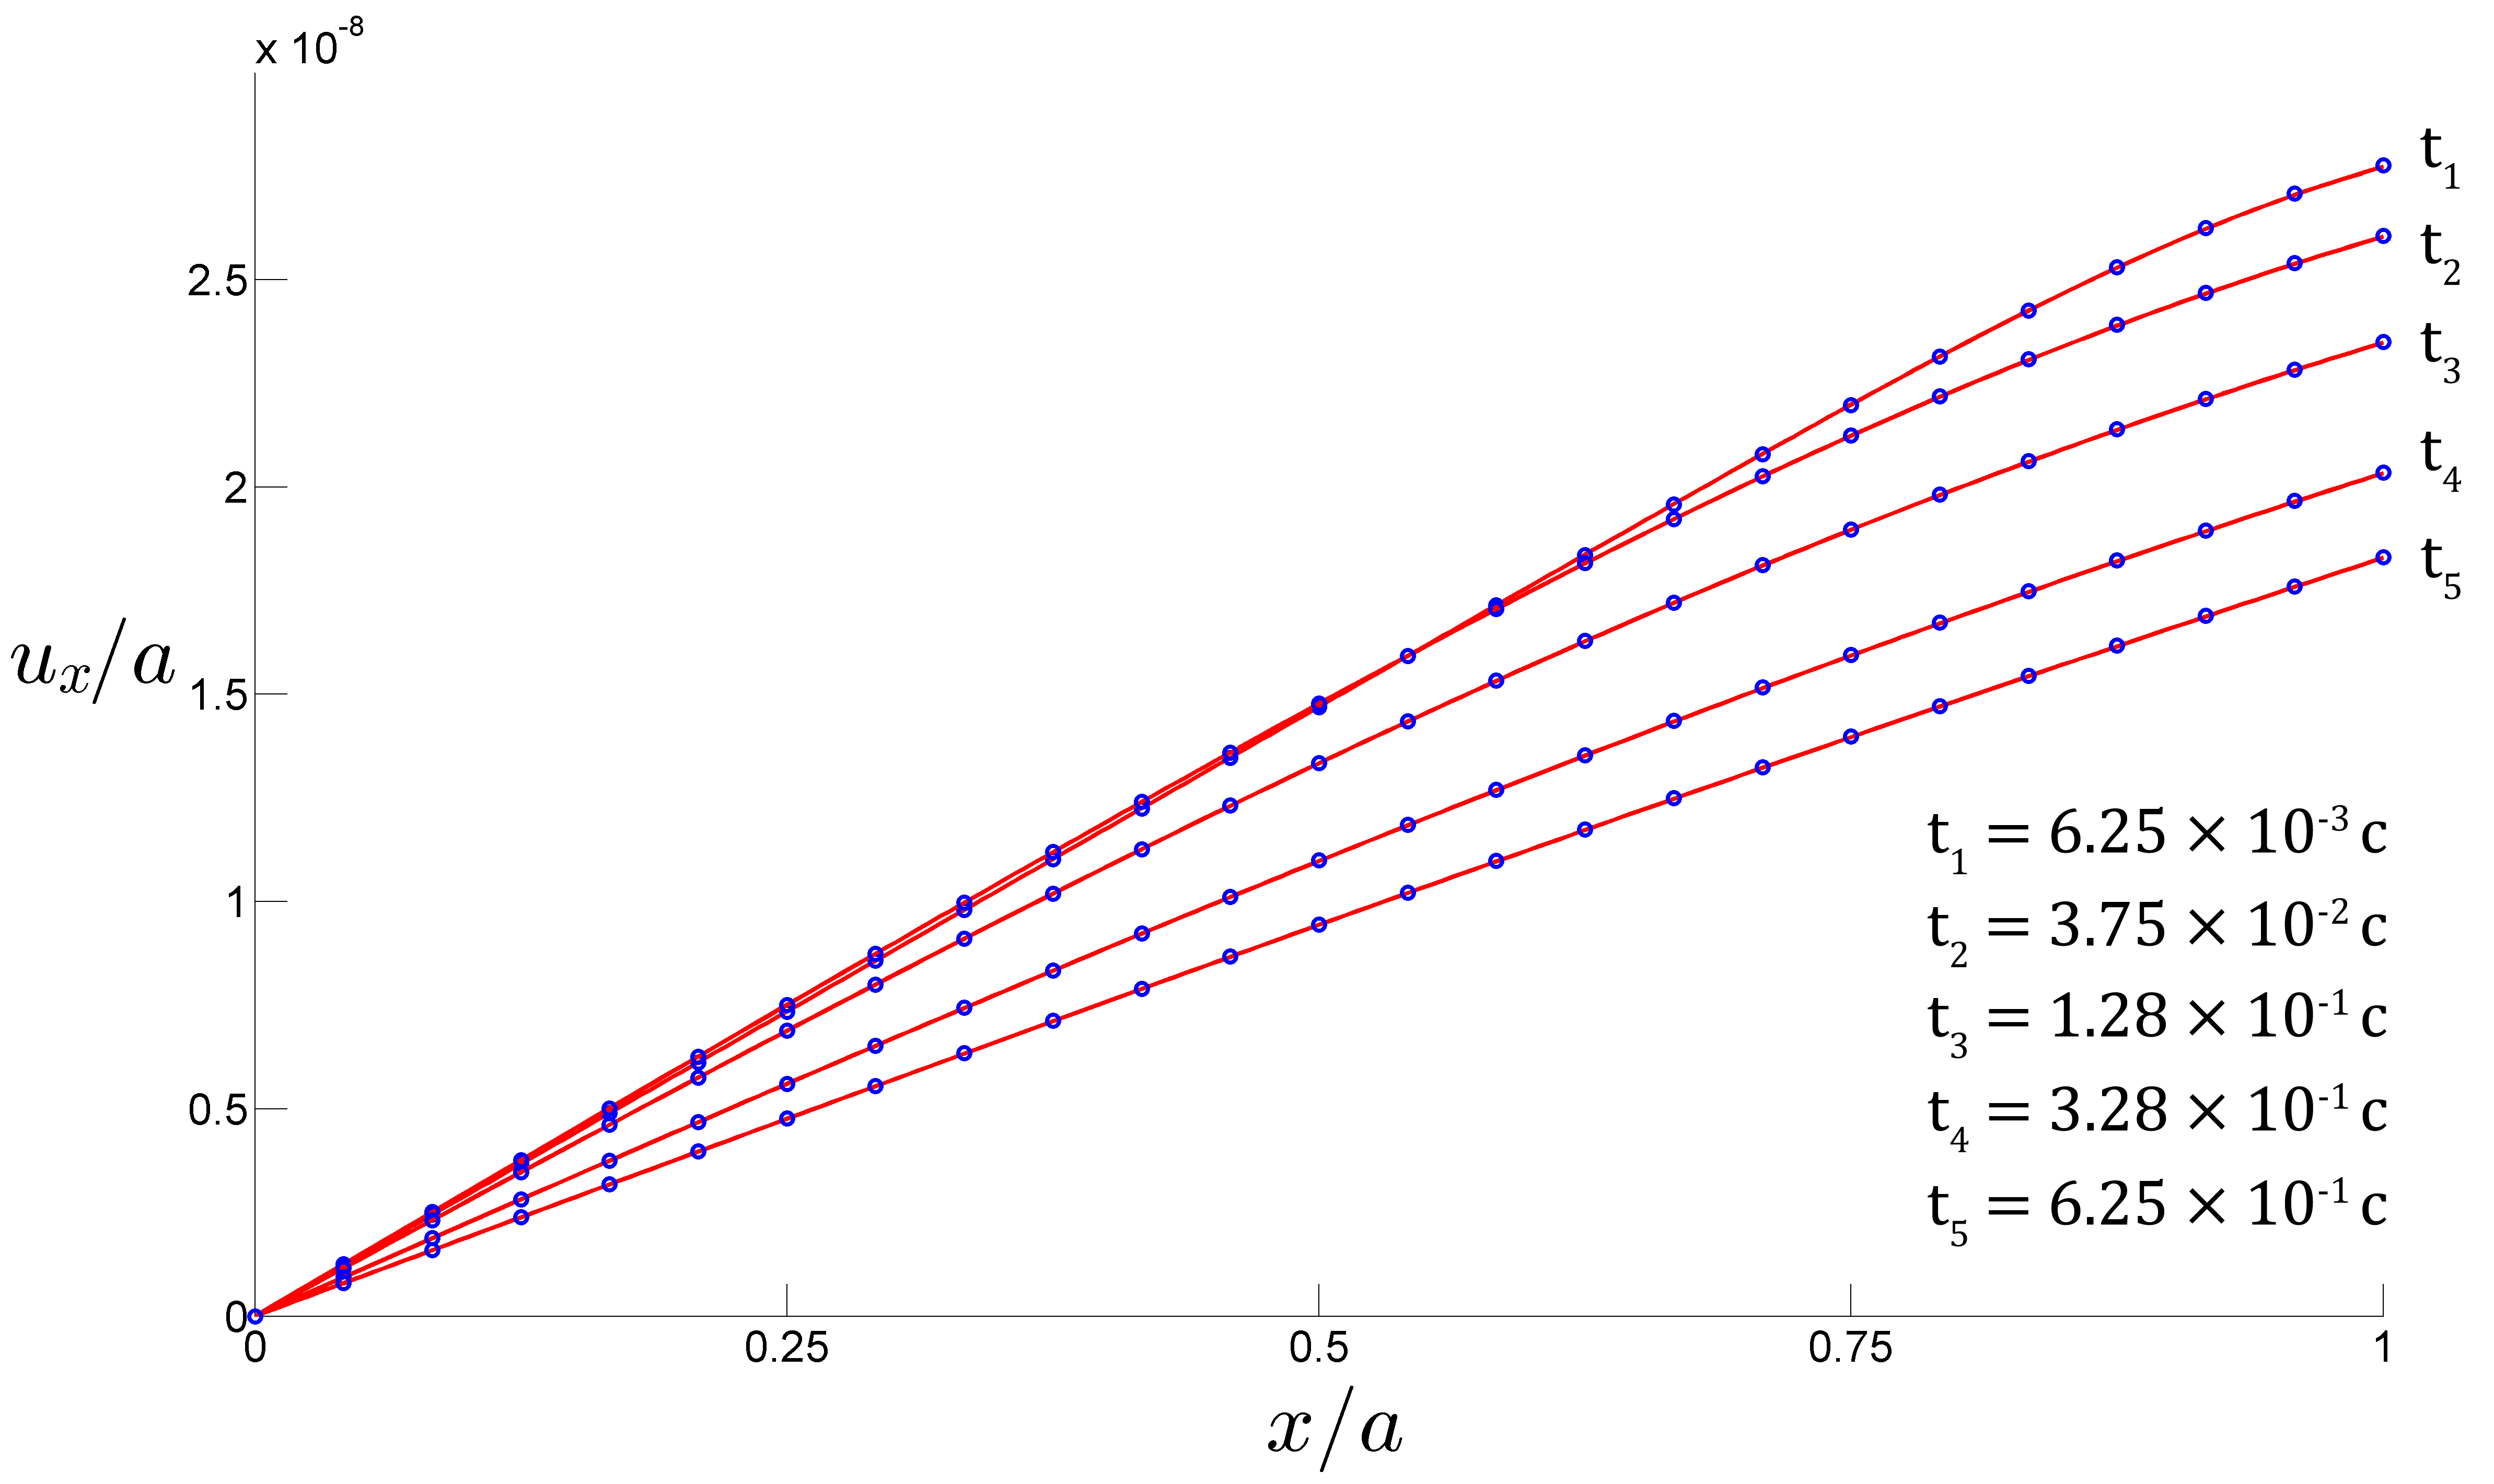
\includegraphics[width=0.85\textwidth]{./figs/uux0M.png}
\caption{ Задача Манделя. Нормированное перемещение $u_x$ в различные моменты времени: красным цветом показано
аналитическое решение, синим~--- результаты расчета.}\label{fig:manux}
\end{figure}
%
%
\begin{figure}[t!]
\centering
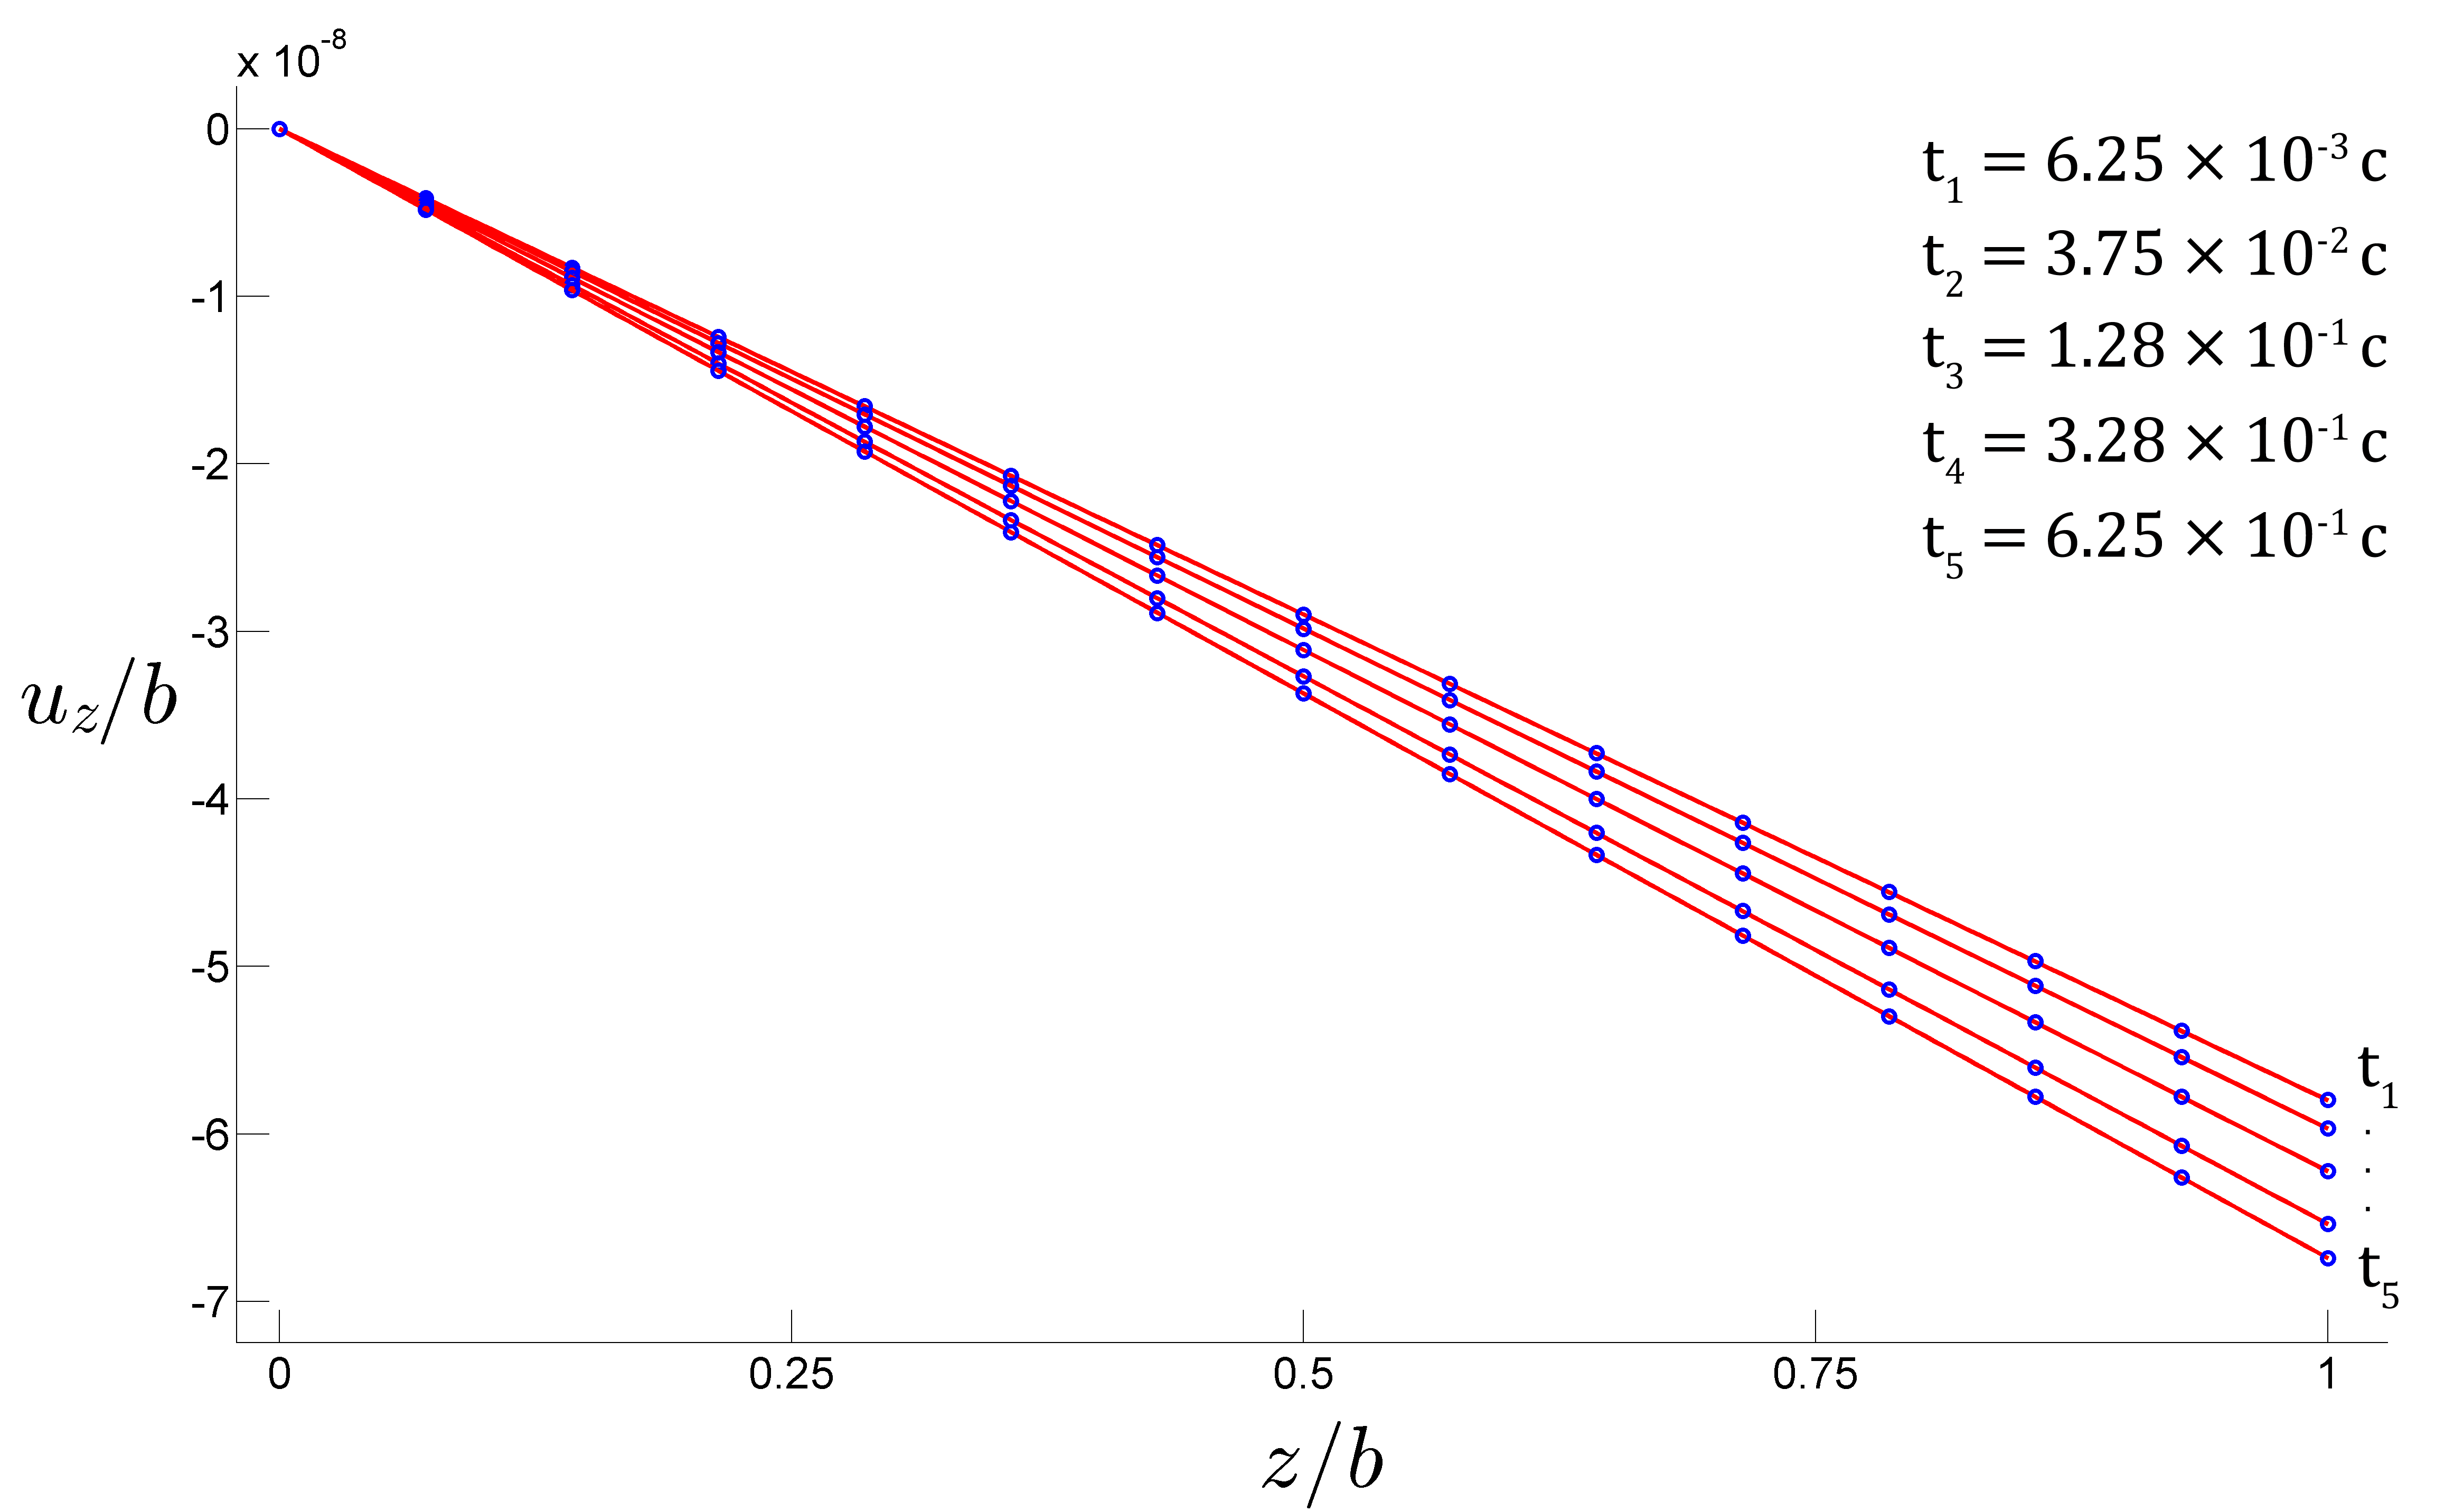
\includegraphics[width=0.85\textwidth]{./figs/uuz0M.png}
\caption{ Задача Манделя. Нормированное перемещение $u_z$ в различные моменты времени: красным цветом показано
аналитическое решение, синим~--- результаты расчета.}\label{fig:manuz}
\end{figure}
%

%
\begin{figure}[h!]
\centering
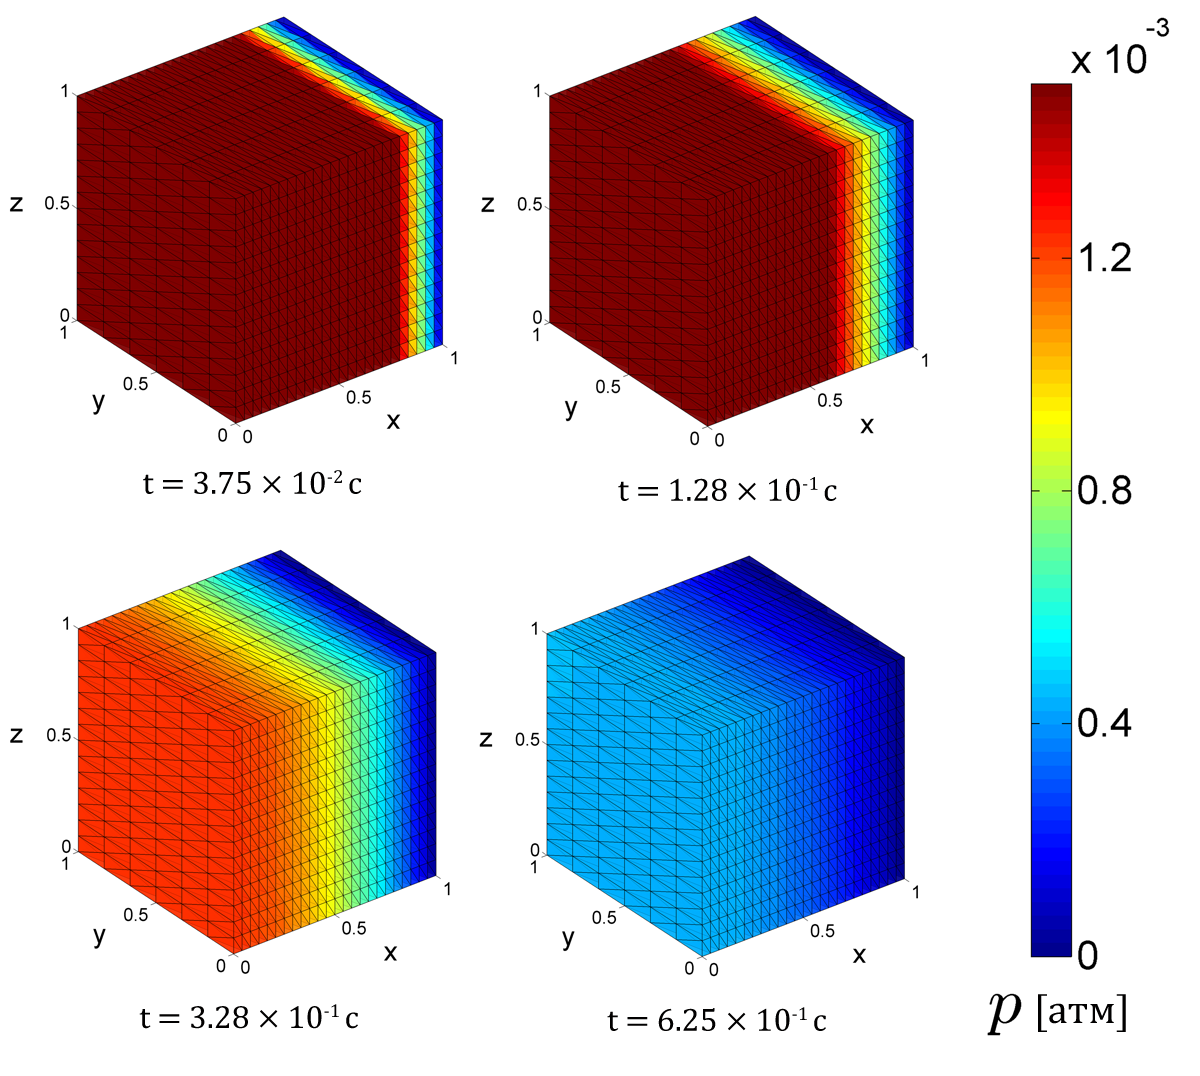
\includegraphics[width=0.73\textwidth]{./figs/prM.png}
\caption{ Задача Манделя. Распределение давления в последовательные моменты времени.}\label{fig:manpp}
\end{figure}
%

\subsection{Пороупругий пласт при наличии скважин}

Рассмотренные в предыдущих разделах постановки задач предназначены для валидации
разработанного авторами программного комплекса. Для них известно точное аналитическое решение,
но фактически данные задачи являются одномерными или двумерными.
В данном разделе рассматривается полностью трехмерная задача о перераспределении поля пластового давления
при работе двух скважин различной ориентации. К сожалению, эта задача не имеет точного аналитического решения, но иллюстрирует
возможности программного комплекса и позволяет качественно оценить достоверность полностью трехмерного моделирования задачи фильтрации в пороупругой среде в рамках разработанных алгоритмов.

Для расчетов использовалась область с линейными размерами $L_x$, $L_y$, $L_z$,
внутри которой расположены две скважины, полностью перфорирующие пласт. 
Скважины моделируются с помощью линейных источника и стока мощностью
$Q$ и $-Q$ на единицу длины. Нагнетательная скважина расположена вертикально и
проходит через точки с координатами $(L_x/3, L_y/2, 0)$ и $(L_x/3, L_y/2, L_z)$,
добывающая скважина является горизонтальной и проходит через точки
с координатами $(2L_x/3, 0, L_z/2)$ и $(2L_x/3, L_y, L_z/2)$.
Схематично постановка задачи представлена на рис.~\ref{fig:2wells}.
Конкретные значения используемых для расчетов параметров приведены в табл.~\ref{tab:2wells}.
%
\begin{figure}[h!]
\centering
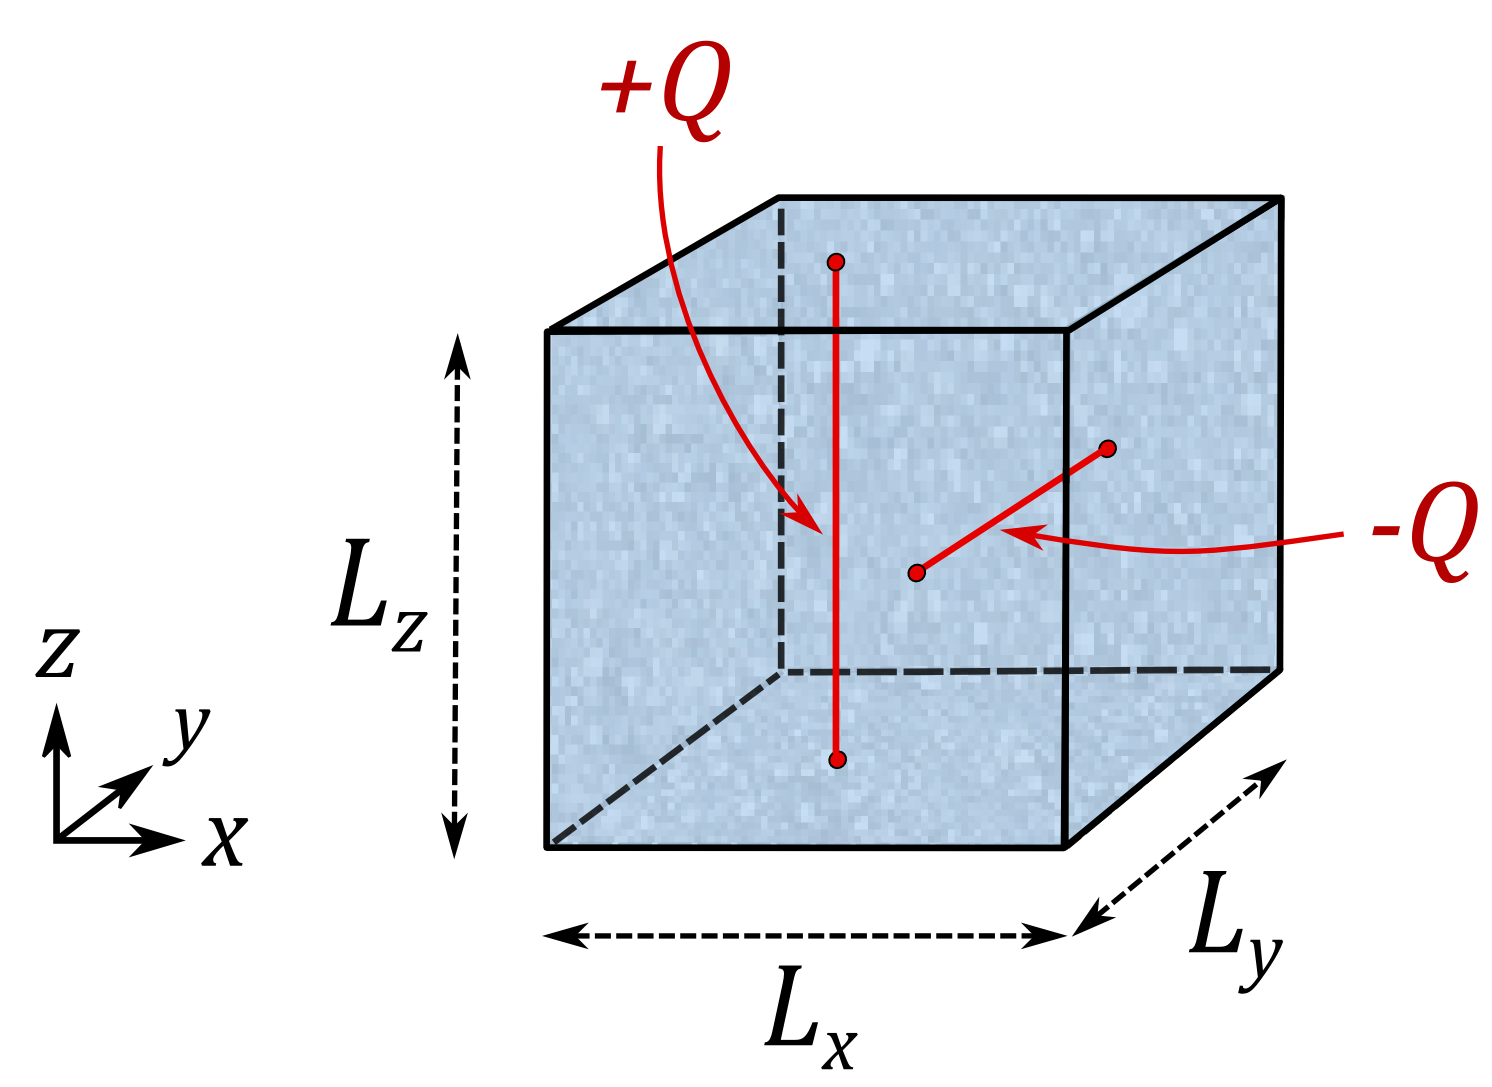
\includegraphics[width=0.65\textwidth]{./figs/2wells.png}
\caption{Схематичный вид задачи о двух скважинах.}\label{fig:2wells}
\end{figure}
% 

%%
\begin{table}[h!]
\centering
%
\renewcommand{\arraystretch}{1.5}
\renewcommand{\tabcolsep}{6 pt} 
\begin{tabular}{|c|c|c|c|c|c|c|}
\hline
$L_x$ & $L_y$ & $L_z$ & $|Q|$ & $t_{\text{start}}$ & $t_{\text{end}}$ & $\Delta t$\\
\hline
 $400.0$ м & $400.0$ м & $400.0$ м & $20.0 \text{ м}^2/\text{cутки}$ & $0.0$ ч & $20.0$ ч & $1.0$ ч\\
\hline
\end{tabular}
%
\caption{Параметры для численного расчета задачи о двух скважинах.}\label{tab:2wells}
\end{table}
%%
%

Предполагается, что пороупругая область изолирована от внешней среды.
На границе области заданы нулевые перемещения и нулевой поток, т.е. 
$\partial p/ \partial n = 0$. В качестве начального условия задавалось состояние покоя
при давлении $p = 100$ атм и нулевых перемещениях точек среды.

Для численных расчетов использовалась тетраэдральная сетка, состоящая из 
$N_{nodes} = 29791$ узлов и $N_{elems} = 162000$ прямоугольных тетраэдров со сторонами
$h_x = h_y = h_z = 13.3333$ м. 

%
\begin{figure}[t!]
\centering
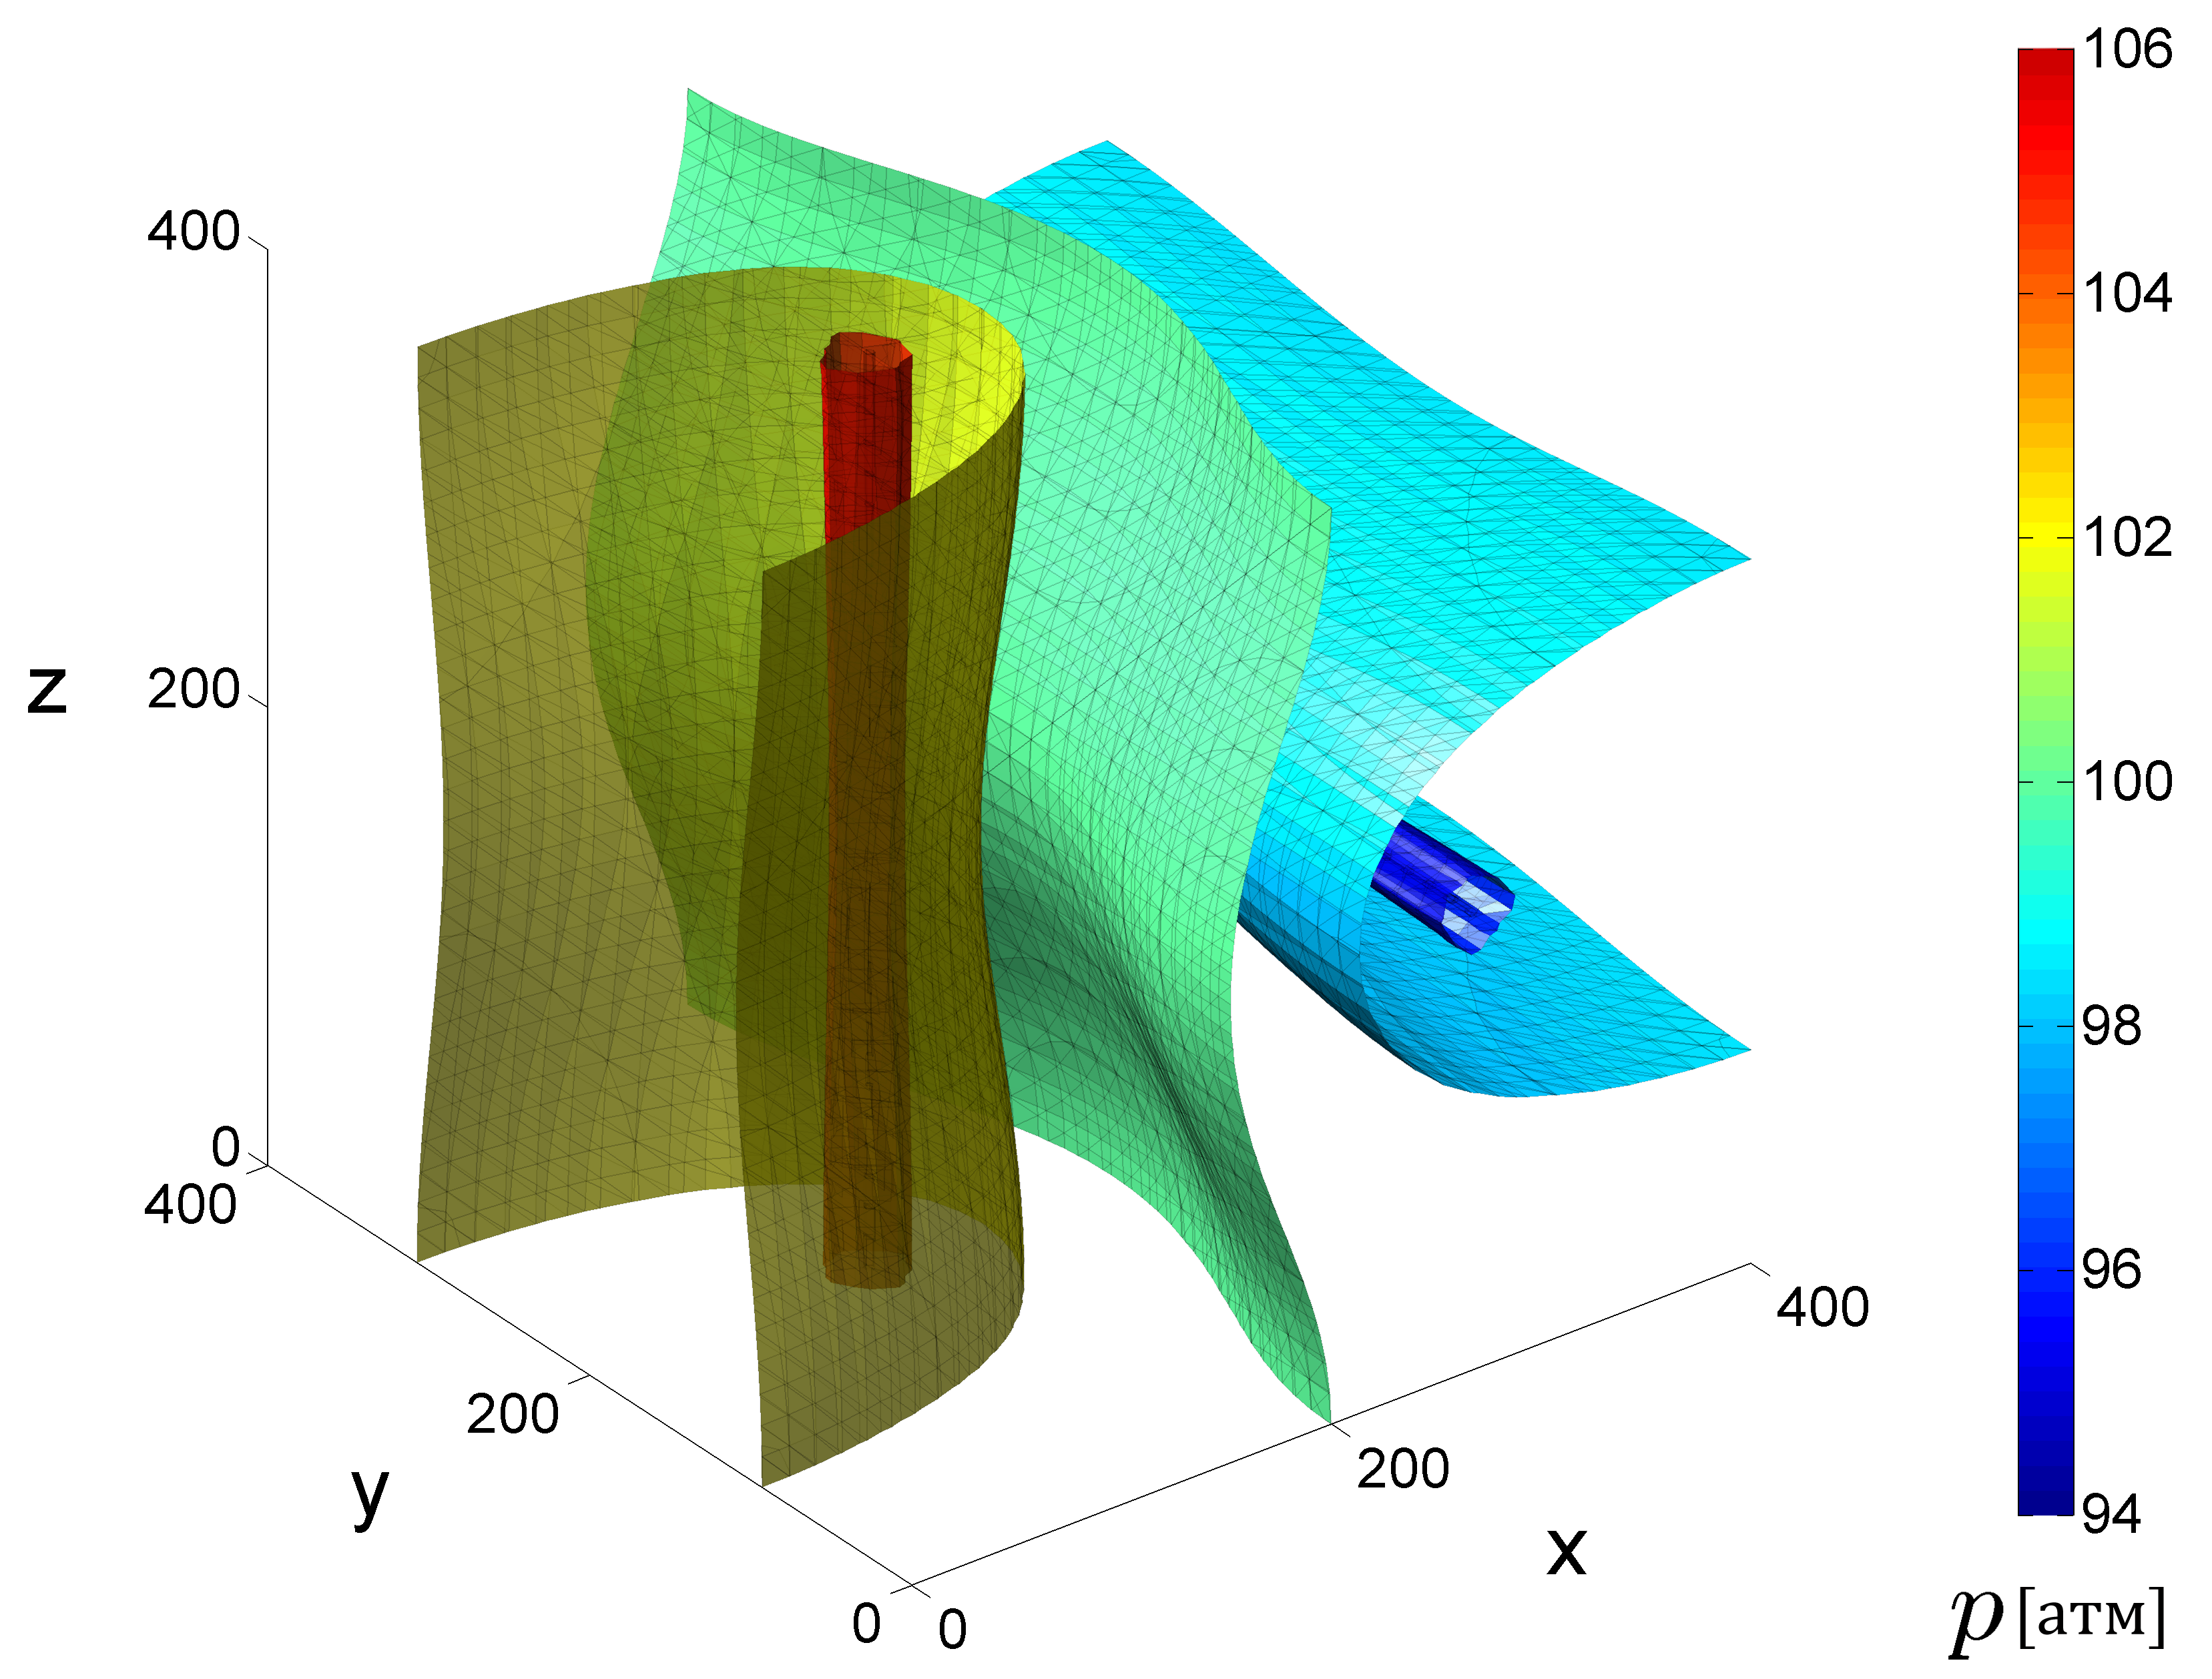
\includegraphics[width=0.8\textwidth]{./figs/iso_p.png}\\
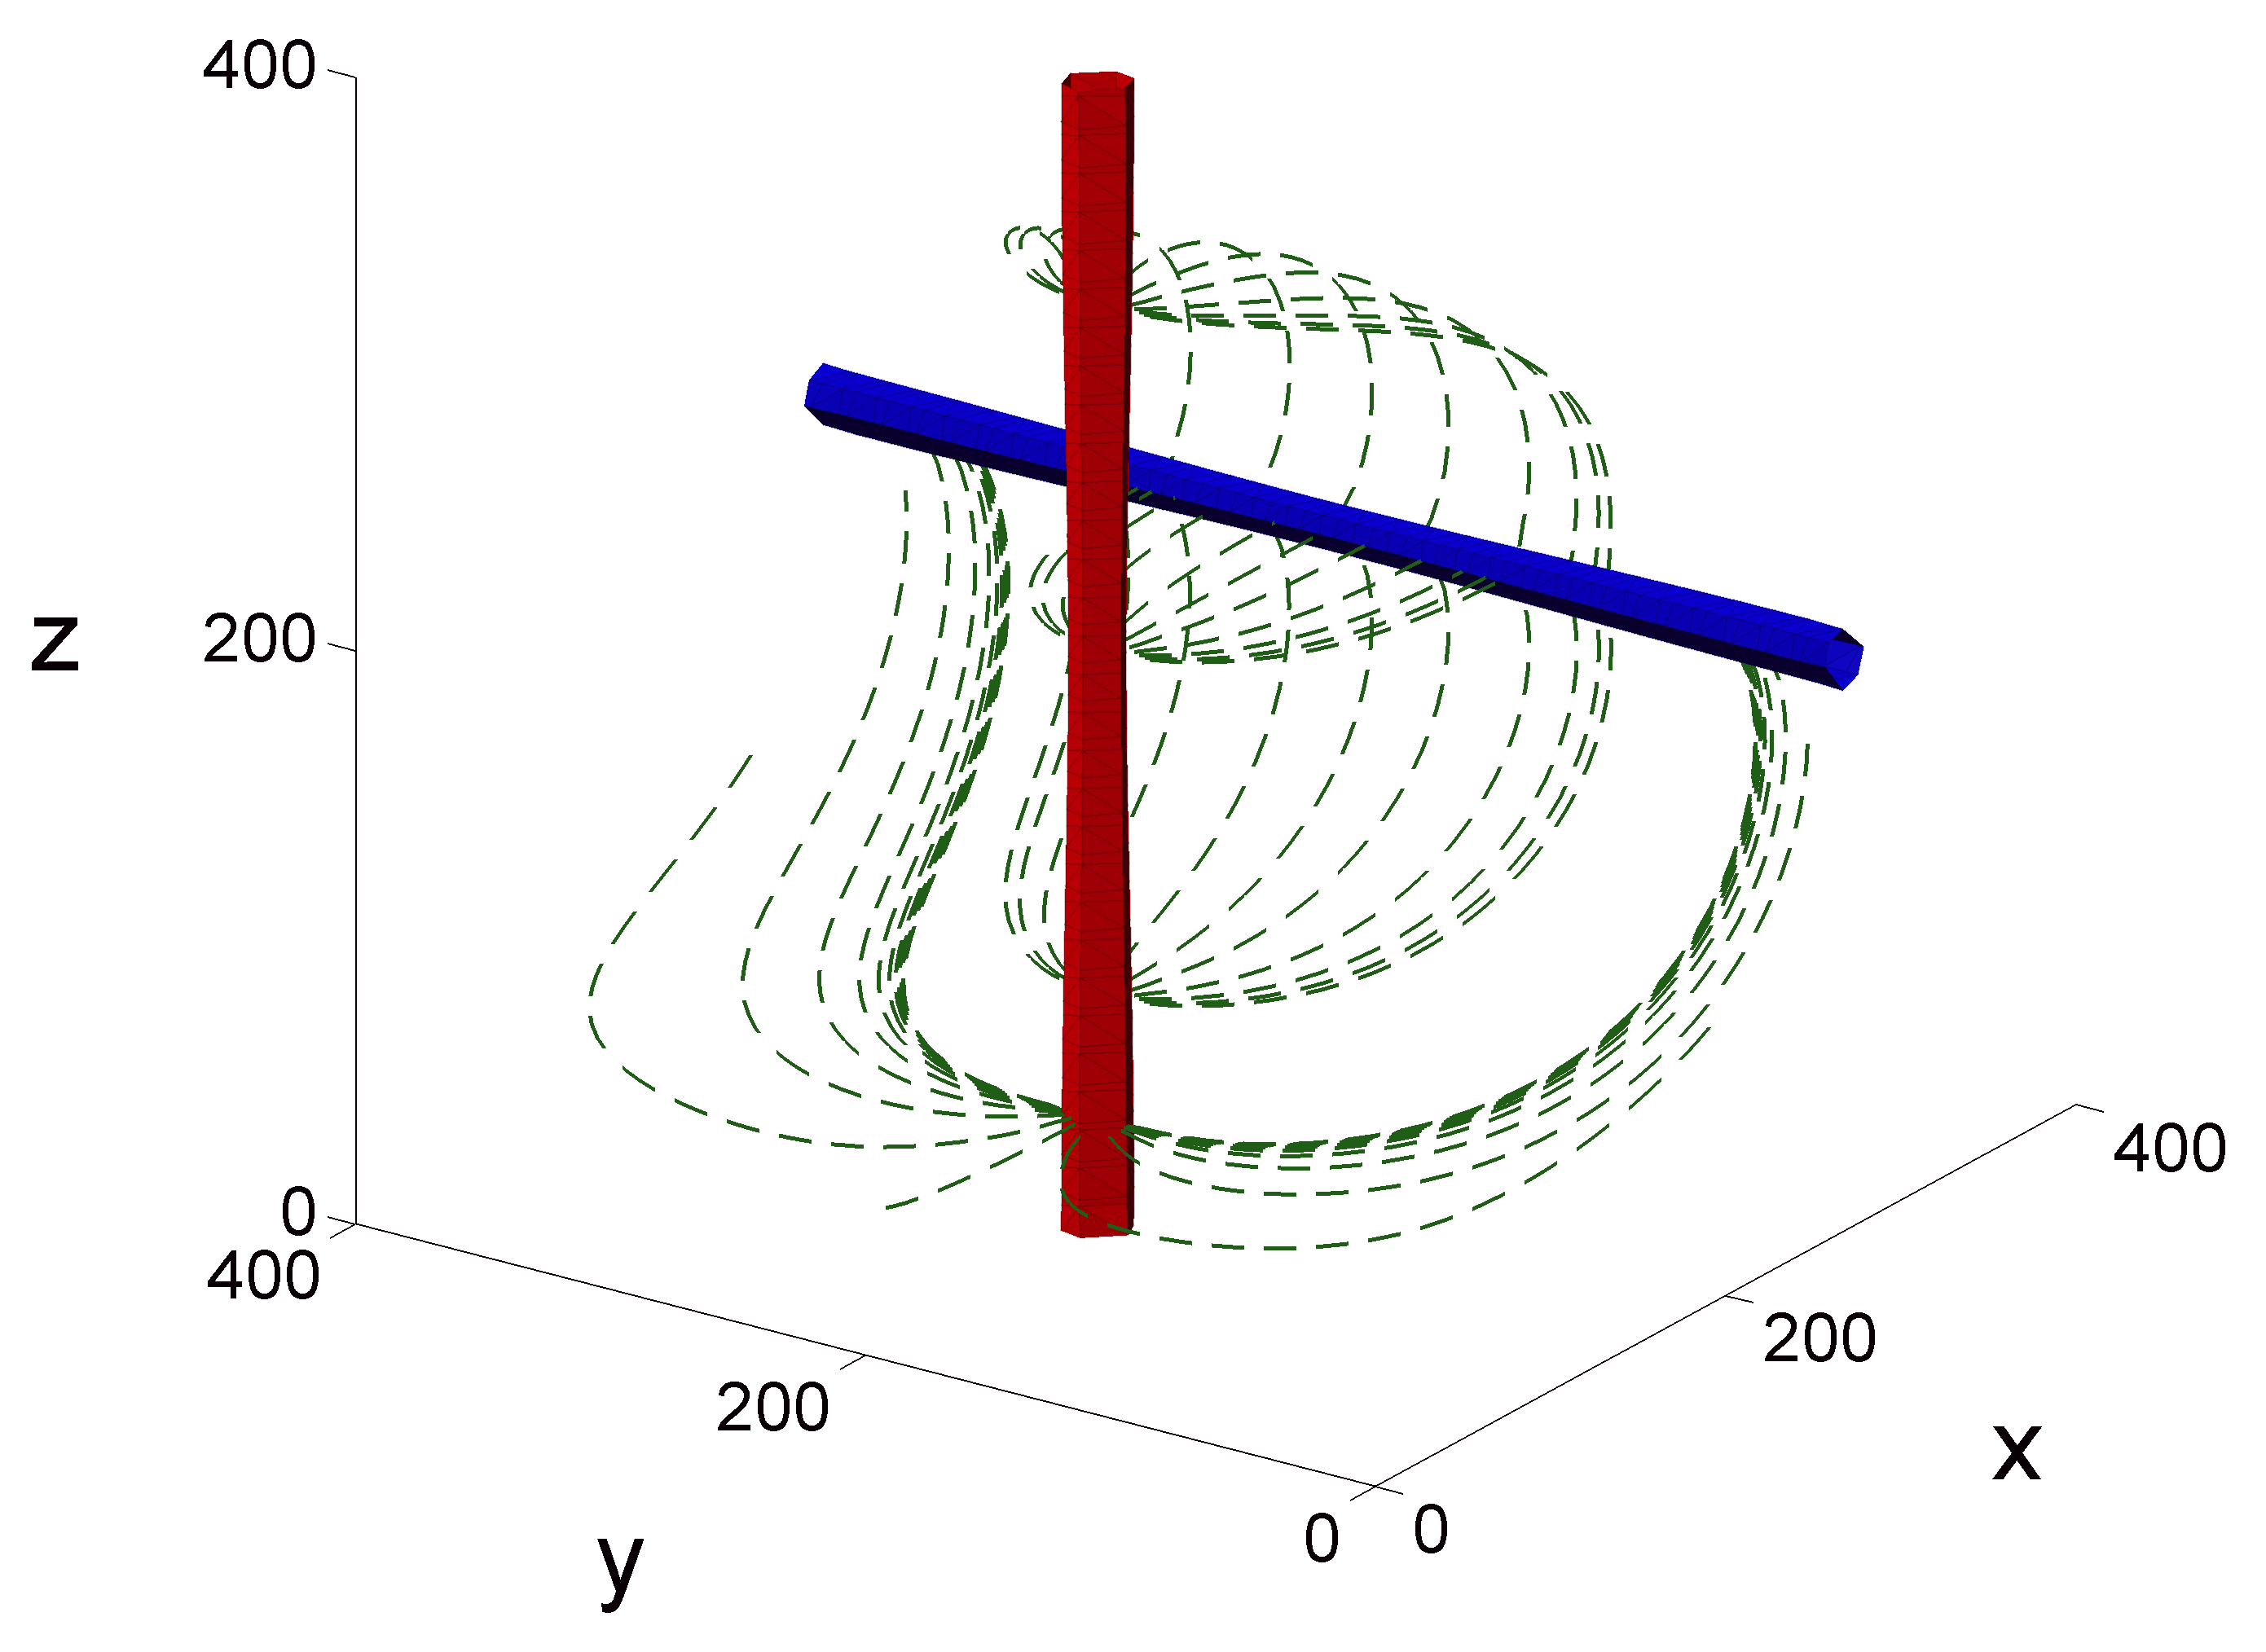
\includegraphics[width=0.8\textwidth]{./figs/str.png}
\caption{Задача о двух скважинах. Изоповерхности давления (вверху) и линии тока (внизу) в конце расчета.}\label{fig:iso}
\end{figure}
% %
% \begin{figure}[h!]
% \centering
% 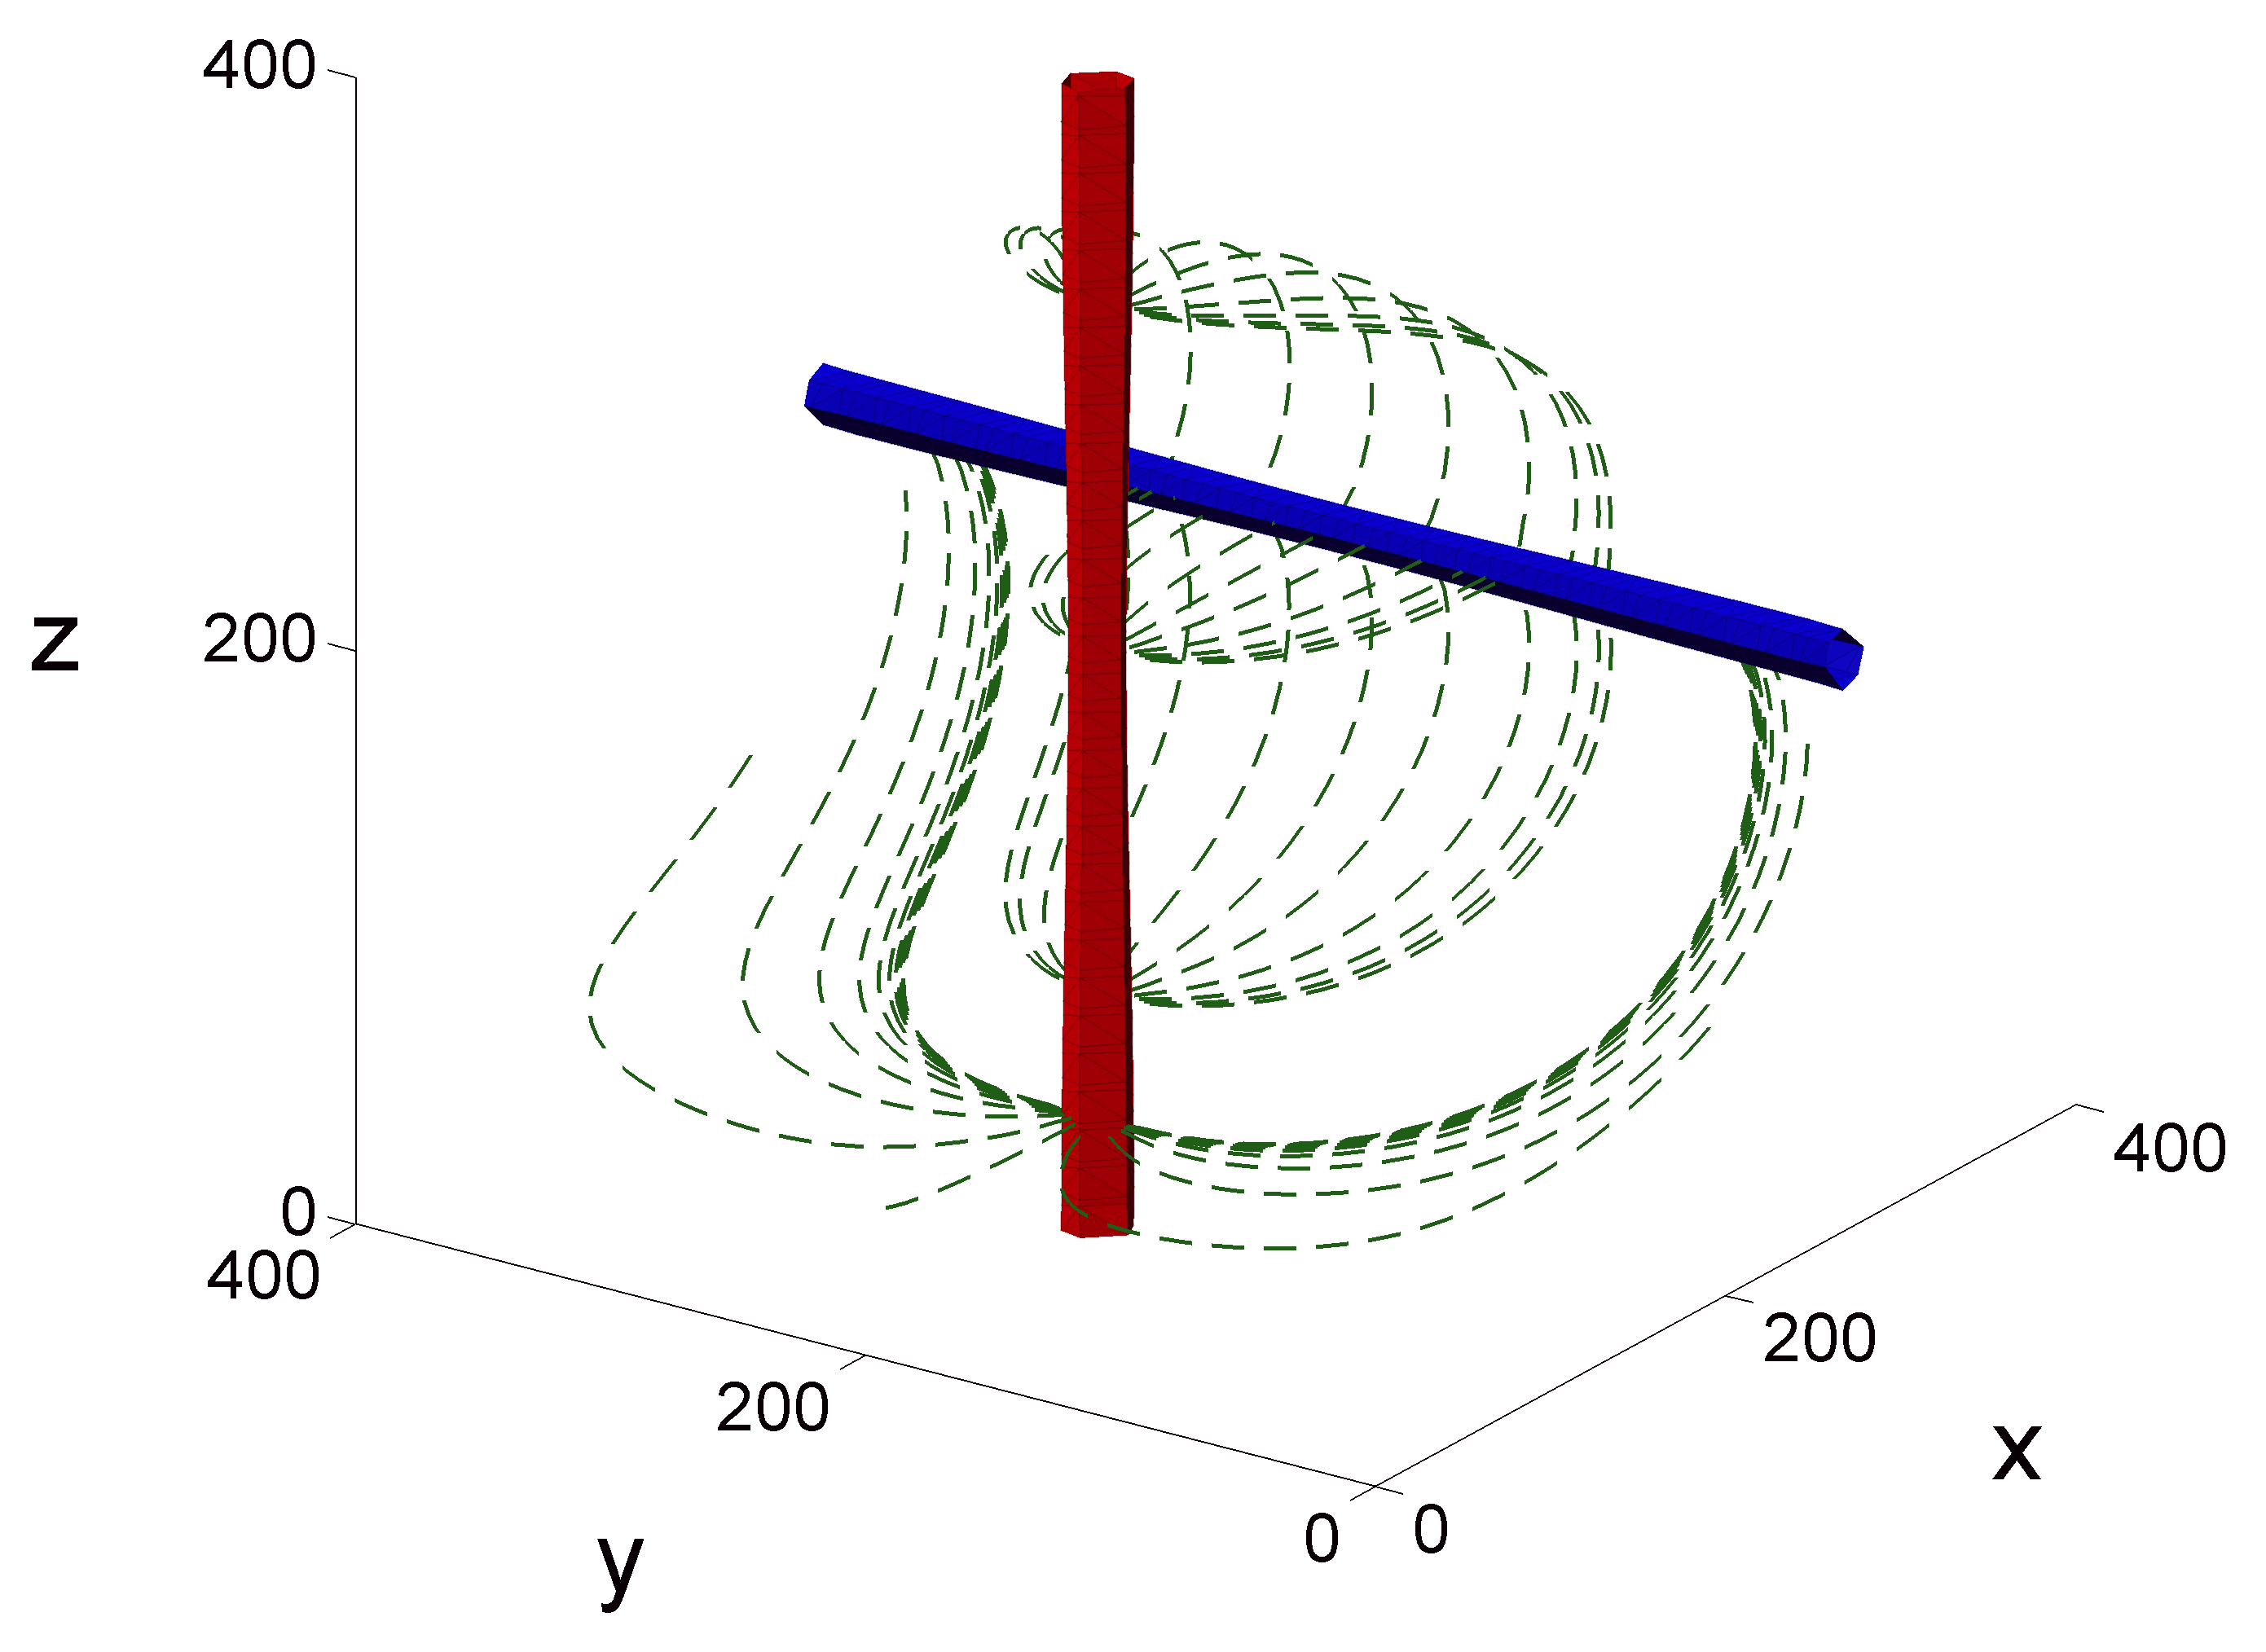
\includegraphics[width=0.83\textwidth]{./figs/str.png}
% \caption{Линии тока в конце расчета}\label{fig:str}
% \end{figure}
% 

На рис.~\ref{fig:iso} представлены несколько поверхностей уровня
порового давления (вверху) и линий тока (внизу) 
в конце моделирования при установлении псевдостационарного режима течения.
Видно, что структура течения существенно трехмерна и симметрична в силу симметричности постановки задачи.

%%%%%%%%%%%%%%%%%%%%%%%%
\settocdepth{section}

%%%%%%
\endinput
% EOF
